\documentclass[10pt]{report}
\usepackage[utf8]{inputenc}
\usepackage{graphics}
\usepackage{epsfig}
\usepackage{amssymb}
\usepackage{amsmath}
%\usepackage{ngerman}
\usepackage{latexsym}
\usepackage{float}
\newcommand{\DS}{\displaystyle}
\addtolength{\textheight}{4cm}
\addtolength{\headheight}{-2cm}


\begin{document}
\tableofcontents

\pagebreak
\section{Introduction}
        
 Der ParliamentBrowser ist eine Anwendung, welche diverse Informationen aus den Protokollen des deutschen Bundestags in komprimierter Form zusammen-führt. Neben diesen Protokollen, als Quellen der zu extrahierenden Daten, sind ihre Untergliederung in Tagesordnungspunkten, Reden, Kommentaren, Metadaten der Abgeordneten und Annotationen des Natural Language Processing, NLP, die Basis für weitere Informationsgewinnung und Darstellung gewünschter Erkenntnisse. Die so gewonnenen Daten werden kumuliert, komprimiert und visualisiert, um eine detaillierte Aufbereitung von Analysen zu ermöglichen. Dazu werden die Bundestagsprotokolle der 19. und 20. Legislaturperiode per scraping heruntergeladen, in geeignete Datenstrukturen gespeichert und in eine MongoDB übertragen. \\\\
 Auf der Frontpage sind erste Informationen zu der Anzahl zusammengetragener Reden und Kommentare zu finden. Ferner sind die häufigsten Redner dieser analysierten Reden namentlich genannt.  \\\\
 Im Folgenden werden schrittweise die Eigenschaften (Features) der Applikation aufgeführt und beschrieben. Wir beginnen zunächst von rechts nach links entlang der oberen Navigationsleiste und erläutern die dahinter liegenden Funktionen.      
 \\\\\\\\    
\begin{figure}[H]
	\begin{center}		
		\scalebox{0.35}{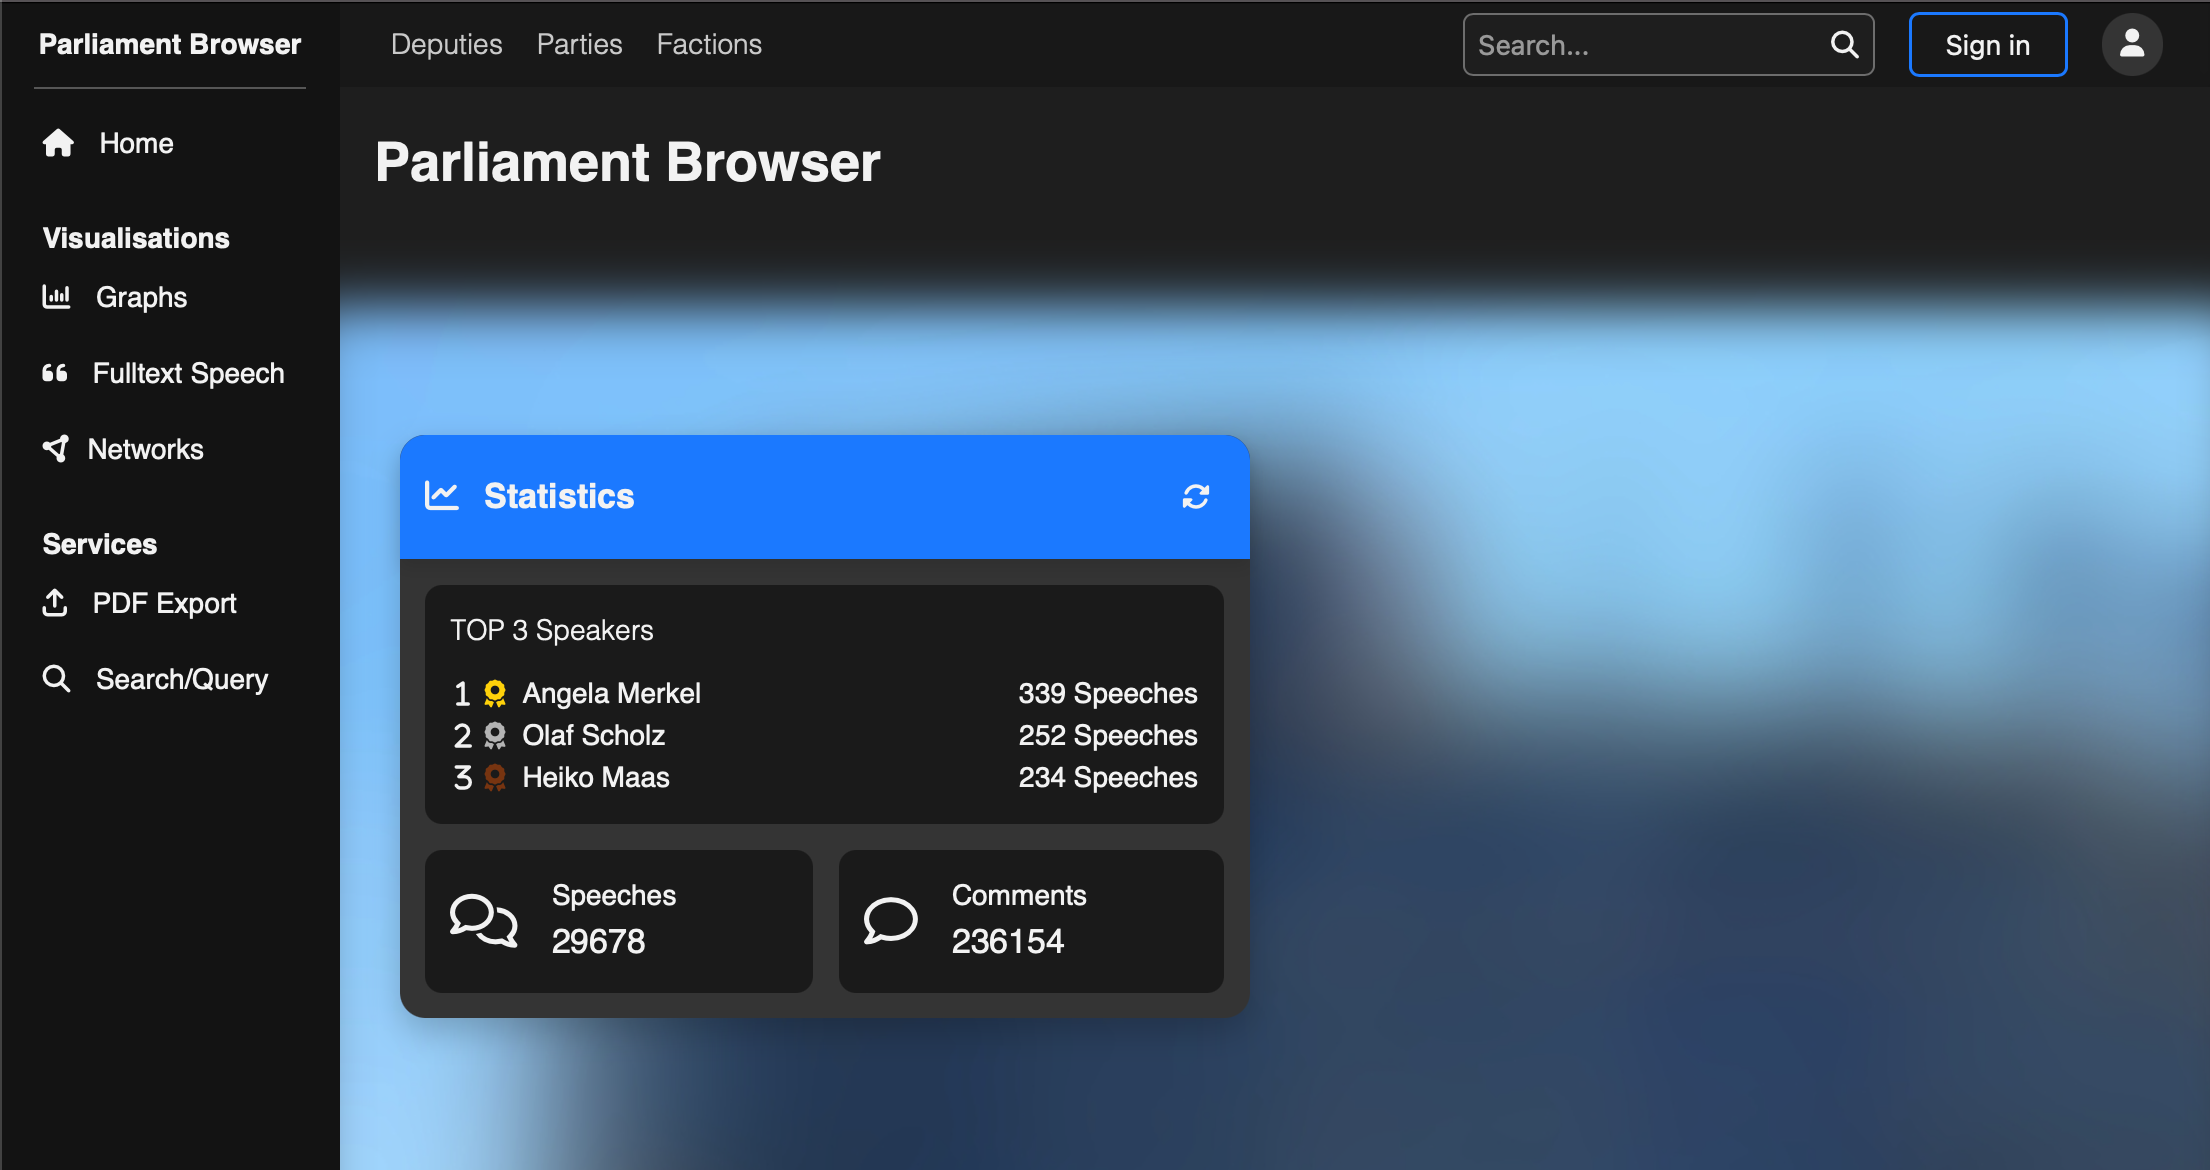
\includegraphics{home_page1}}
  	 \end{center}
	\caption{Parliament Browser $\rightarrow$  Route:  /}	
 \end{figure} 

\chapter{Features: Home und obere Navigationsleiste }
\section{Home $\quad\rightarrow\quad$  Route:  /}
In Abbildung 1. sind alle relevanten Textfelder mit den dahinter liegenden Features der Applikation zu sehen. Diese sollen im Folgenden veranschaulicht und erläutert werden. 
Beginnen wir oben rechts mit Home /:  \\...  der Parliament Browser. \\
\section{SignIn $\quad\rightarrow\quad$  Route:  /login}
Über ein mit dem Sign In Button erreichbare Anmeldewebsite können sich Nutzer im Parliament Browser anmelden, wodurch weitere Funktionalitäten zur Verfügung gestellt werden. Auf dieser Anmelde-Seite erwartet die Benutzer\_in ein Formular die Login-Daten.   \\\\

    
\begin{figure}[H]
	\begin{center}		
		\scalebox{0.3}{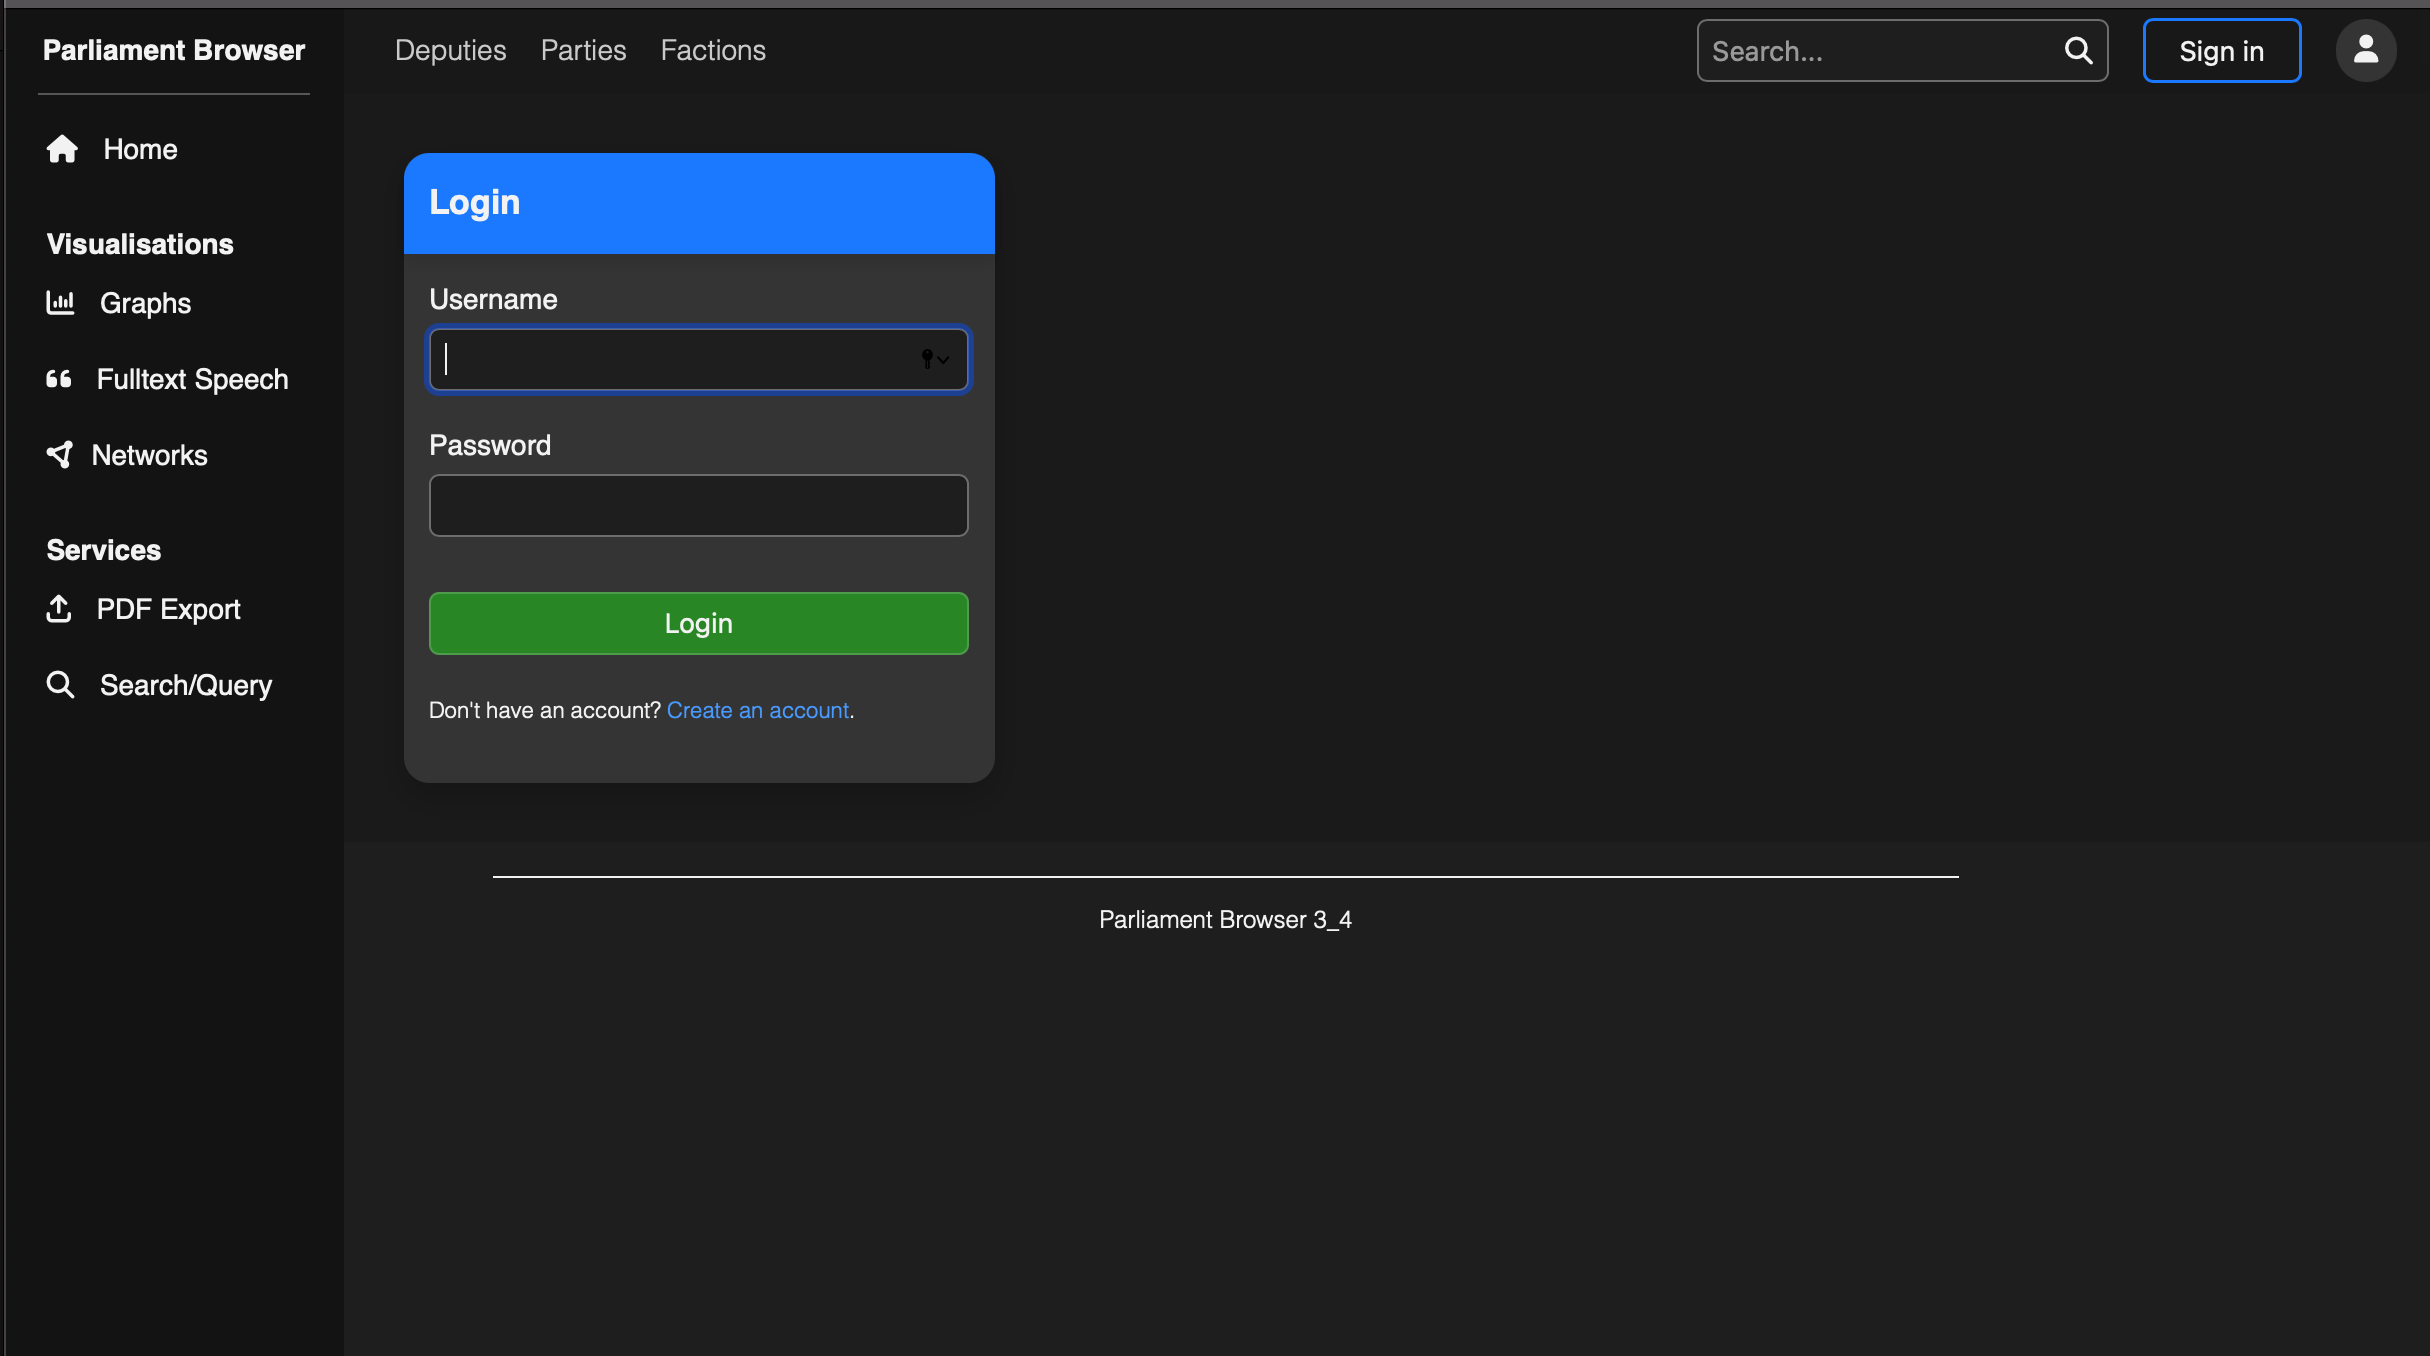
\includegraphics{signIn_page1}}
  	 \end{center}
	\caption{Login $\rightarrow$  Route:  /login }
\end{figure}


\noindent Die Eingabe von Username und Password sind erforderlich, um weitere Rechte in Anspruch zu nehmen. Falls noch kein Account vorhanden ist, besteht die Möglichkeit einen solchen Account zu eröffnen, indem man auf 'Create an account' klickt.
	
\section{Create-Account $\quad\rightarrow\quad$  Route:  /create-account}  	
	
\noindent  Zur Registrierung sind, abgesehen von Username und einem zu wählenden Passwortes, noch weitere Daten erforderlich. E-Mail Adresse und Geburtsdatum dienen der genaueren Identifikation des Nutzers.\\\\
\begin{figure}[H]
	\begin{center}		
		\scalebox{0.3}{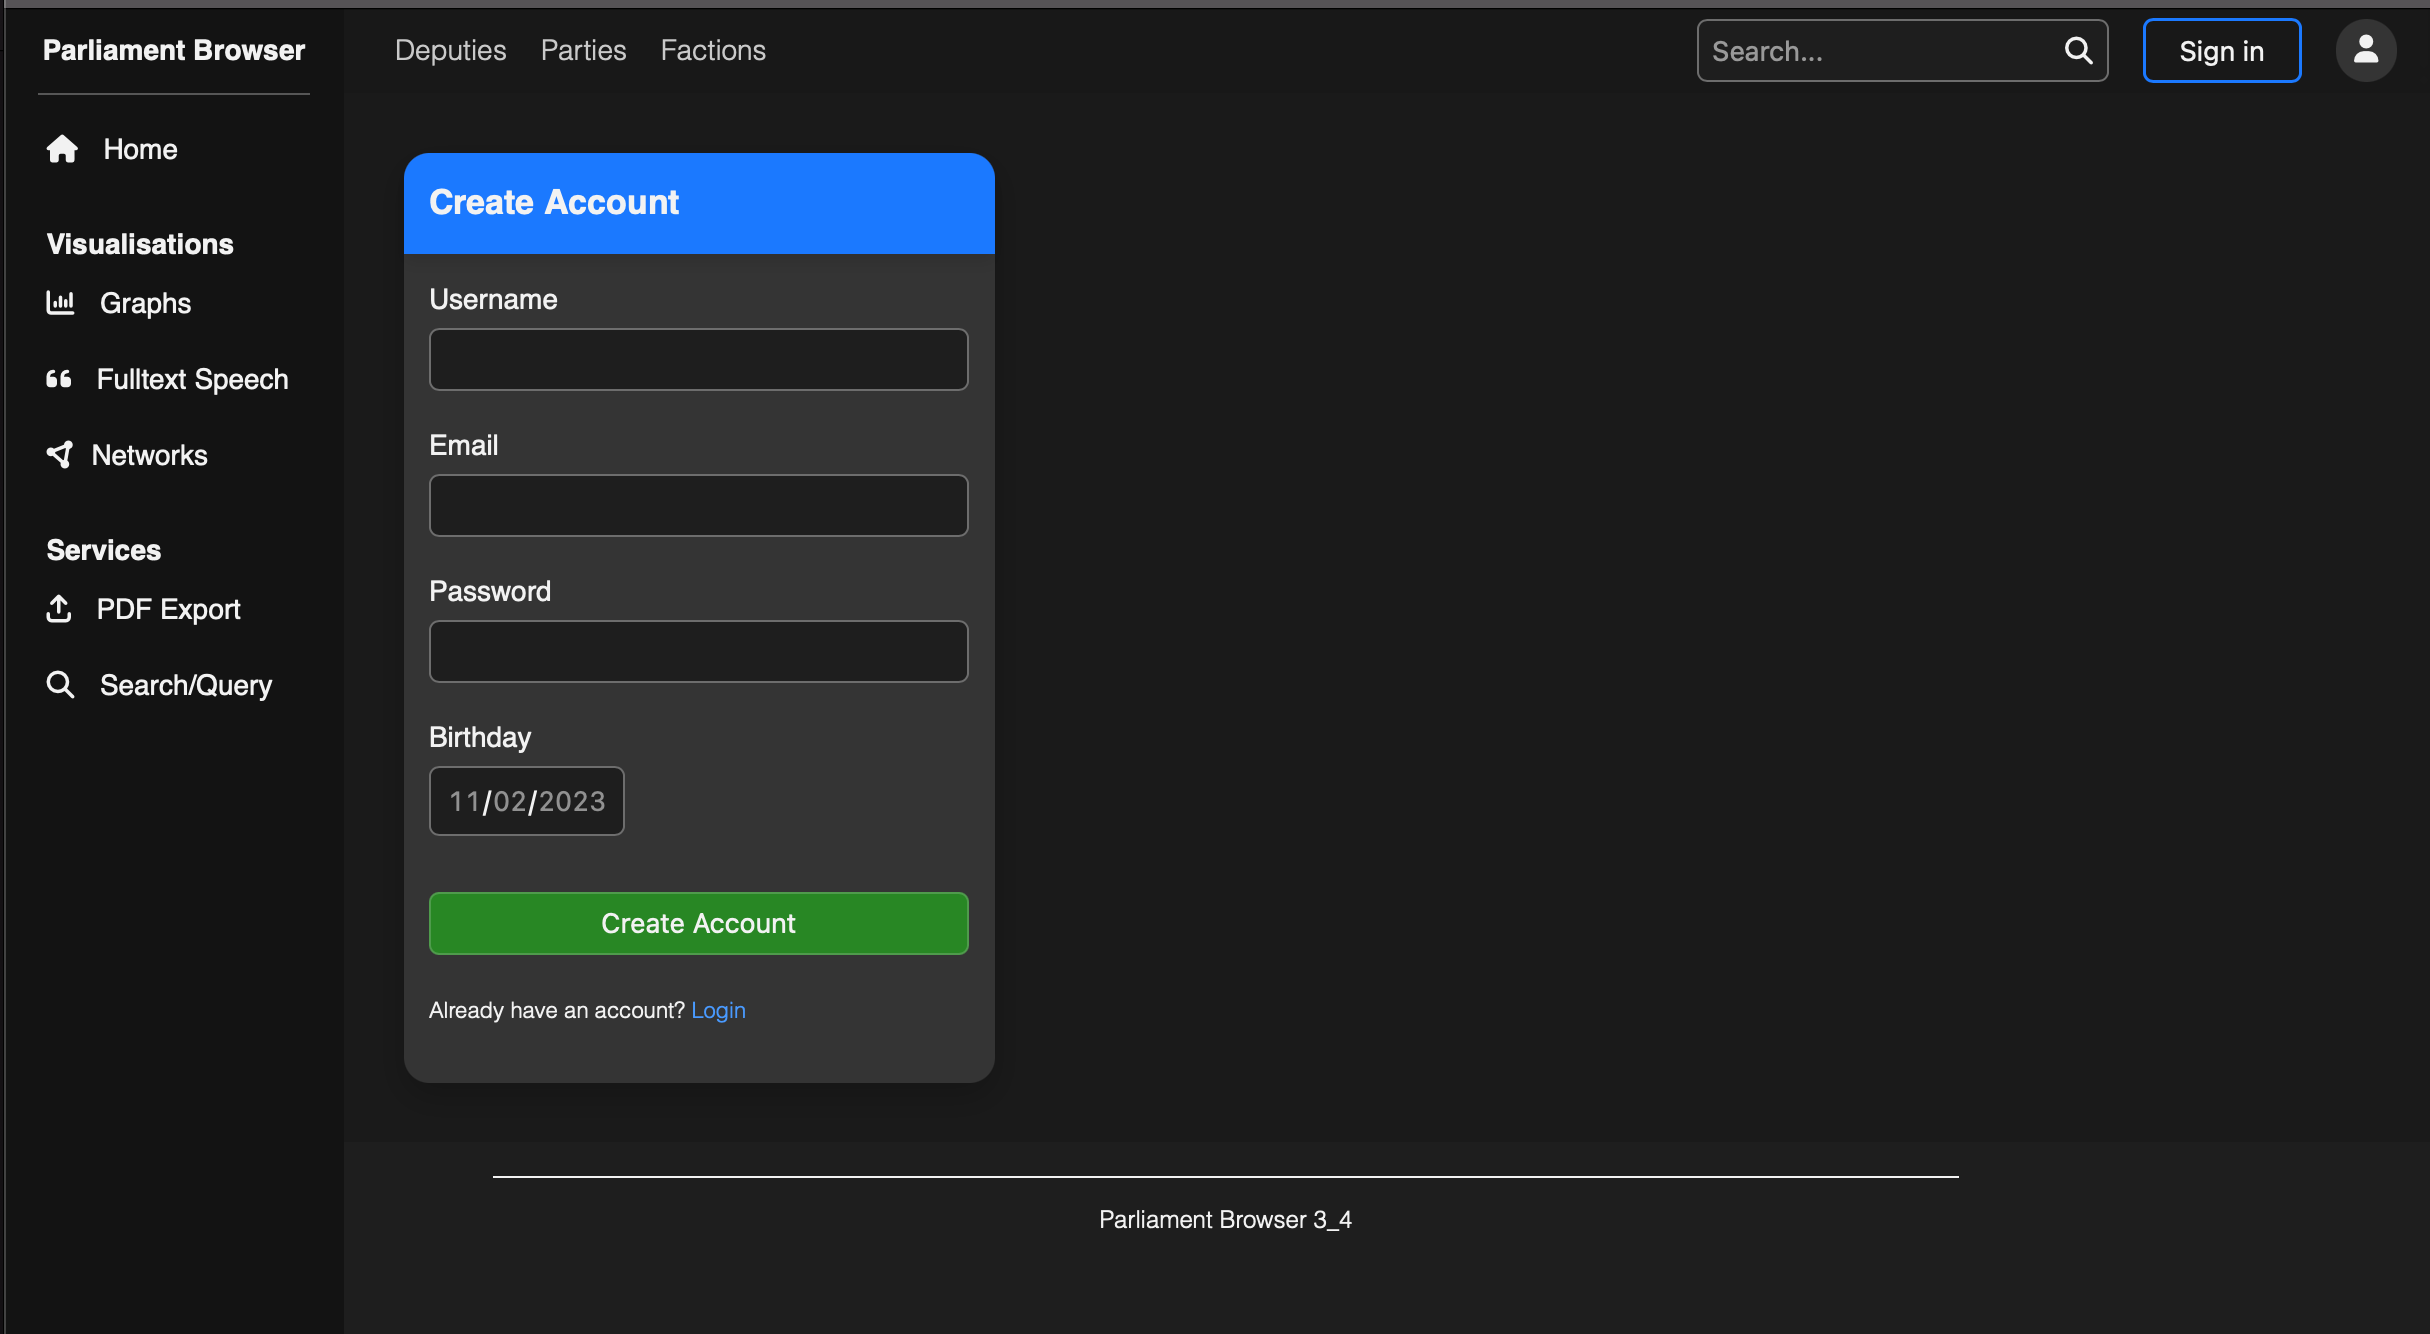
\includegraphics{signIn_page2}}
  	 \end{center}
	\caption{Create Account $\quad\rightarrow\quad$  Route:  /create-account}	
 \end{figure}



\section{Profile $\quad\rightarrow\quad$  Route:  /profile}
Im Menü 'Profile', erreichbar über das User Icon rechts in der oberen Menüleiste, besteht die Möglichkeit, persönliche Daten (Credentials) wie Passwort, Email, Username und Geburtsdatum zu bearbeiten. \\\\

\section{Admin Dashboard $\quad\rightarrow\quad$  Route:  /admin-dashboard}
Mit der Admin-Rolle stehen mehrere weitere Funktionalitäten zur Verfügung.  \\\\
Zum AdminDashboard, ebenfalls erreichbar über das User Icon rechts in der oberen Menüleiste, haben nur Administratoren Zugriff. Der Zugriff erfordert deshalb zwingend eine vorherige Anmeldung. Im Dashboard können dann User angelegt und gelöscht (delete), Features angelegt und Rechte authorisiert werden, sowie diese eingeräumten Rechte wieder weggenommen oder ent-authorisiert werden. \\
Ein weiteres Feature, welches nur Admins vorbehalten ist, 
besteht im nochmaligen Aufrufen/Laden von XML Dateien zum wiederholten Parsen.\\\\

\section{General Search $\quad\rightarrow\quad$  Route:  /searchGeneral}
Die Allgemeine Suche stellt einen schnellen Weg dar, den Parliament Browser nach beliebigen Suchbegriffen zu durchsuchen. 
Nach Bestätigung der Suche mit Enter oder dem Klicken auf die Lupe, werden simultan Redner, Kommentare und Reden nach dem gesuchten Begriff durchsucht und die Ergebnisse anschließend auf entsprechenden Panels angezeigt.
Zur Suchbeschleunigung wird unter anderem die Volltext-Suche in der MongoDB verwendet.\\\\

\noindent Wechseln wir nun zum linken Ende der oberen Navigationsleiste:
\newpage

\section{Deputies $\quad\rightarrow\quad$  Route:  /deputies}
Diese Routen führen uns zu Informationen über die Parlamentarier:innen, seien es Abgeordnete aus früheren Legislaturperioden oder dem aktuellen Bundestag. In der Liste sind Redner:innen zu finden, mit Listen aller  ihrer Beiträge, oder schlicht Sitzungsteilnehmer:innen, die nicht regelmässig an Debatten teilnehmen. Falls vorhanden, wird ein Bild des/der Abgeordneten angezeigt.\\\\
Die Liste ist auf eine Größe von 100 Rednern pro Seite begrenzt. Mit den 'Back/Next' Buttons können die etwa 40 Seiten durchgeblättert werden.
Fraktions- und Parteizugehörigkeit, die nicht immer übereinstimmen, runden den Inhalt der ersten Seite der Deputies ab. \\\\


\begin{figure}[H]
	\begin{center}		
		\scalebox{0.28}{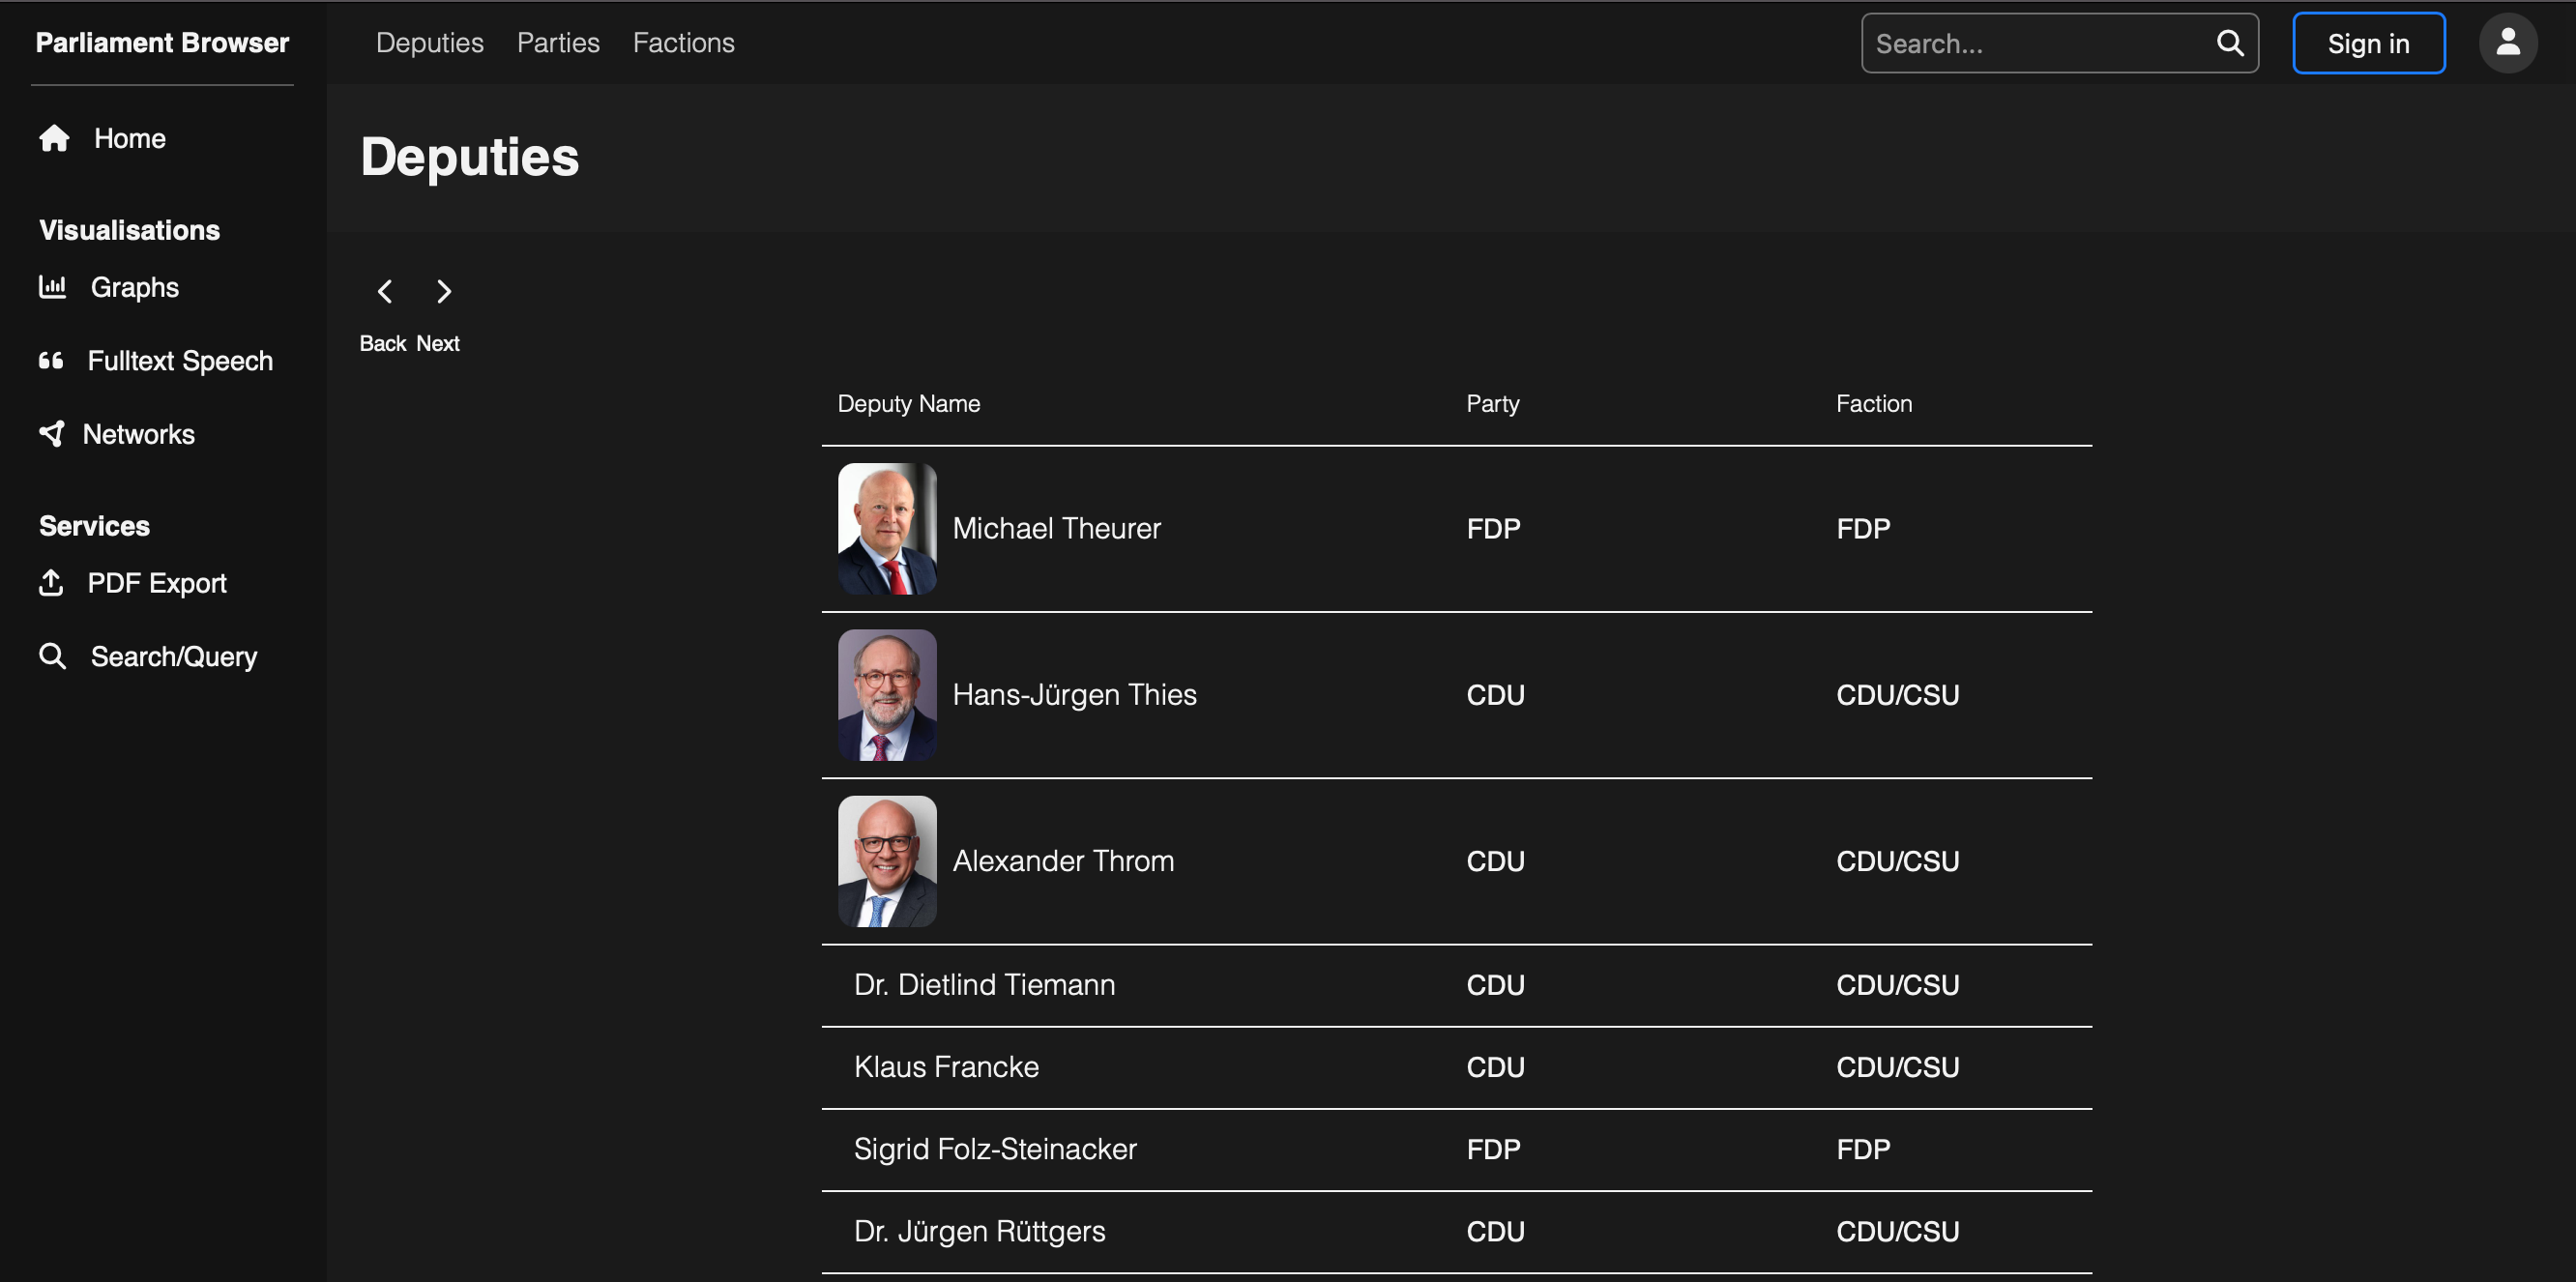
\includegraphics{deputies_page1}}
  	 \end{center}
	\caption{Deputies $\quad\rightarrow\quad$  Route:  /deputies}	
\end{figure}


\noindent Beim Klick auf den Namen des/der Abgeordneten stehen weitere Informationen über den/die Parlamentarier:in zur Verfügung. Persönliche Daten, welche auf den Bundestagsseiten zu finden sind, Angaben zur Vita und eine Auflistung aller Reden sind hier zu finden.  \\\\\\\\

\begin{figure}[H]
	\begin{center}		
		\scalebox{0.28}{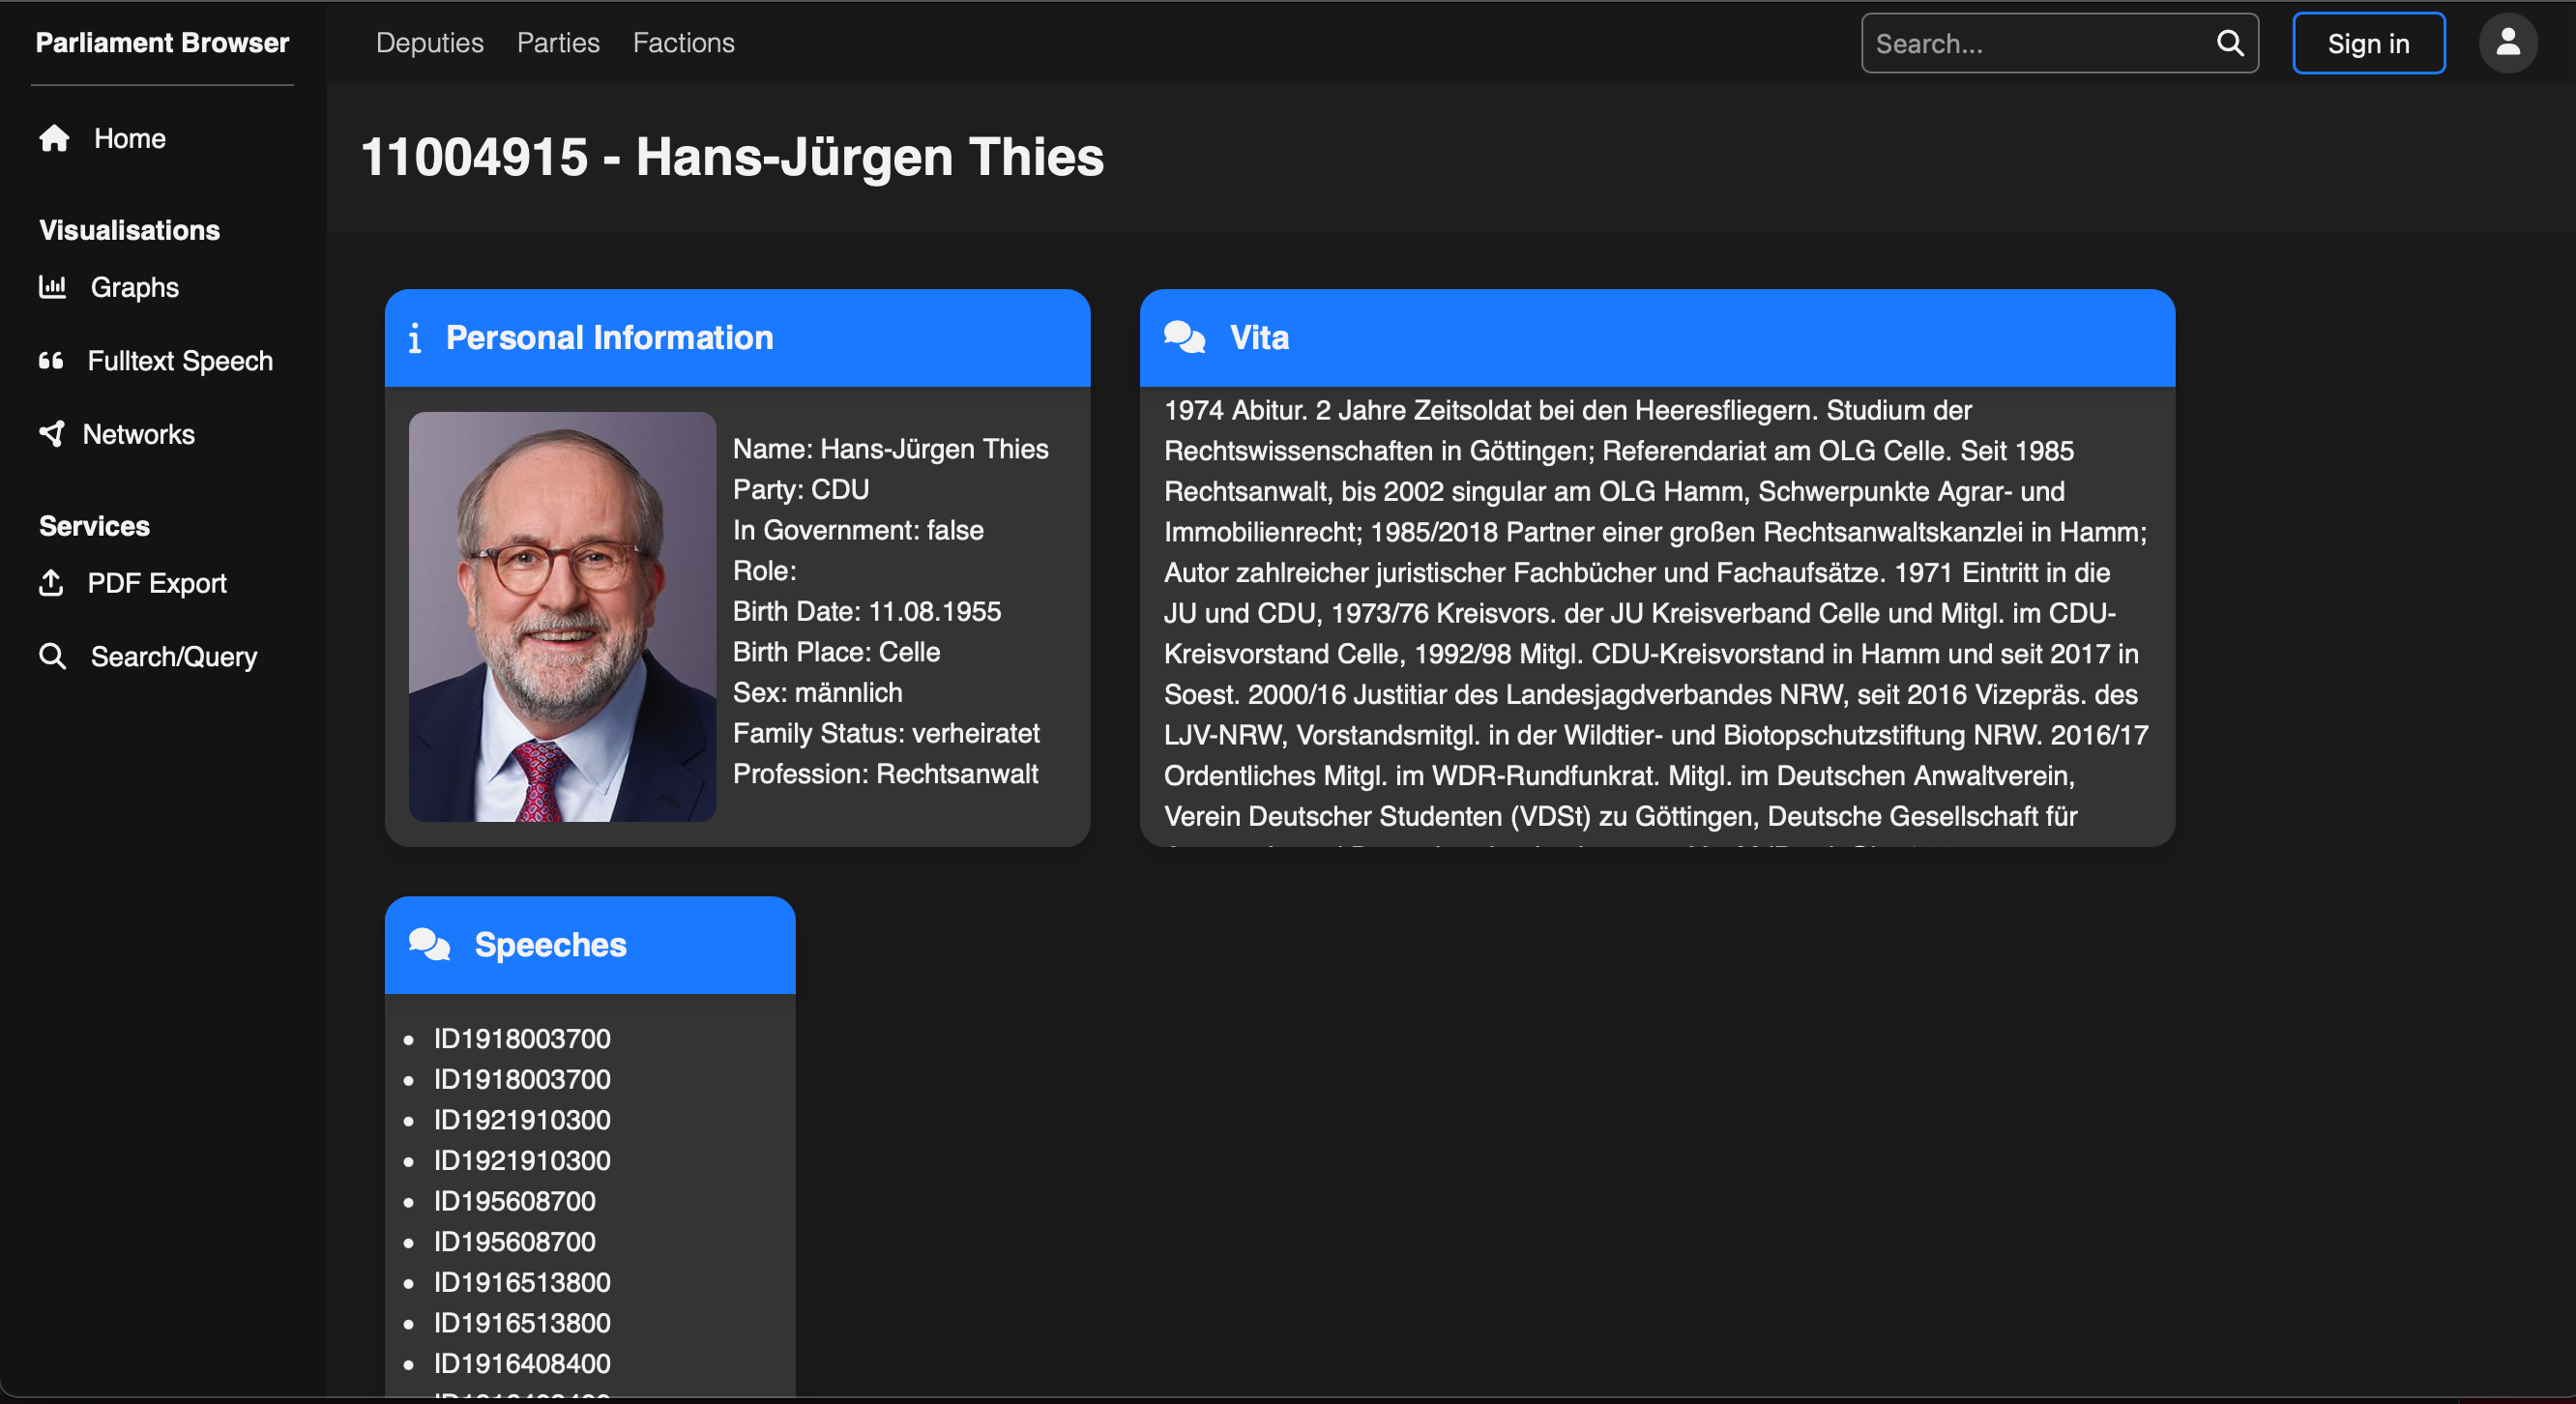
\includegraphics{deputies_page2}}
  	 \end{center}
	\caption{Deputies $\quad\rightarrow\quad$  Route:  /deputy?id=11001942}	
\end{figure}


\noindent Wie bei den oben aufgeführten Personen, führt ein Klick auf den Namen der Partei oder Fraktion zu mehr Angaben über eben diese Partei oder Fraktion. Zum Beispiel werden ihre Mitglieder vollständig aufgelistet. \\\\\\

\begin{figure}[H]
	\begin{center}		
		\scalebox{0.3}{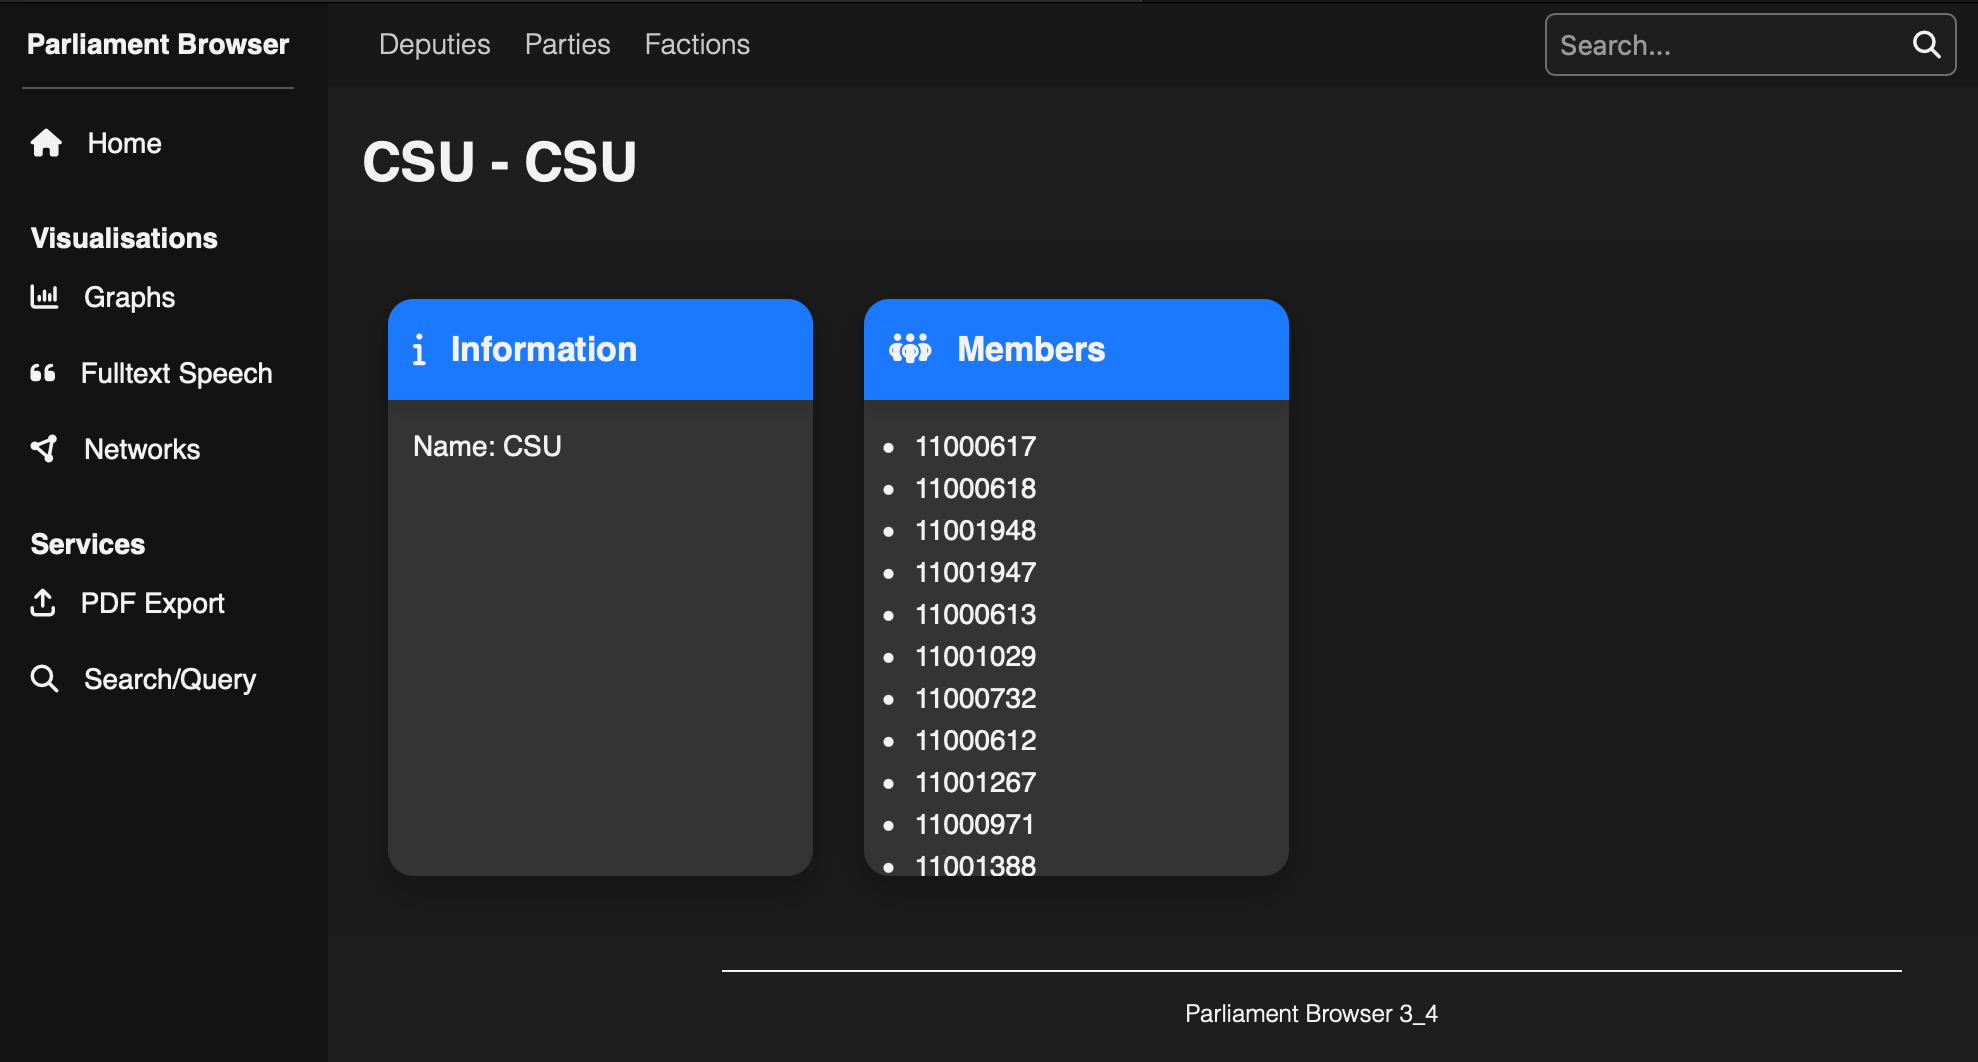
\includegraphics{deputies_page3}}
  	 \end{center}
	\caption{Deputies $\quad\rightarrow\quad$  Route:  /party?id=...}	
\end{figure}


\section{Parties $\quad\rightarrow\quad$  Route:  /parties}
Die Route $\,\rightarrow\,$ /parties, weiterhin in der oberen Navigationsleiste zu finden, führt zu einer Seite mit der Liste aller Parteien und ihren Mitgliedern. Über Letztere können wieder nähere Information über einen Klick erhalten werden.\\\\

\begin{figure}[H]
	\begin{center}		
		\scalebox{0.3}{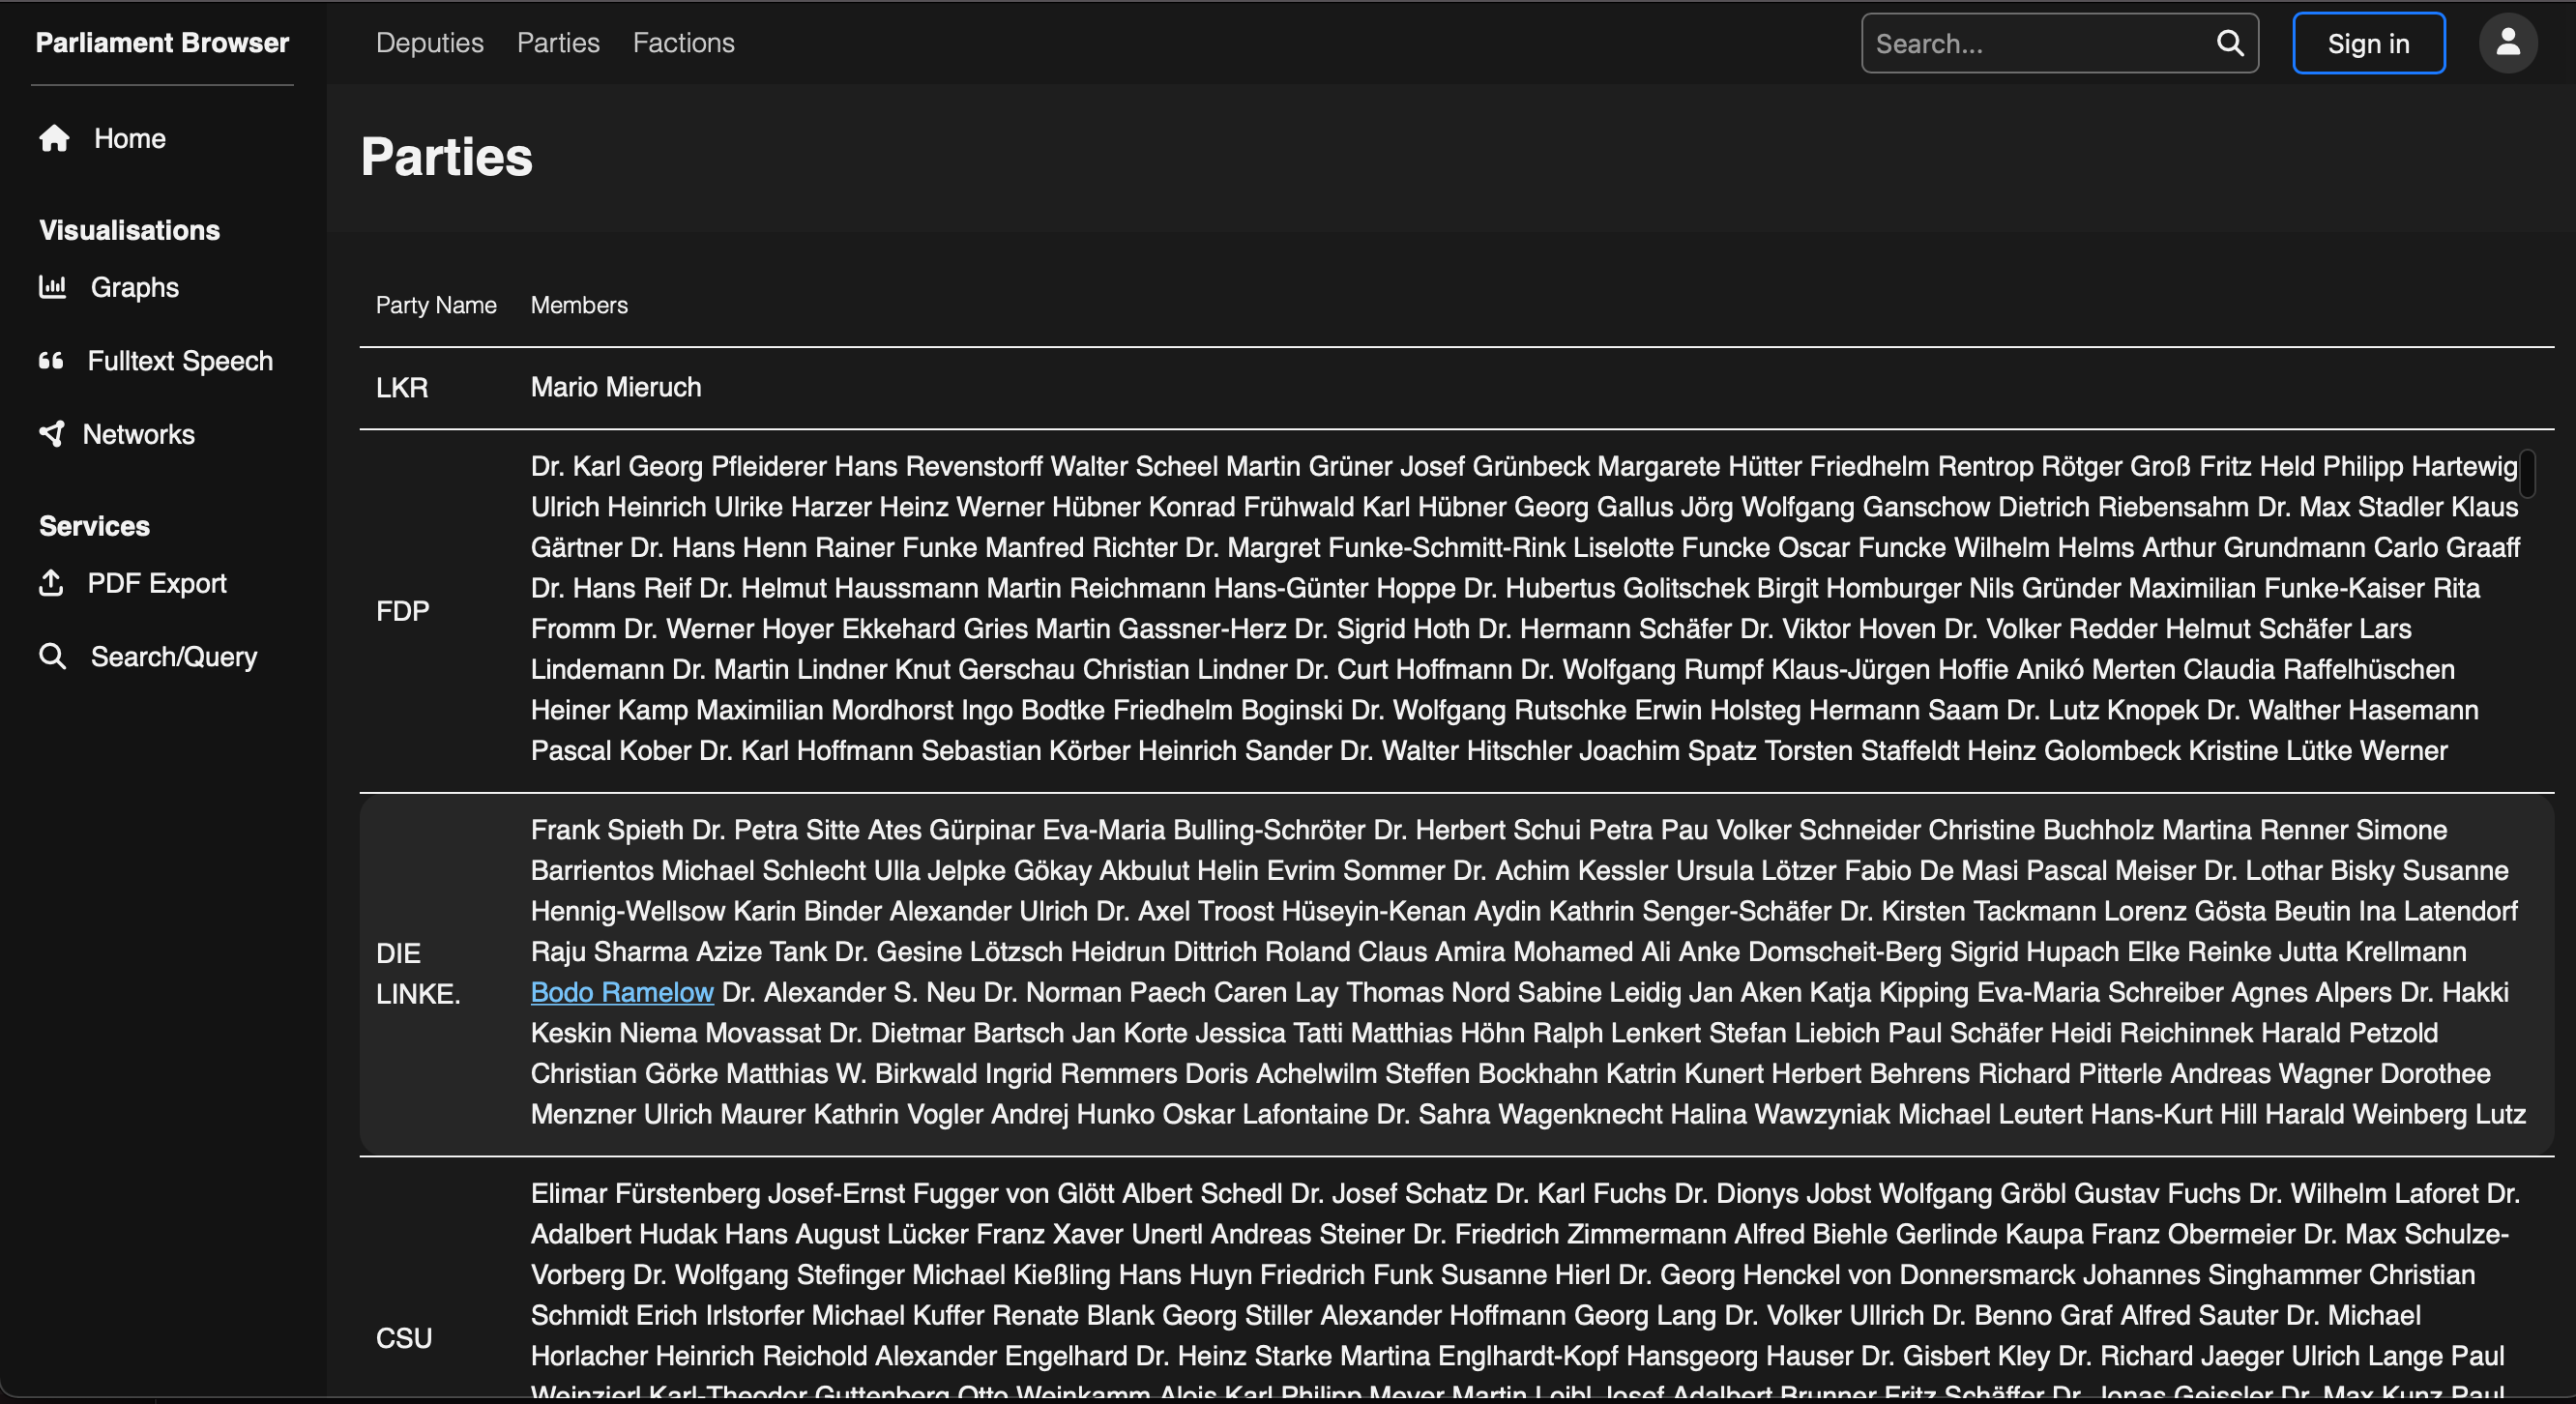
\includegraphics{parties_page1}}
  	 \end{center}
	\caption{Deputies $\quad\rightarrow\quad$  Route:  /parties}	
\end{figure}


\section{Factions $\quad\rightarrow\quad$  Route:  /factions}  
Auch bei den Fraktionen gilt, dass über eine Route, hier $\,\rightarrow\,$ /factions, nähere Informationen über die Fraktionen mit einem Klick erhalten werden können. Gleich rechts neben 'Parties' in der oberen Navigationsleiste ist sie als 'Factions' zu finden.\\\\

\begin{figure}[H]
	\begin{center}		
		\scalebox{0.3}{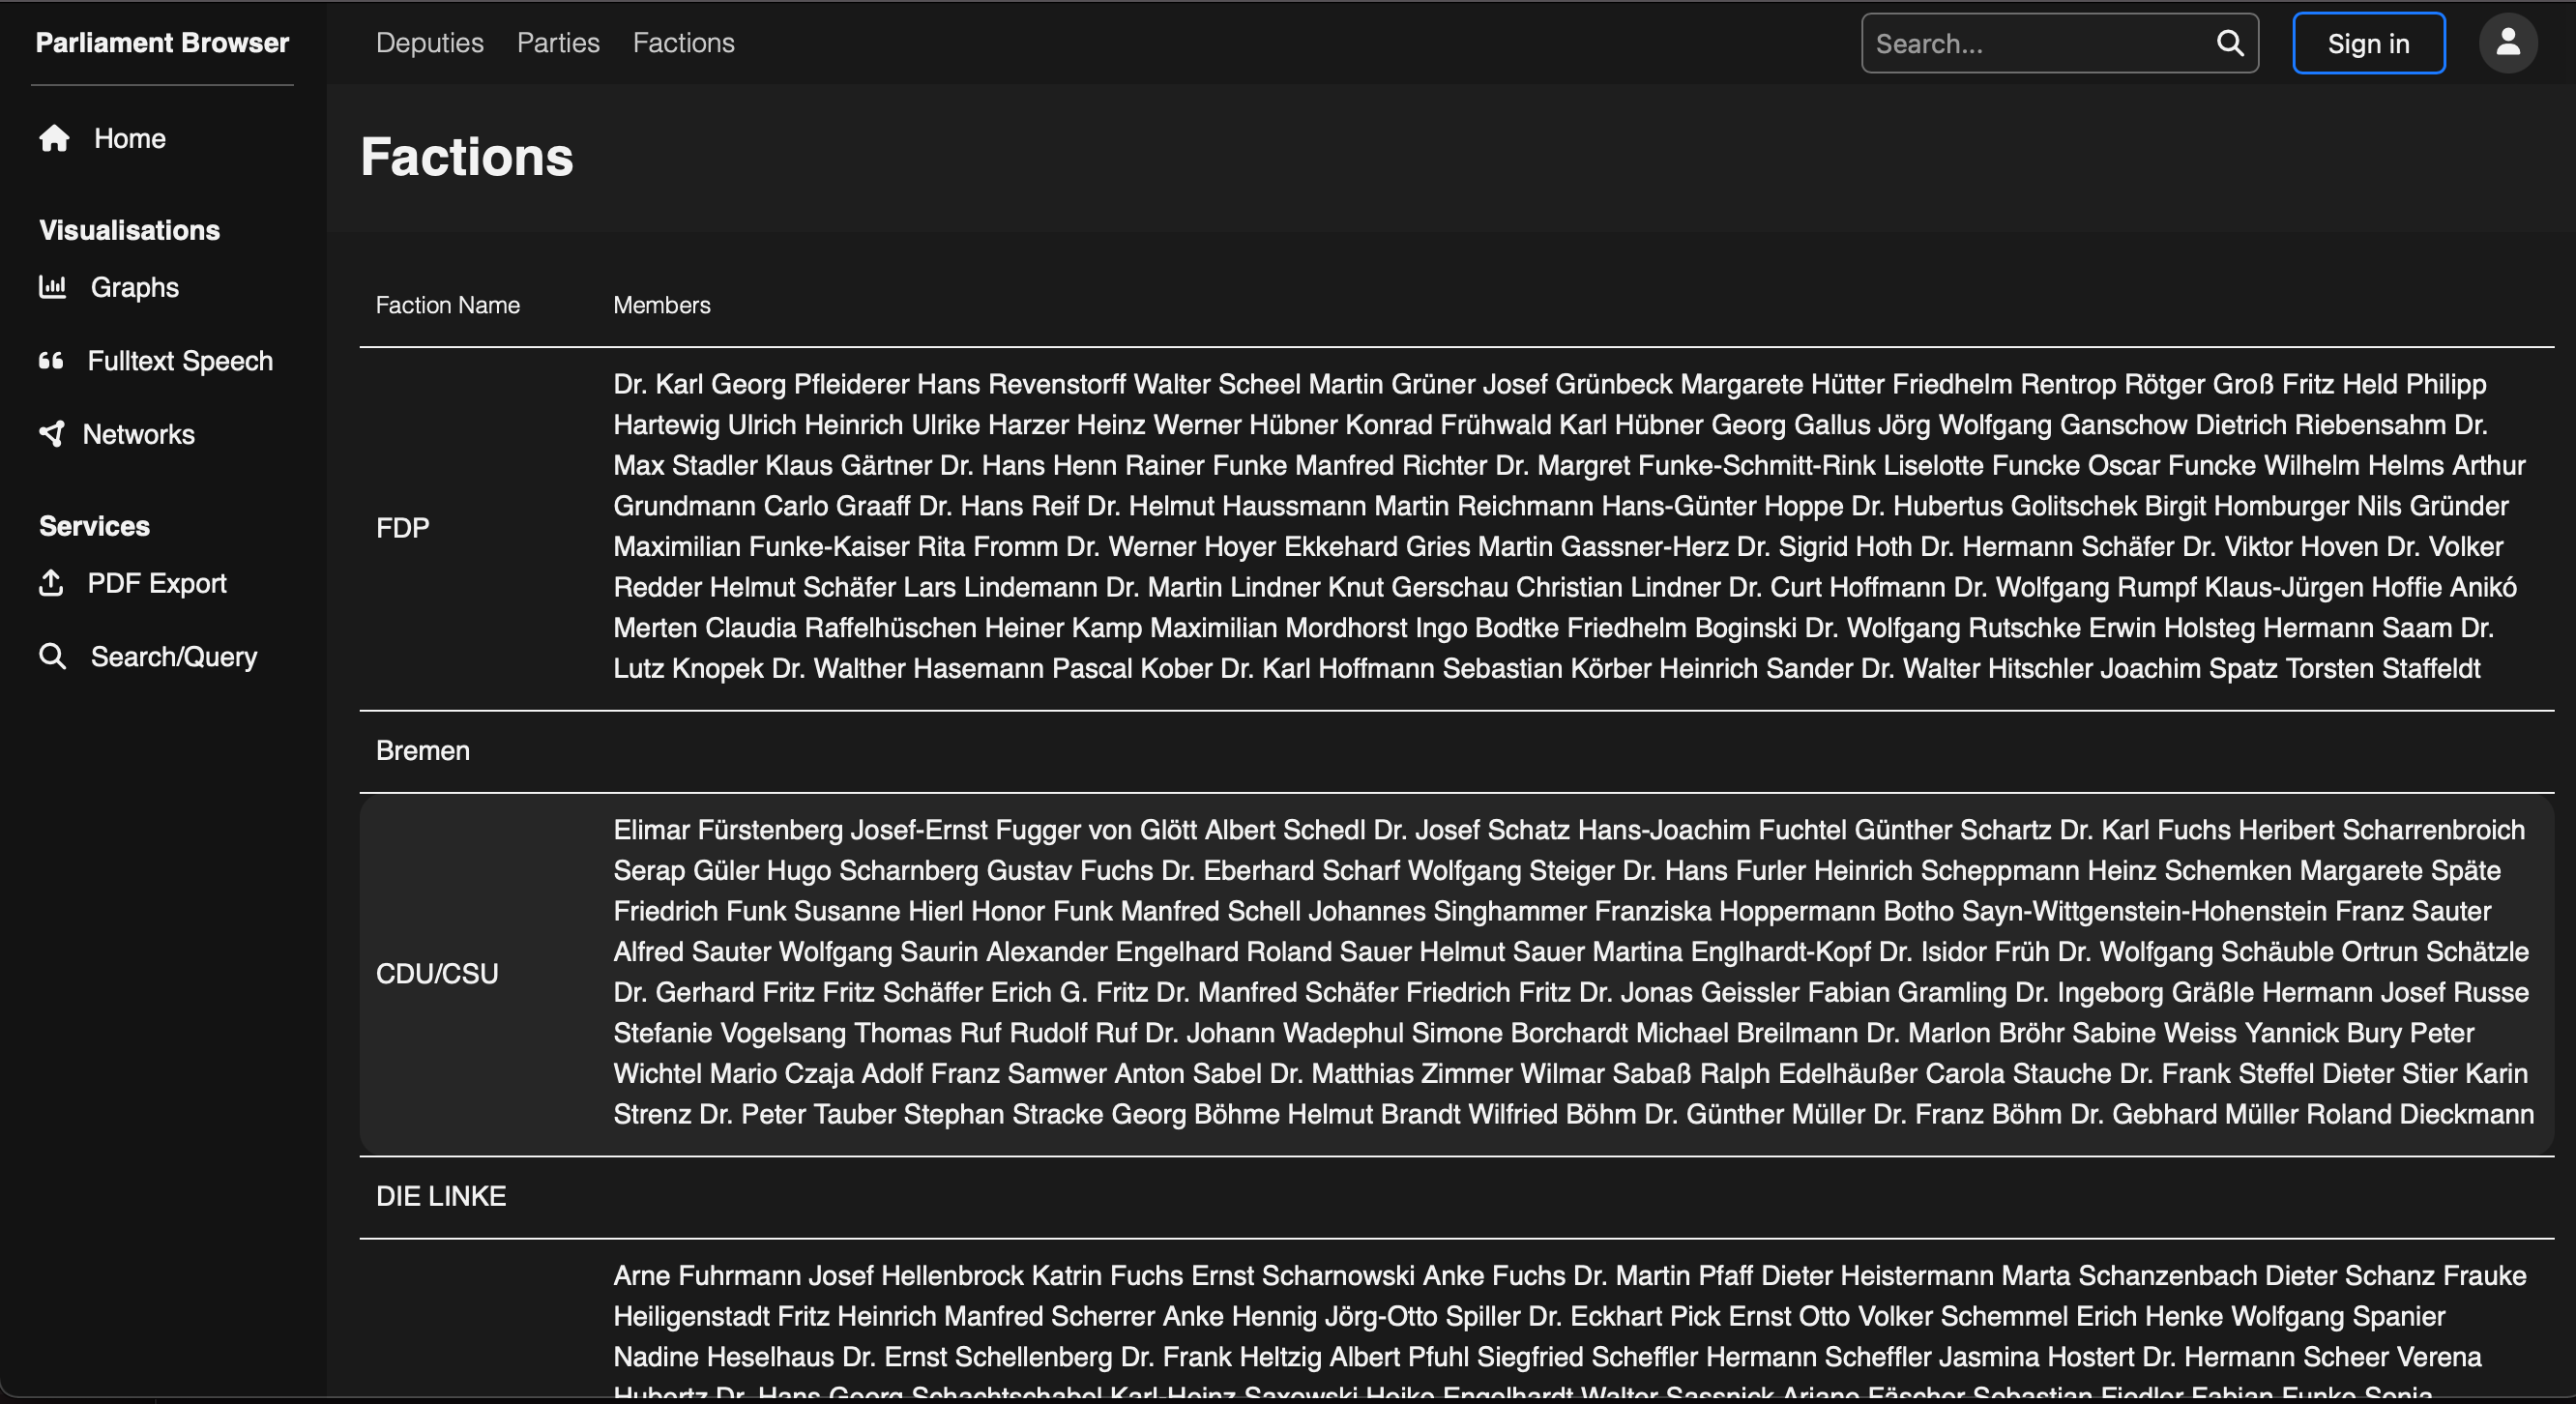
\includegraphics{factions_page1}}
  	 \end{center}
	\caption{Deputies $\quad\rightarrow\quad$  Route:  /factions}	
\end{figure}

\chapter{Visualisation}

Die folgenden Menüpunkte sind in der senkrechten Navigationsleiste links
gelistet. Visualisierungen und weitere Services, wie Latex PDF-Exporte oder Such-Queries sind hier vertreten.  

\section{Graphs $\quad\rightarrow\quad$  Route:  /graphs}
      
Unter dem Menüpunkt $Graphs$ findet man diverse Visualisierungen von NLP Annotationen. Alternativ, über sämtliche Reden oder gefiltert nach einem Zeitraum oder Suchbegriff.   \\
\noindent Die hier getroffene Auswahl von Annotationen sind nur ein kleiner Ausschnitt von möglichen NLP Analysen. Token, POS und NamedEntities stehen als Beispiel parat. Das Sentiment ist ein weitere Eigenschaft der NLP Analyse.  \\\\

     
\begin{figure}[H]
	\begin{center}		
		\scalebox{0.35}{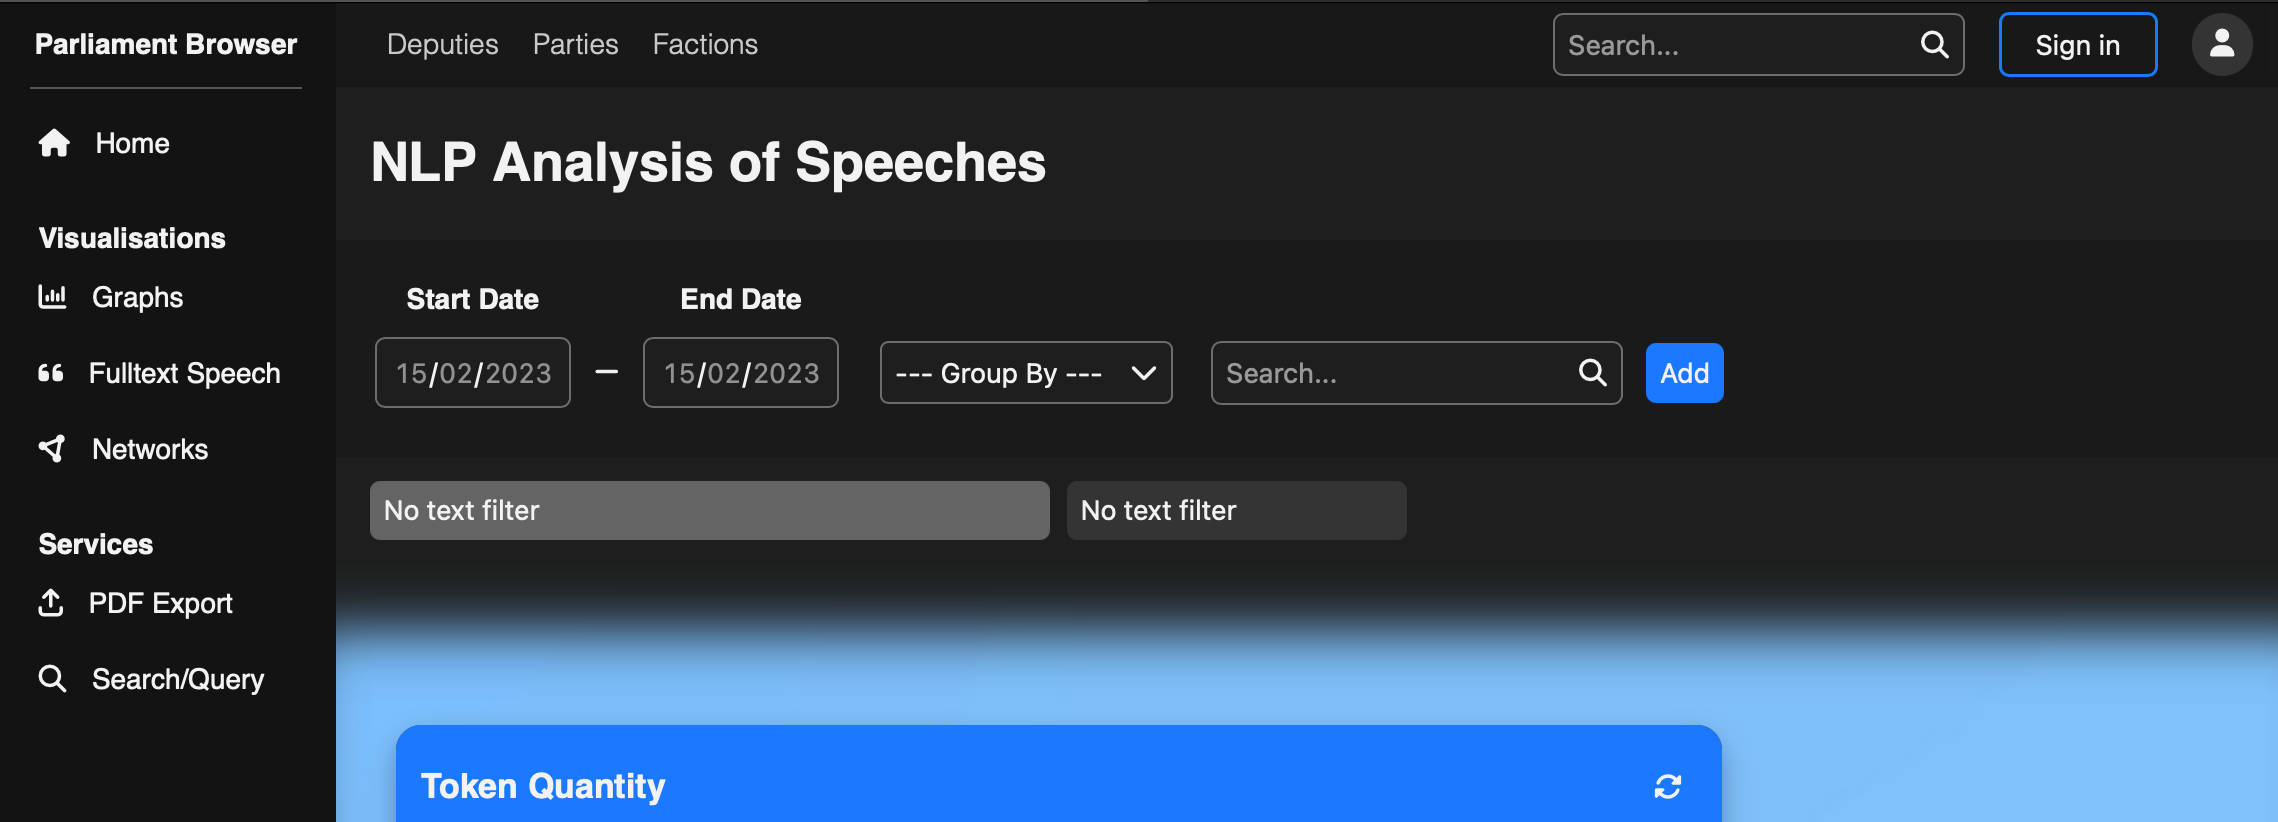
\includegraphics{graphs_page1}}
  	 \end{center}
	\caption{Graphs Site $\quad\rightarrow\quad$  Route:  /graphs}	
\end{figure}

\noindent Nach optionaler Eingabe eines $Start Date$ und $End Date$ sowie Suchbegriffs und Bestätigen mit $Add$, öffnet sich eines neues Tab-Panel 
und veranschaulicht in den folgenden Grafiken sämtliche Annotationen, beschränkt auf jene Reden, welche die Filterparameter erfüllen. (Idealerweise)\\\\
In das Feld $Search...$ können Suchbegriffe eingegeben werden, nach denen in den Reden gesucht wird. Per Filter sind in den Grafiken dann nur diese berücksichtigt. \\\\\\



\begin{figure}[H]
	\begin{center}		
		\scalebox{0.35}{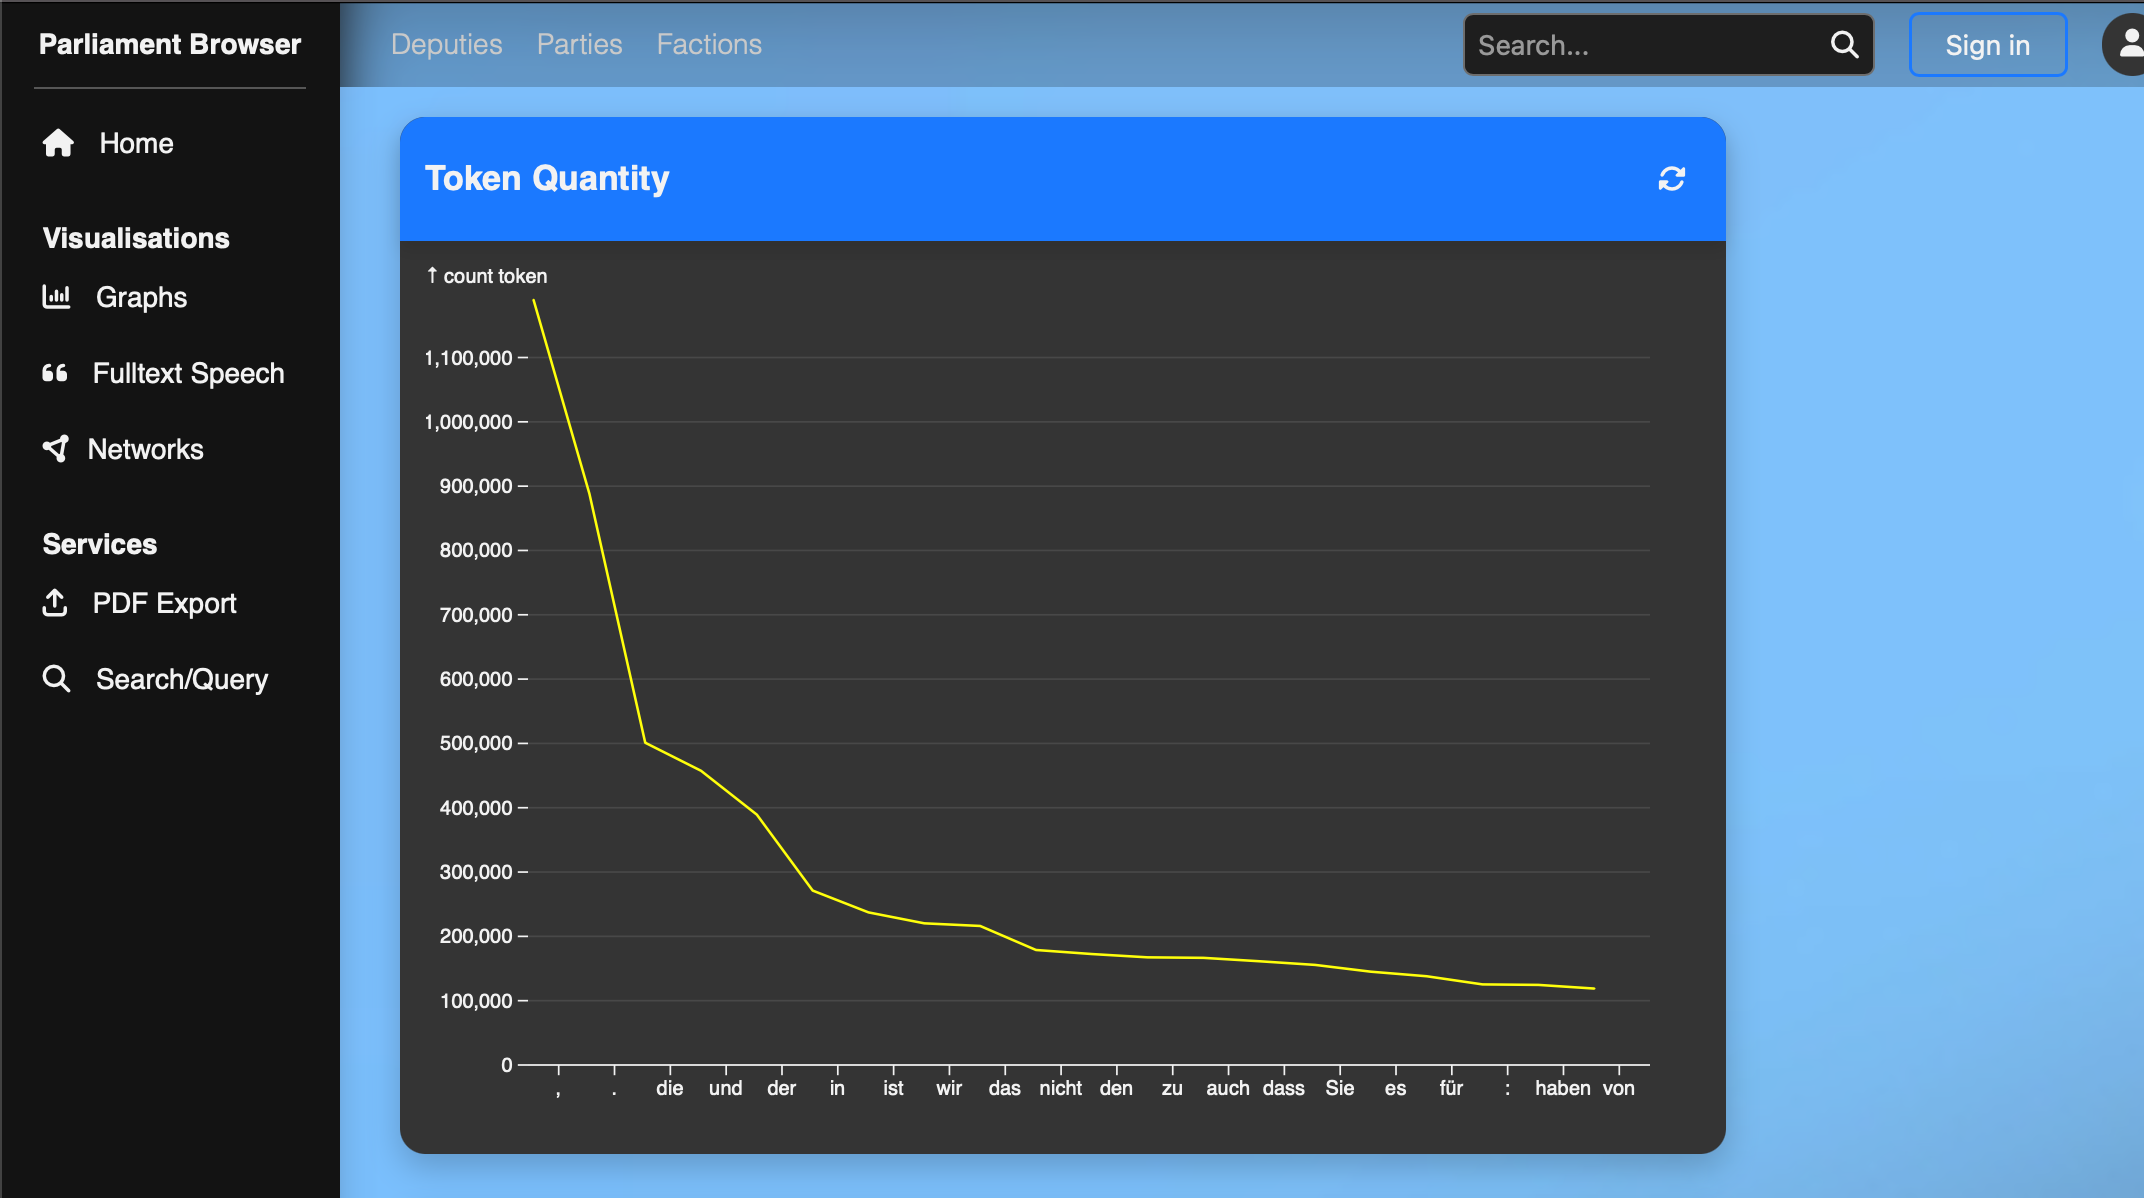
\includegraphics{graphs_page2}}
  	 \end{center}
	\caption{Token Distribution}	
\end{figure}


\noindent Als einführendes Beispiel kann die Häufigkeitsverteilung aller in den berücksichtigten Reden gefundenen $Token$ dienen. Zur besseren Illustration werden diese nach Prävalenz ihres Erscheinens sortiert. Wie erwartet sind Interpunktionszeichen, wie Komma und Punkt, die häufigsten Token. \\\\\\


\begin{figure}[H]
	\begin{center}		
		\scalebox{0.35}{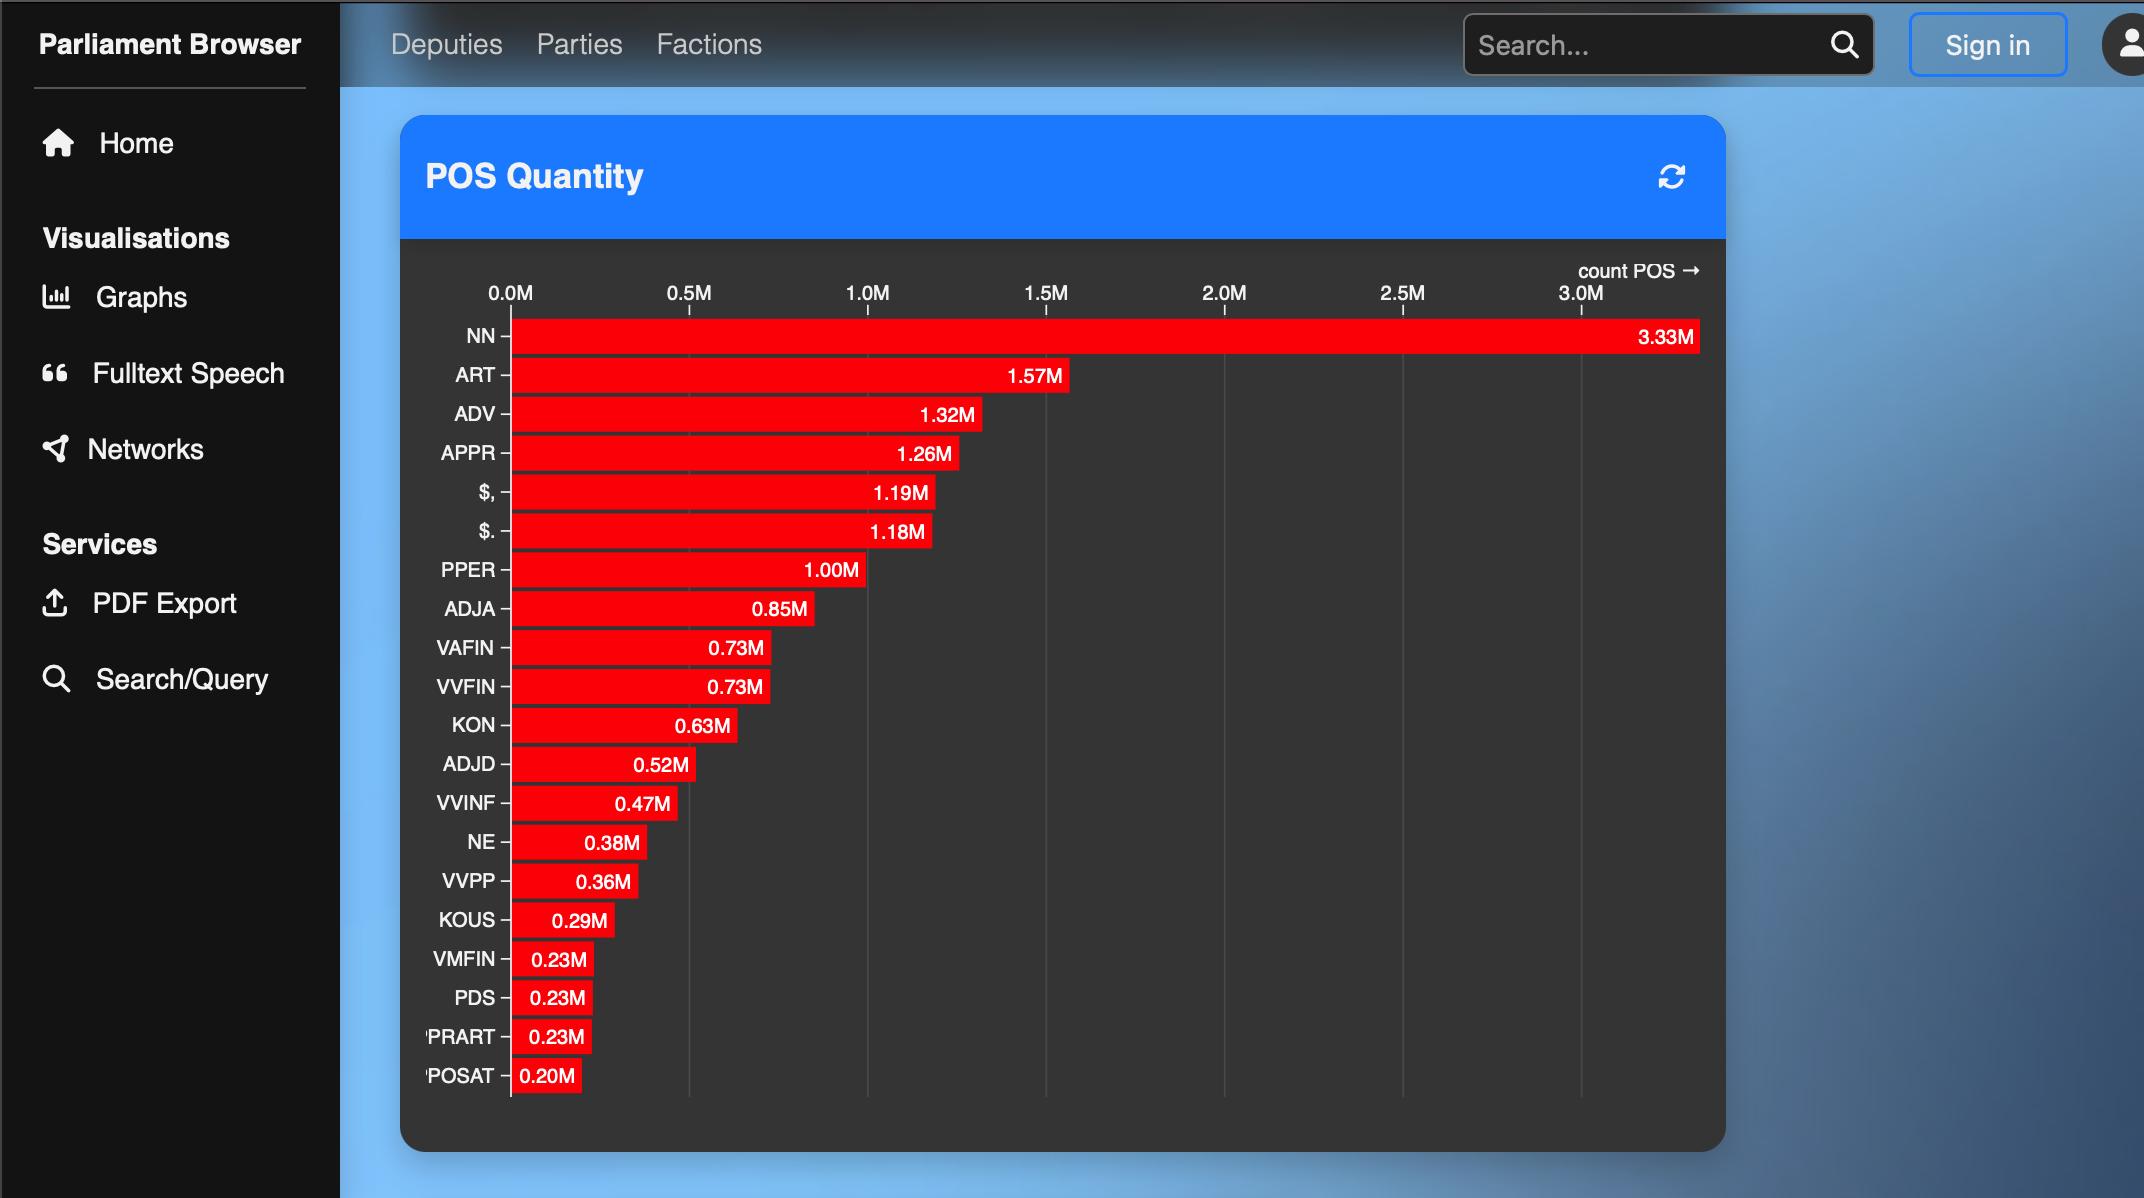
\includegraphics{graphs_page3}}
  	 \end{center}
	\caption{POS  Distribution}	
 \end{figure}

\noindent Als nächstes Beispiel, die Häufigkeitsverteilung aller in den berücksichtigten Reden gefundenen Parts of Speech, oder abgekürzt $POS$. Auch hier wird zur besseren Illustration  nach Prävalenz des Erscheinens sortiert. Diesmal als horizontaler BarChart dargestellt, erkennt man, dass Substantive, eines der N steht für Noun, die häufigsten Bausteine, parts of speech, der deutschen Sprache sind. Zumindest in diesem Corpus der Bundestagsdebatten.\\\\

\noindent Es folgt die Häufigkeitsverteilung des Sentiments in den jeweiligen Reden, welche per Filter Berücksichtigung finden. \\\\\\\\
\begin{figure}[H]
	\begin{center}		
		\scalebox{0.5}{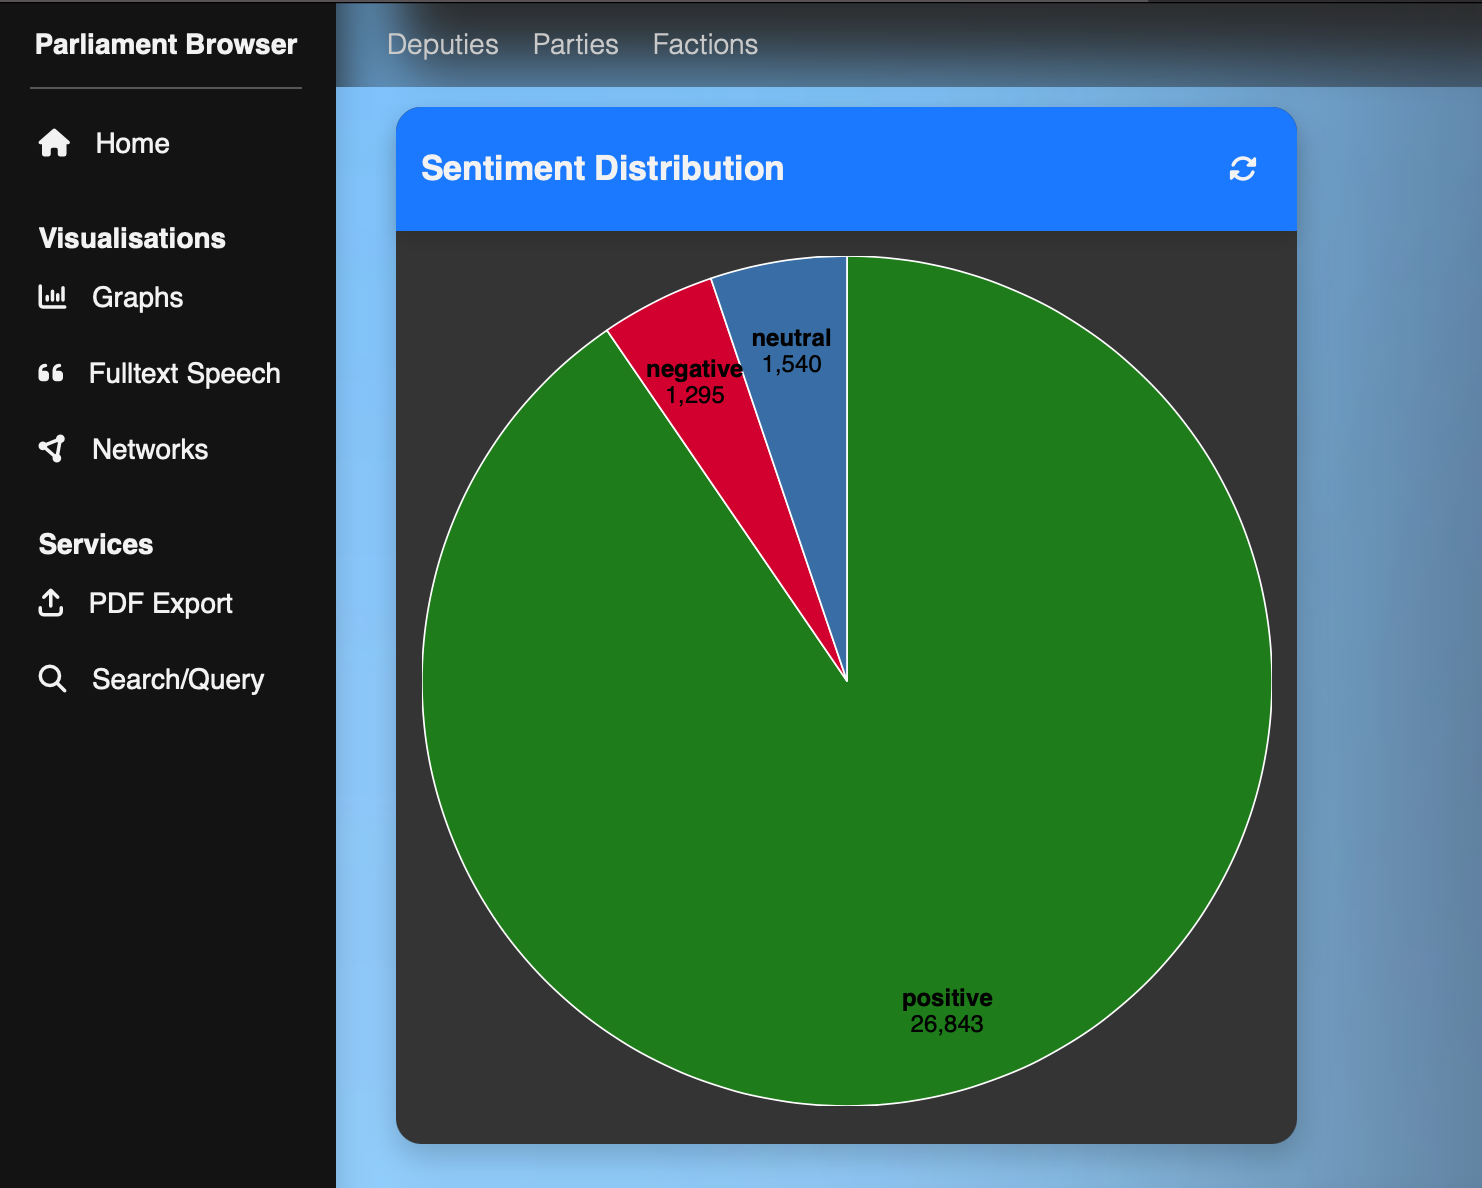
\includegraphics{graphs_page4}}
  	 \end{center}
	\caption{Sentiment  Distribution}	
 \end{figure}



\begin{figure}[H]
	\begin{center}		
		\scalebox{0.35}{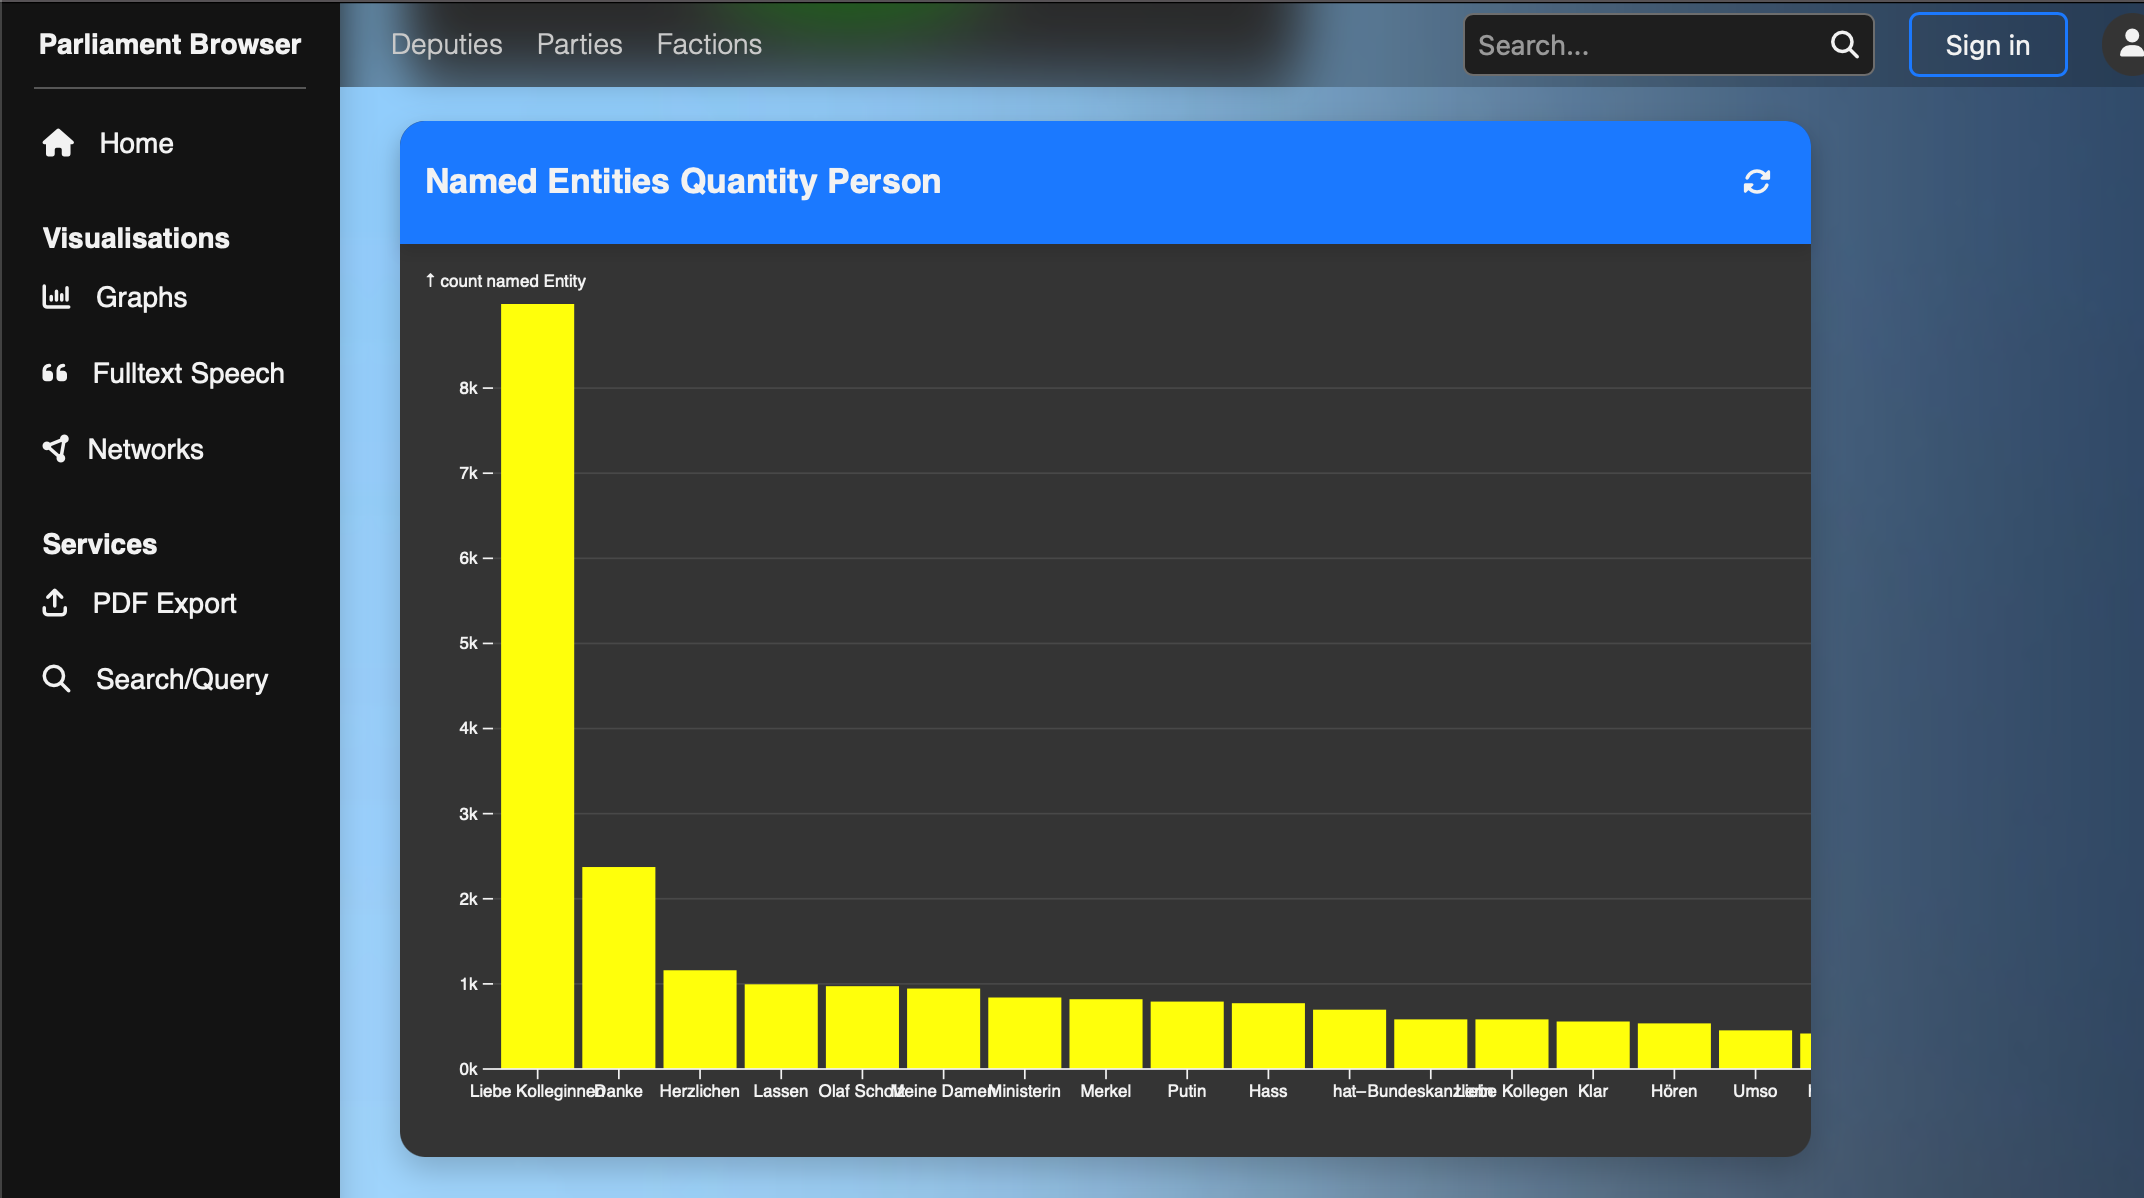
\includegraphics{graphs_page5}}
  	 \end{center}
	\caption{Named Entities Distribution Person}	
 \end{figure}


\noindent Die Auflistung der Named Entities, ebenfalls nach Häufigkeit sortiert, unterscheiden wir nach Named Entities von Personen, ... \\\\\\


\begin{figure}[H]
	\begin{center}		
		\scalebox{0.35}{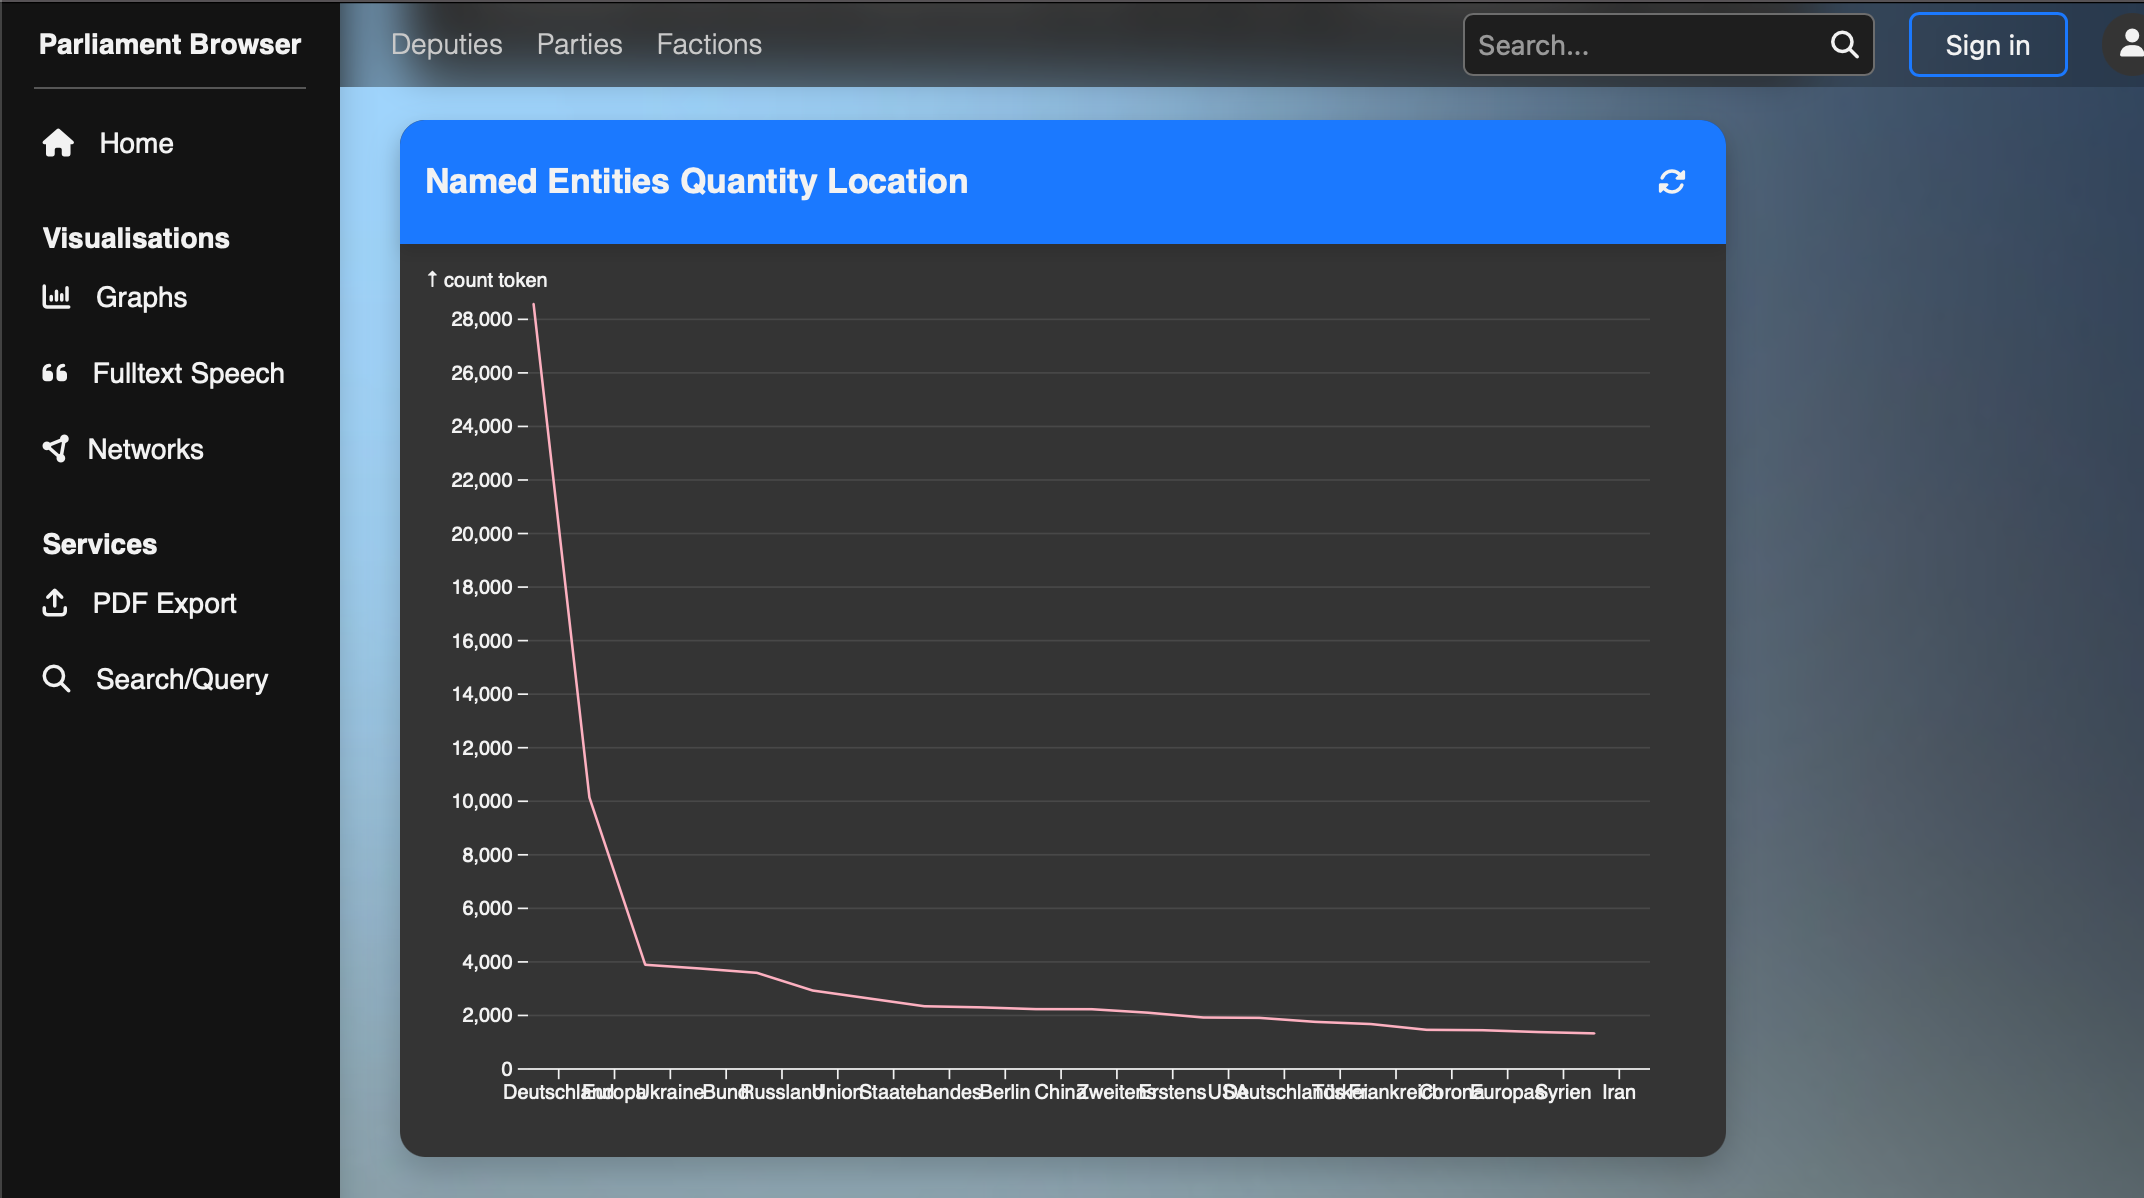
\includegraphics{graphs_page6}}
  	 \end{center}
	\caption{Named Entities Distribution Location}	
 \end{figure}


\noindent Named Entities von Lokationen und schliesslich ...\\\\\\


\begin{figure}[H]
	\begin{center}		
		\scalebox{0.35}{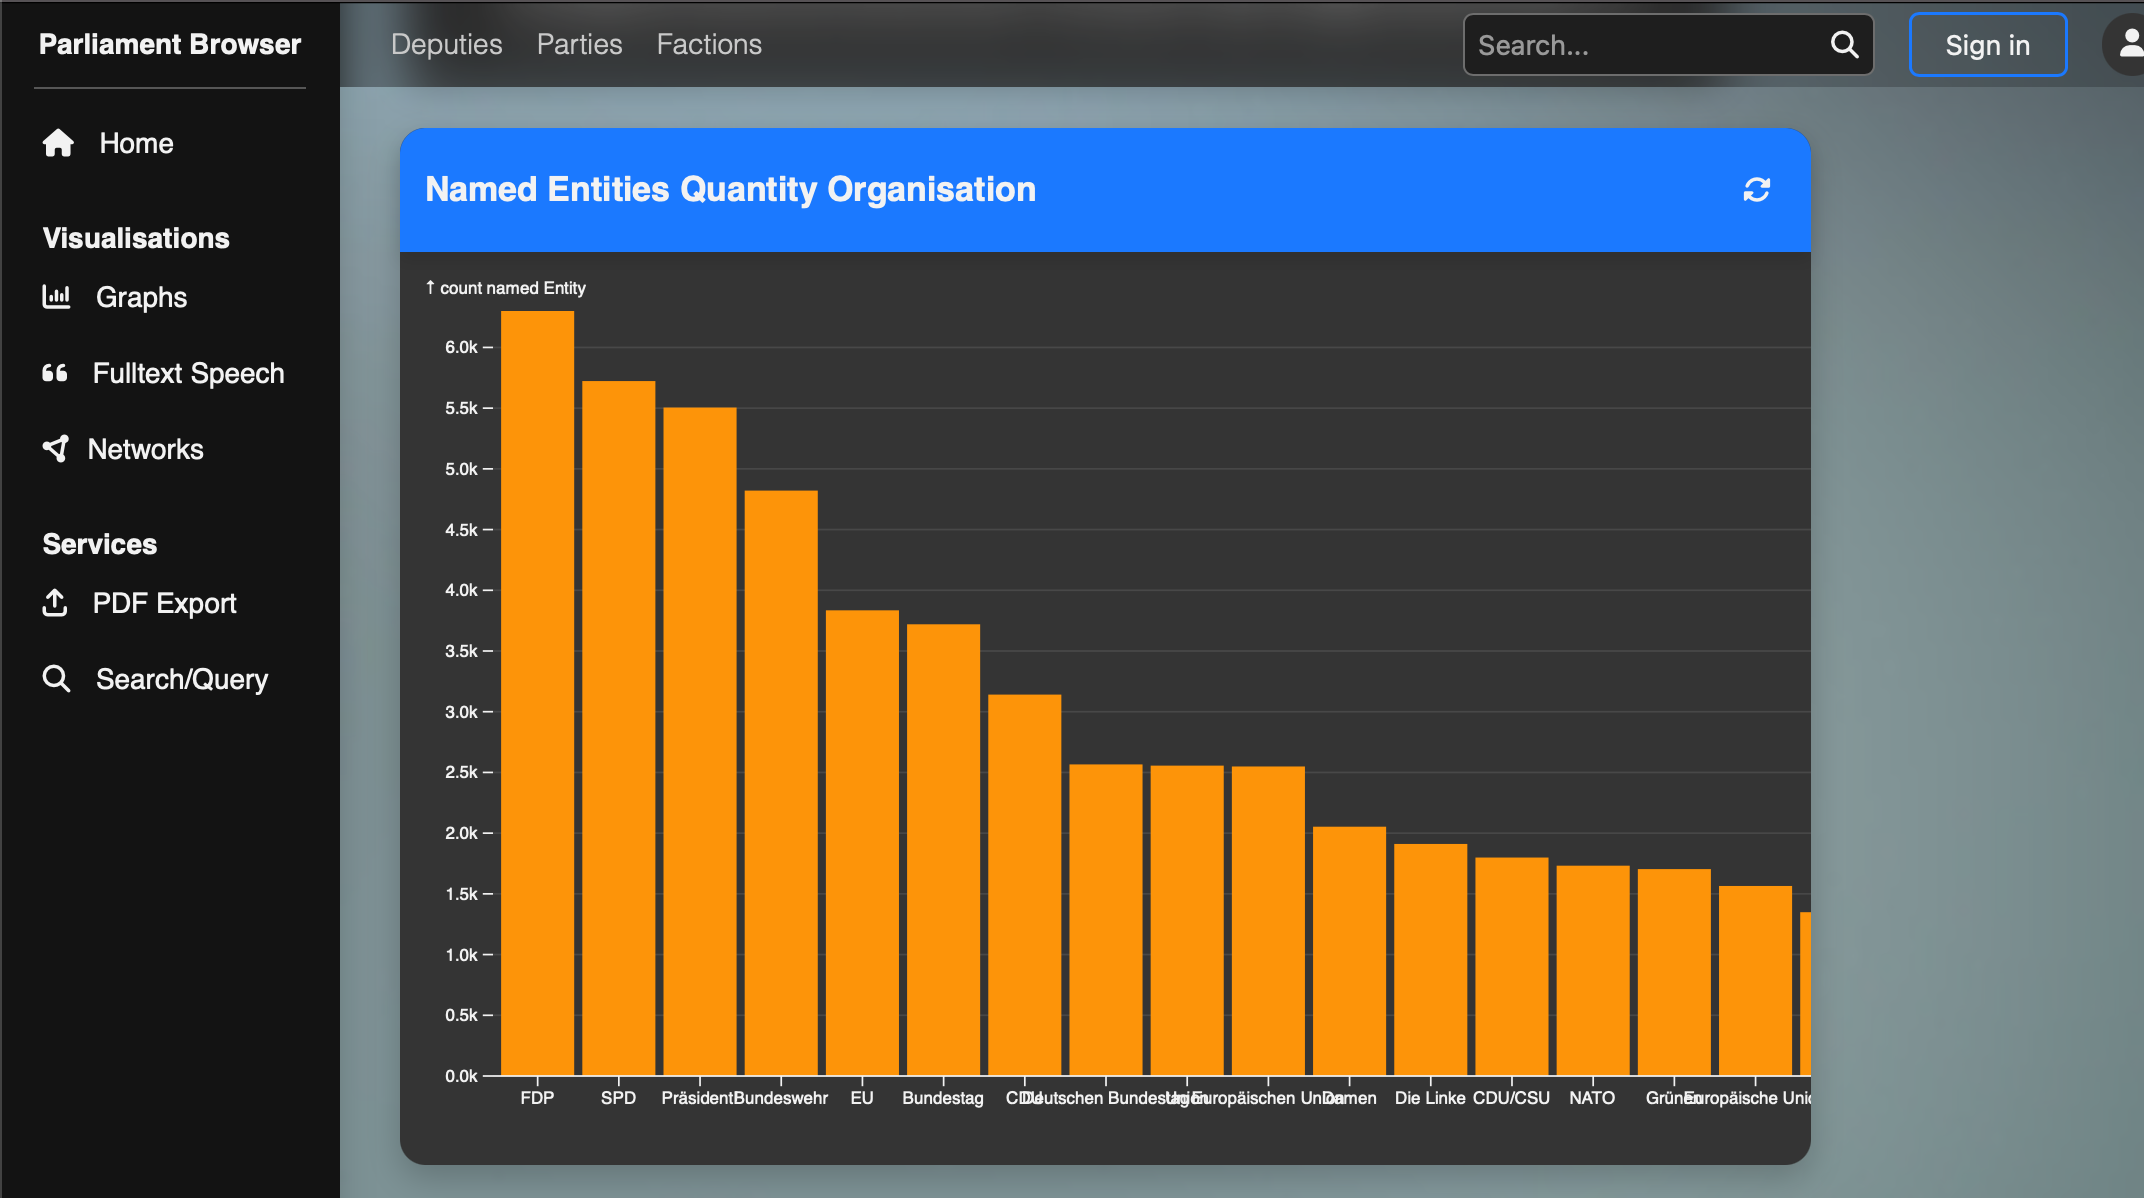
\includegraphics{graphs_page7}}
  	 \end{center}
	\caption{Named Entities Distribution Organisation}	
 \end{figure}


\noindent Named Entities von Organisationen. \\

\noindent Token, POS und NamedEntities sind nur ein paar wenige Beispiele von Annotationen, die man nach aufwendigen Natural Language Processing Analysen gewinnen kann. Mühelos könnten weitere linguistische Bausteine und Konzepte bereitgestellt und graphisch zur Illustration aufbereitet werden. \\

\noindent Als letzte Veranschaulichung diene die Häufigkeitsverteilung der Anzahl der Reden eines Redners, welcher in den berücksichtigten Reden als solcher erkannt wird, $Speaker Distribution$. \\\\
 
 \begin{figure}[H]
	\begin{center}		
		\scalebox{0.35}{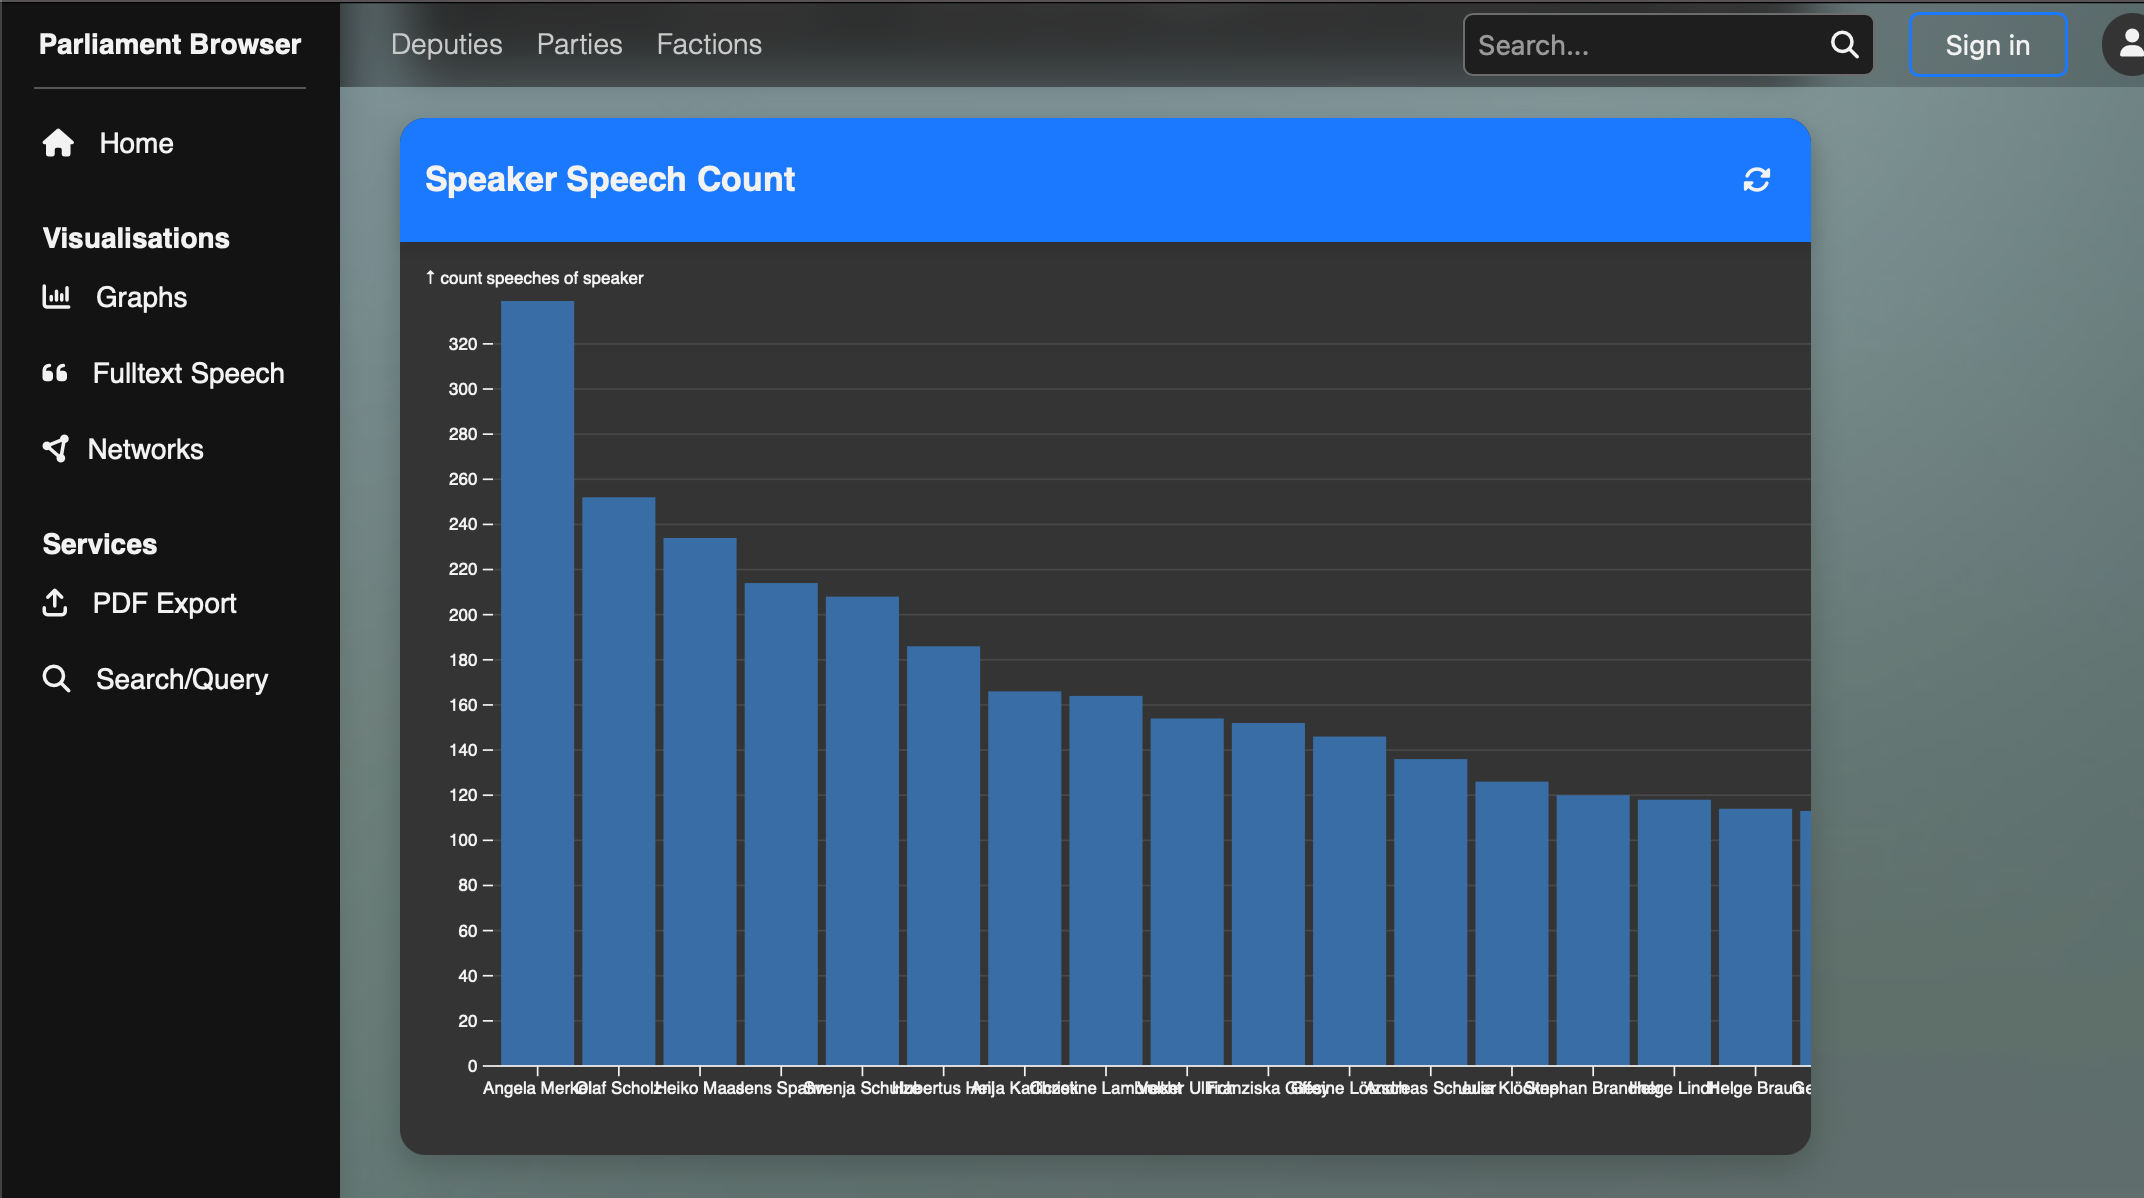
\includegraphics{graphs_page8}}
  	 \end{center}
	\caption{Speaker Distribution}	
 \end{figure}


\section{Fulltext  $\quad\rightarrow\quad$  Route:  /fulltextSpeechSite}    
In der $Fulltext Speech$ Analyse wird der Redetext einer vollständigen Rede dargestellt und Annotationen farblich illustriert. 
Die Identifikation der Rede erfolgt mit der, von Bundesbehörden verliehenen, offiziellen ID. 
Der vollständige Name des Redners, Partei- und Fraktionszugehörigkeit wird aufgeführt, und - falls vorhanden - ein Bild des Redners. 
Die aus der NLP Analyse gewonnenen Named Entity Annotations kommen hier noch einmal zur Geltung.
Mit der Farbe Orange werden per NLP Analyse erkannte Personen markiert. 
Grün dient der Kennzeichnung der im Text identifizierten Örtlichkeiten/Lokationen. 
Im Text namentlich erwähnte Organisationen werden violett hervorgehoben.
Außerdem wird das Sentiment jedes Satzes in einem blauen Label hinter dem jeweiligen Satz angezeigt.
Unterhalb der Rede werden zuletzt die Kommentare aufgeführt.\\\\ 
Mittels eines Aufklapp-Menüs auf der linken Seite können Protokolle, Tagesordnungspunkte und schließlich Reden ausgewählt werden.\\\\

\begin{figure}[H]
	\begin{center}		
		\scalebox{0.3}{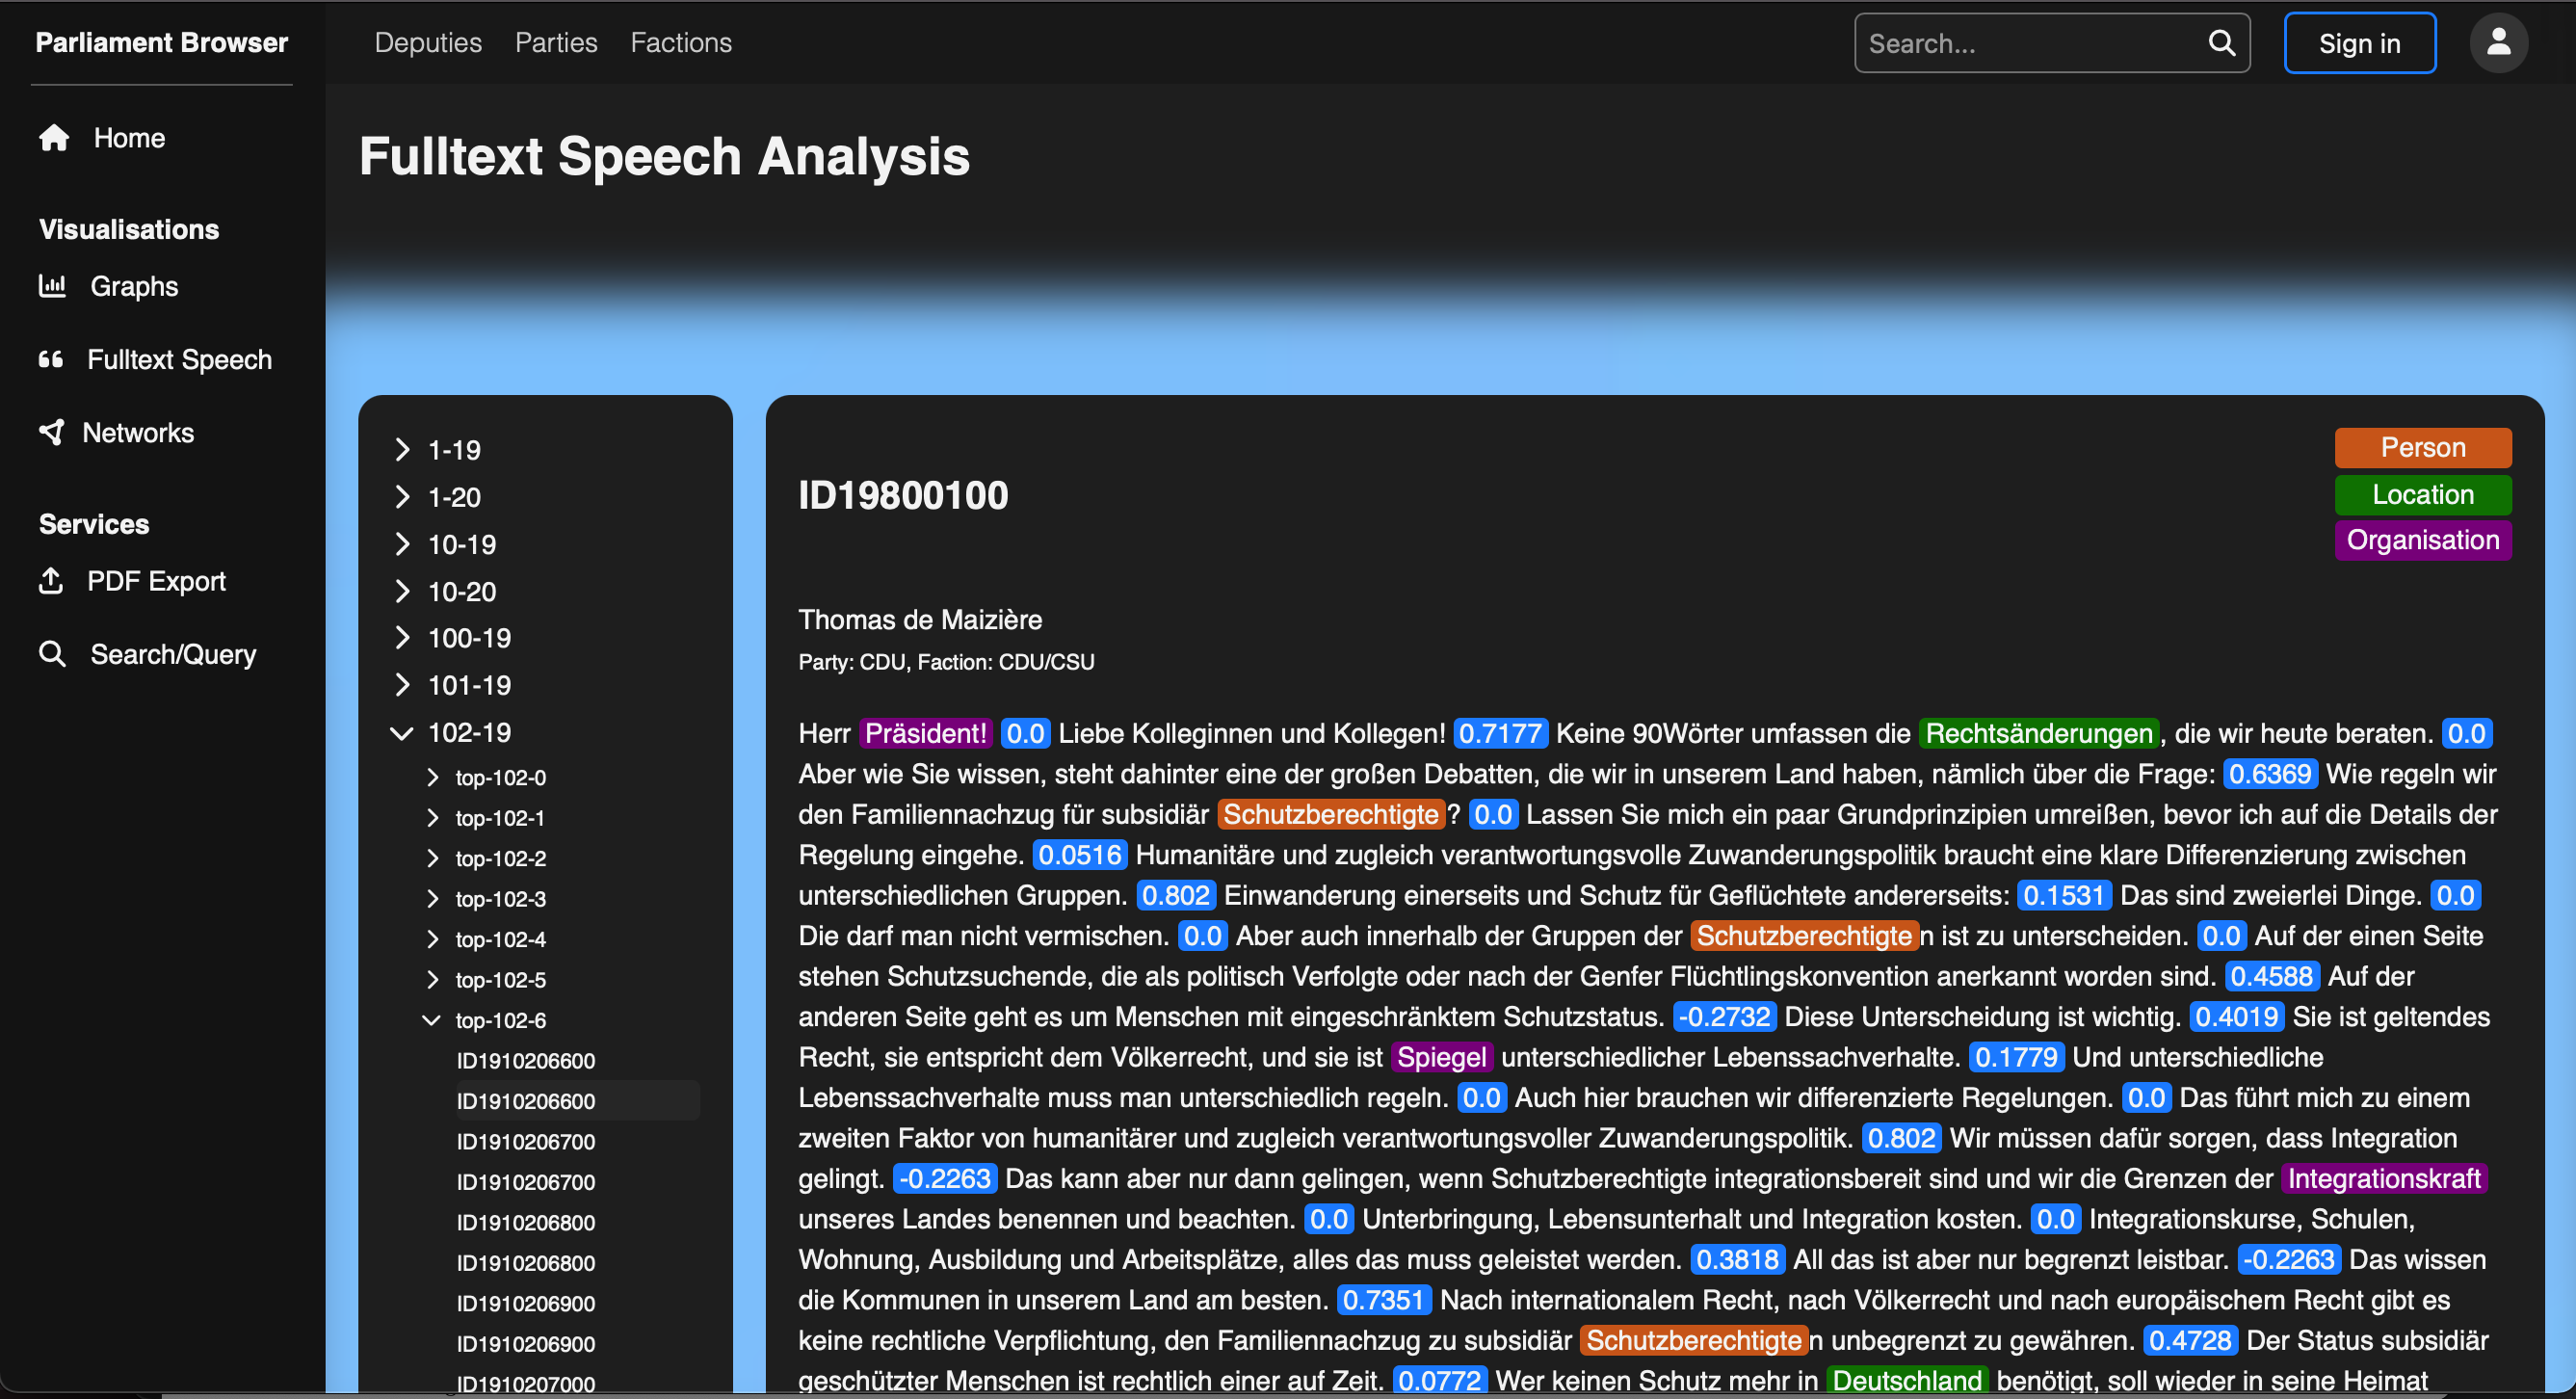
\includegraphics{fulltext_page1}}
  	 \end{center}
	\caption{Fulltext Speech Analysis}	
 \end{figure}

\pagebreak

\section{Networks}

Netzwerke sind ein interessantes und informatives Werkzeug, um Zusammenhänge und/oder Abhängigkeiten diverser Variablen einer komplexen Struktur aufzudecken. 
Die Visualisierung dieser Interdependenzen offenbart verborgene Relationen, aus denen nützliche  Erkenntnisse gewonnen werden können.\\\\
Das Kommentar-Netzwerk (Route $\quad\rightarrow\quad$  /commentNetwork) ist ein solches. Es veranschaulicht graphisch, welche Redner:innen von welchen Abgeordneten:innen kommentiert wurden. 
Dabei wird auch das Sentiment als Farbe der Kante visualisiert. Eine rote Kante symbolisiert einen eher negativen Kommentar, eine blaue einen neutralen Beitrag, während grün für eine positive Äusserung steht.
Je dicker und länger eine Kante ist, desto häufiger wurde kommentiert.
Mit dem Parameter $Sample Size$ kann ausgewählt werden, wie viele Kommentare bei dieser Anaylse miteinbezogen werden sollen. Aufgrund langer Laufzeit ist ein Standardwert von 1000 Kommentaren festgelegt.
Die $Minimum Comment Frequency$ gibt an, wie häufig ein Abgeordneter einen anderen Abgeordneten mindestens kommentiert haben muss, damit diese Relation angezeigt wird.
Achtung! Eine niedrige Comment Frequency und eine hohe Sample Size führen zu einer massiven Anzahl an Knoten und Kante im Netzwerk und wirken sich möglicherweise negativ auf die Performance der Website aus.\\\\ 
Mit der Maus kann außerdem der sichtbare Bereich des Netzwerks, sowie die dynamische Position der Knoten beeinflusst werden, ähnlich zu einer Karte. Dies trifft auf alle Netzwerke zu.\\\\

\begin{figure}[H]
	\begin{center}		
		\scalebox{0.4}{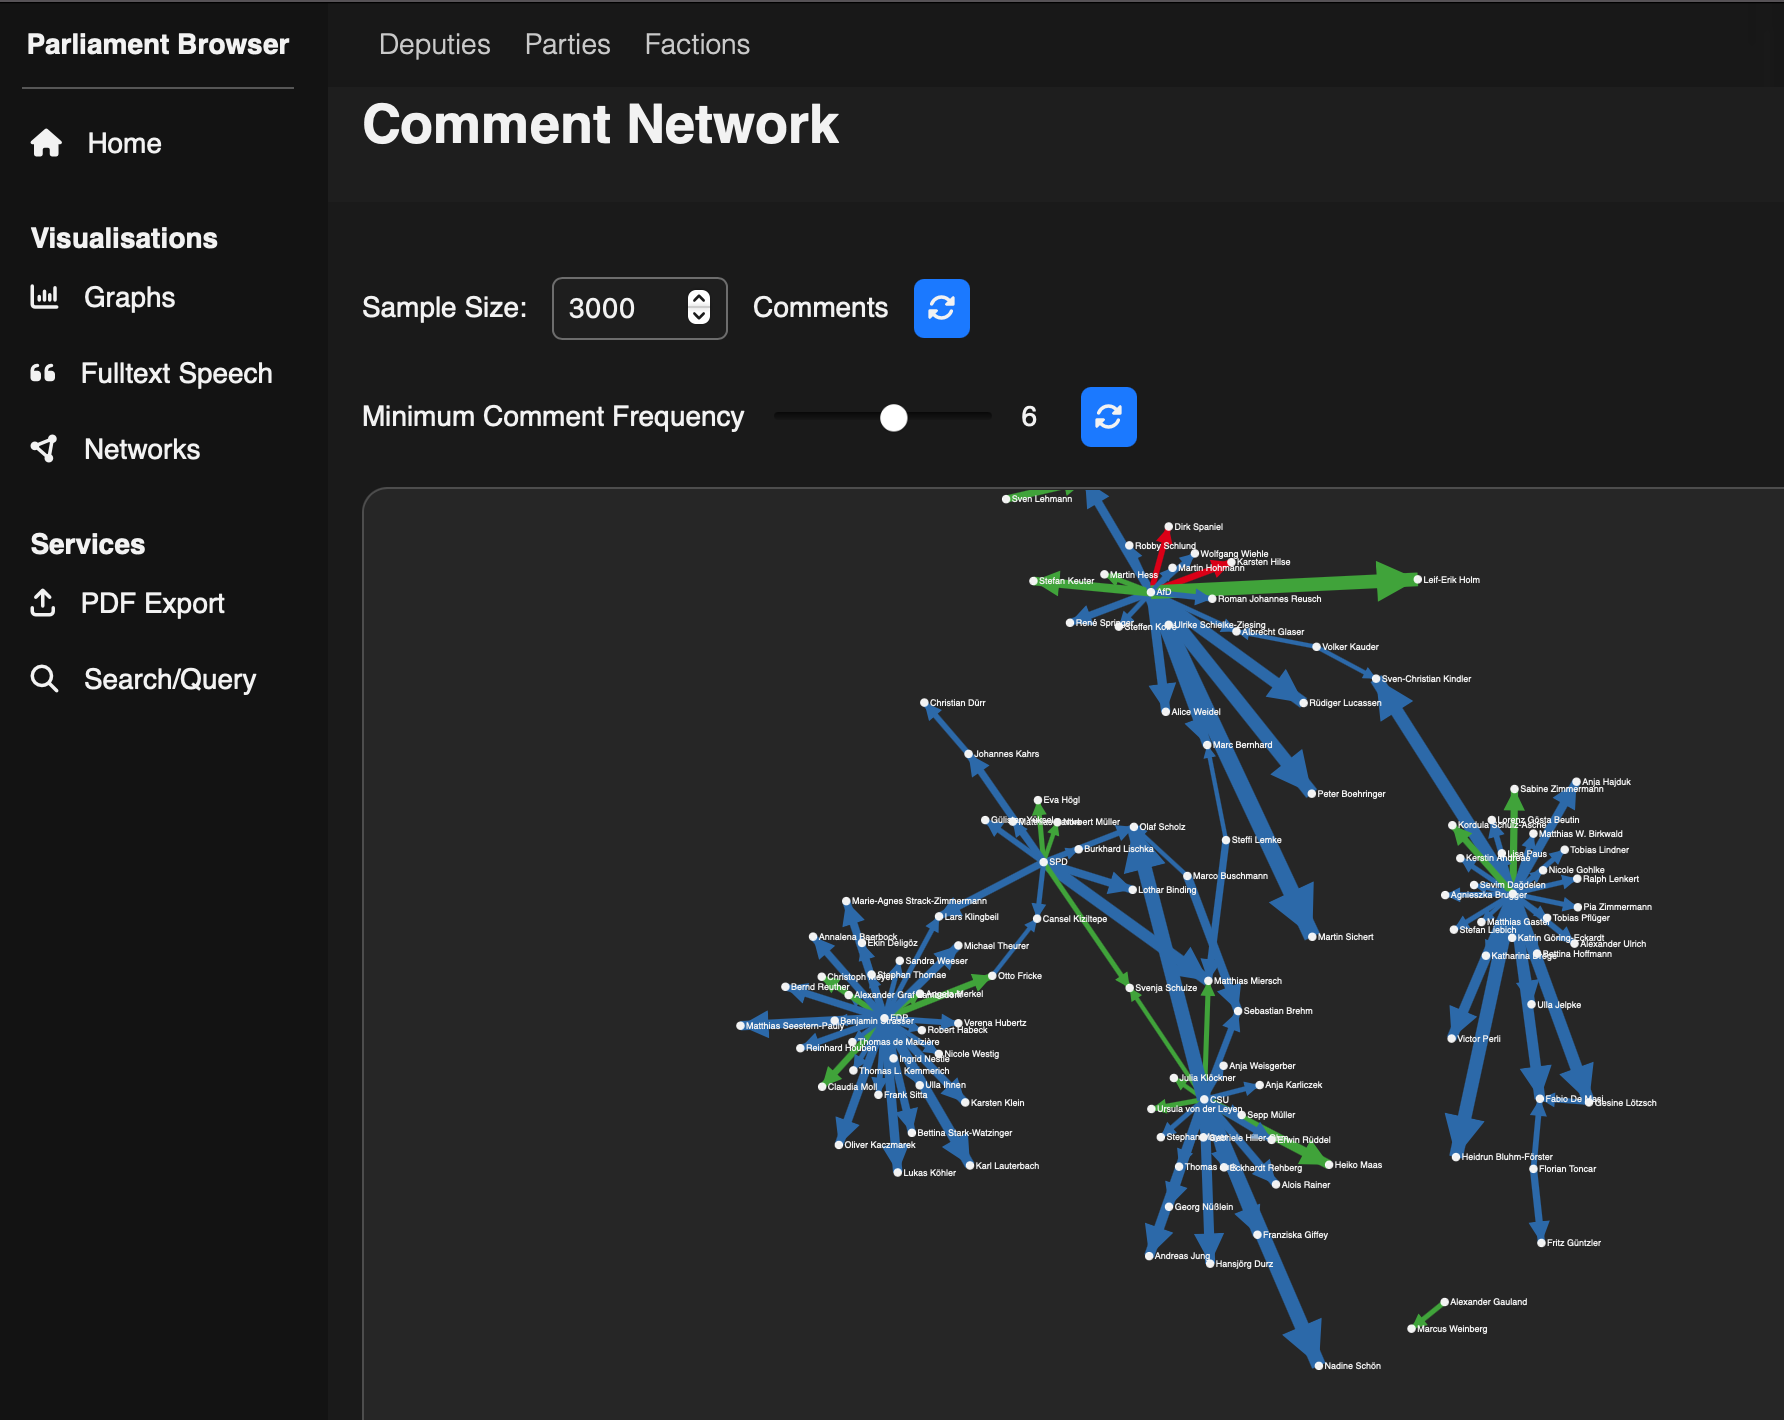
\includegraphics{commentNetwork_page1}}
  	 \end{center}
	\caption{Networks  $\quad\rightarrow\quad$  Route:  /commentNetwork}	
 \end{figure}
 

\noindent Im Mittelpunkt des Rede-Netzwerks, oder Speech Topic Network, steht nunmehr die Frage: Welche Redner:innen sprechen zu den gleichen Themen? Eine Art Topic-Analyse ist hier das Ziel der Illustration.\\
Route $\quad\rightarrow\quad$  /speechTopicNetwork\\\\
Die $Sample Size$ gibt wieder an, wie viele, diesmal Reden, in Betracht gezogen werden sollen. 
Der $Minimum Topic Score per Speech$ gibt an, wie relevant ein Thema in einer Rede gewesen sein muss, damit es berücksichtigt wird. Je höher der Wert desto relevanter.
Mit den blau hinterlegten Reload-Buttons können die Netzwerke mit den jeweils ausgewählten Parametern neu geladen werden.
Achtung! Ein niedrigen min. Topic Score und eine hohe Sample Size führen zu einer massiven Anzahl an Knoten und Kante im Netzwerk und wirken sich möglicherweise negativ auf die Performance der Website aus.\\\\
 
\begin{figure}[H]
	\begin{center}		
		\scalebox{0.3}{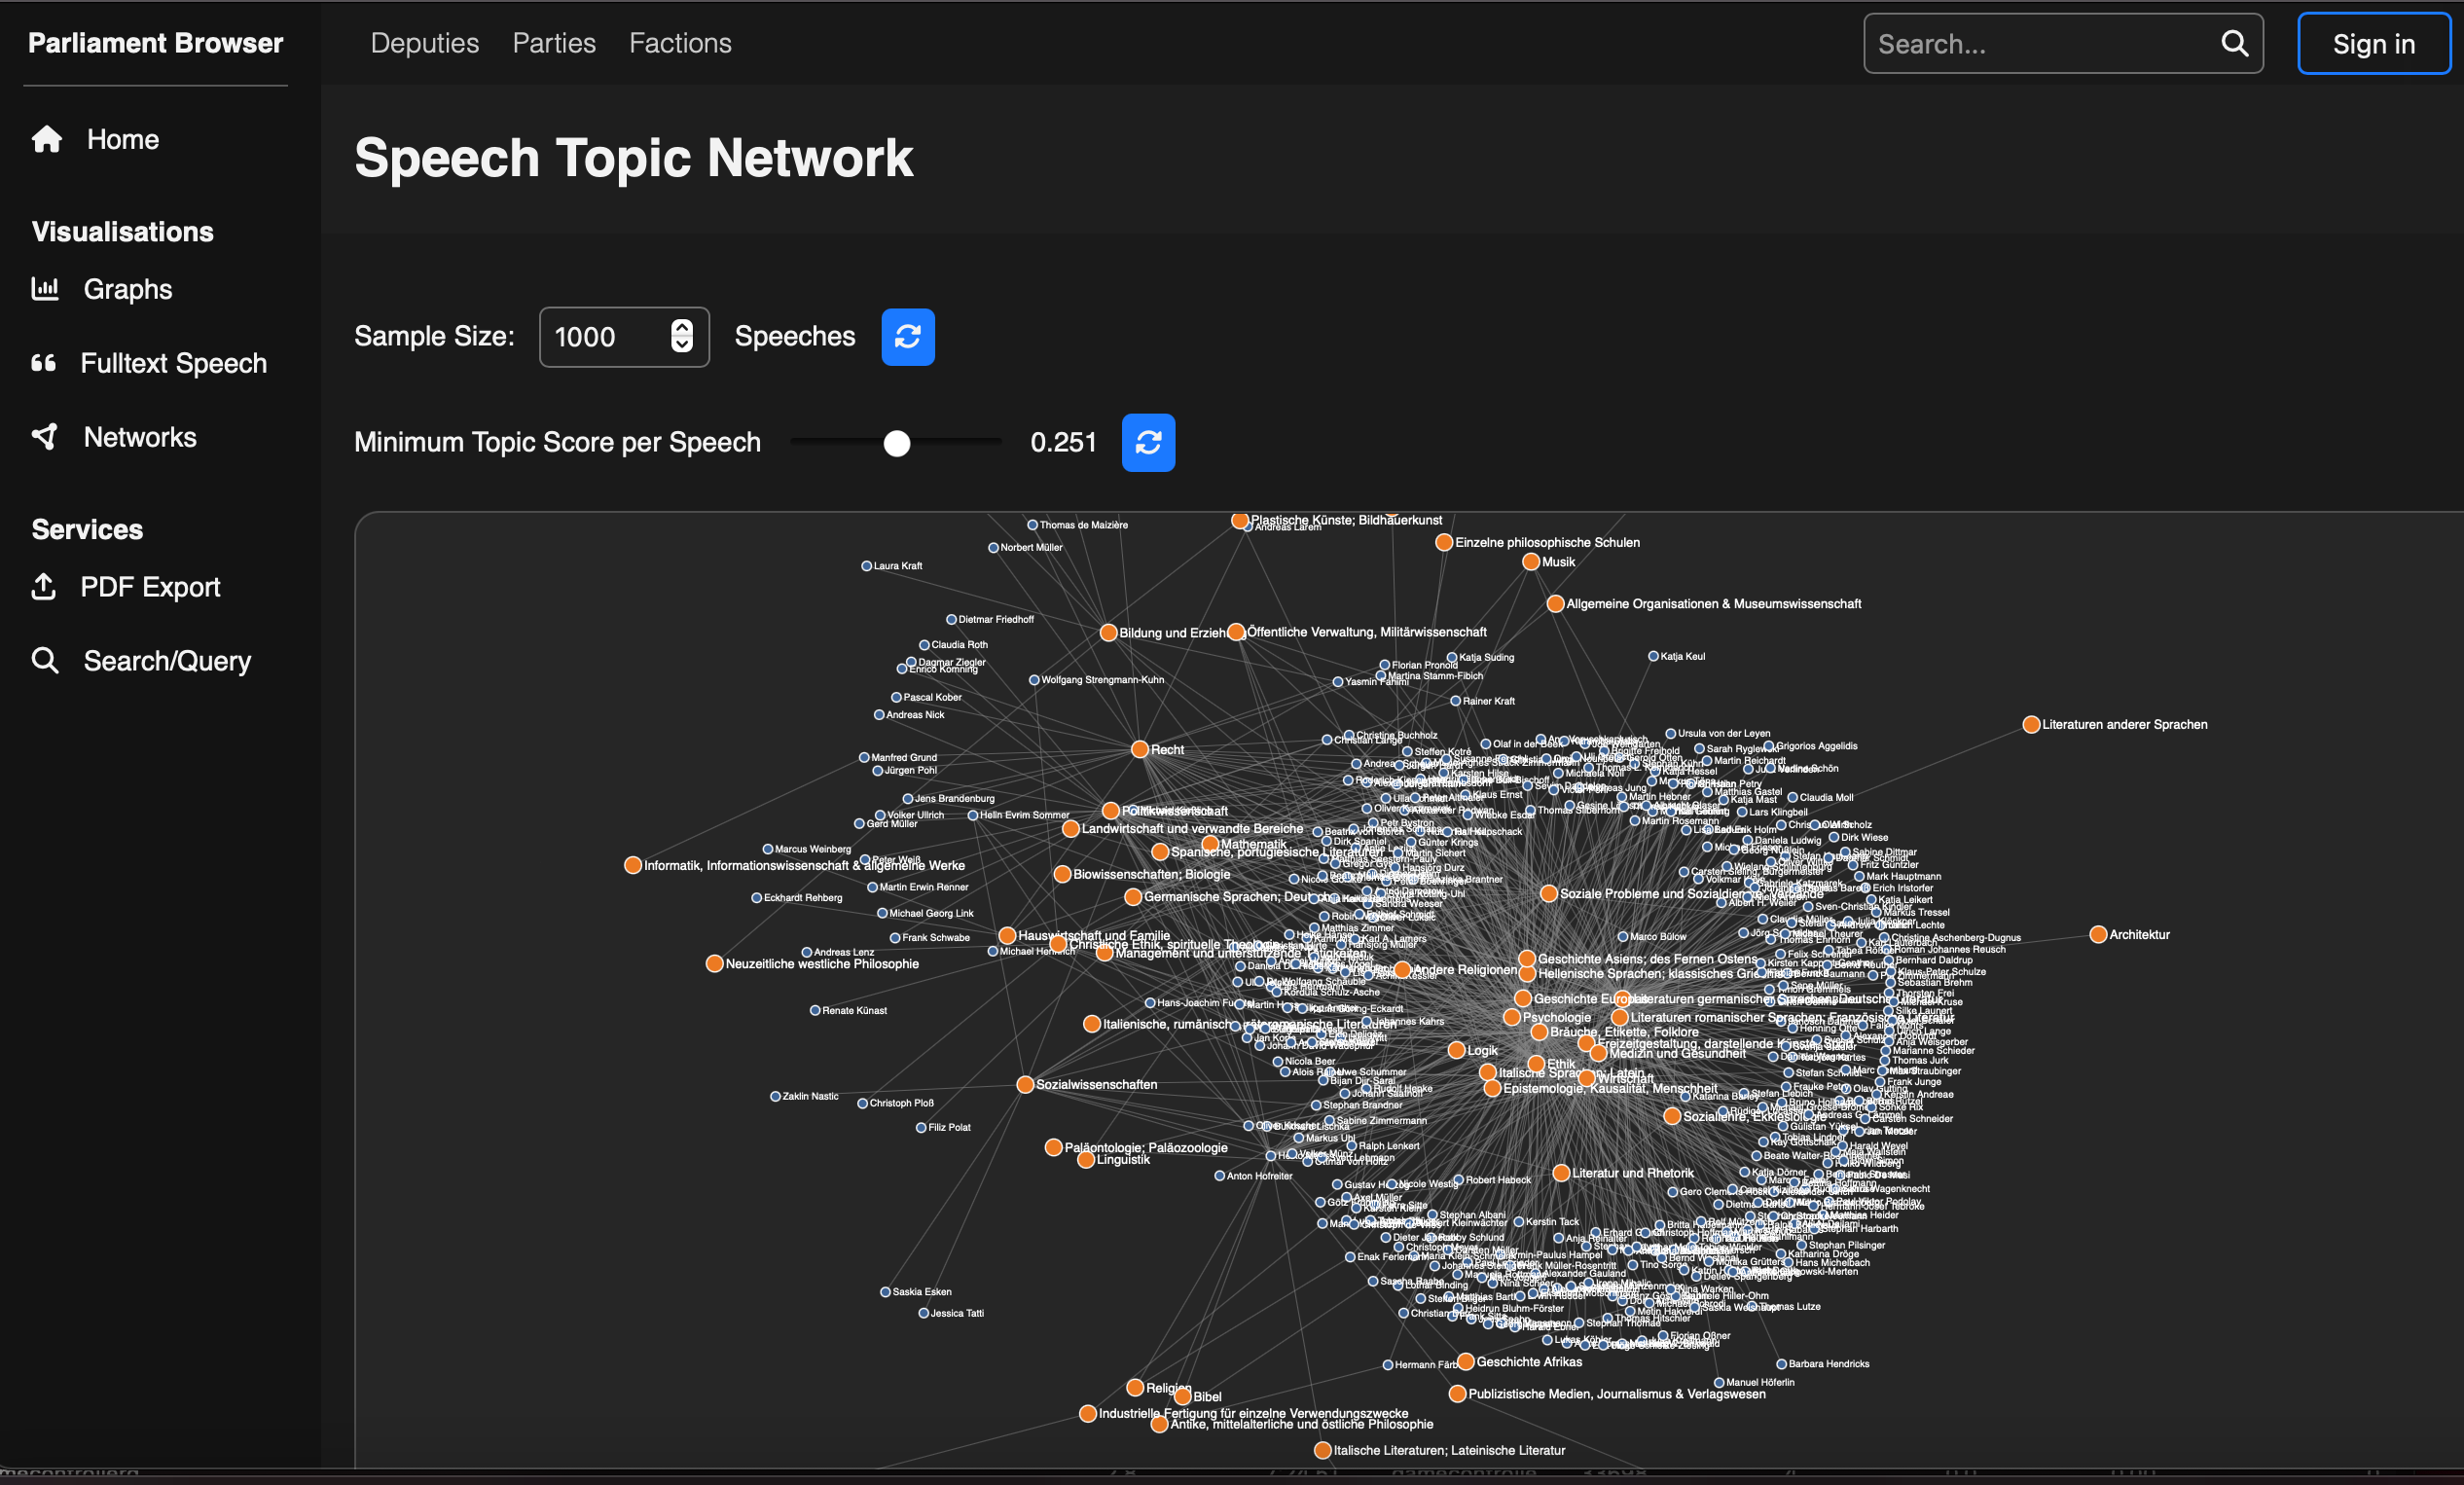
\includegraphics{speechTopicNetwork_page1}}
  	 \end{center}
	\caption{Networks  $\quad\rightarrow\quad$  Route:  /speechTopicNetwork}	
 \end{figure}

 
\noindent Als drittes Netzwerk stellen wir das Sentiment-Rede-Netzwerk vor, oder Speech Sentiment Network. 
Es illustriert den Zusammenhang zwischen Reden, den in diesen vorkommenden Kategorien und der darin übertragenden Stimmung wieder.
Die wählbaren Parameter verhalten sich anolog zu denen im Rede-Netzwerk.\\
Route $\quad\rightarrow\quad$  /speechSentimentNetwork\\\\ 
 
\begin{figure}[H]
	\begin{center}		
		\scalebox{0.35}{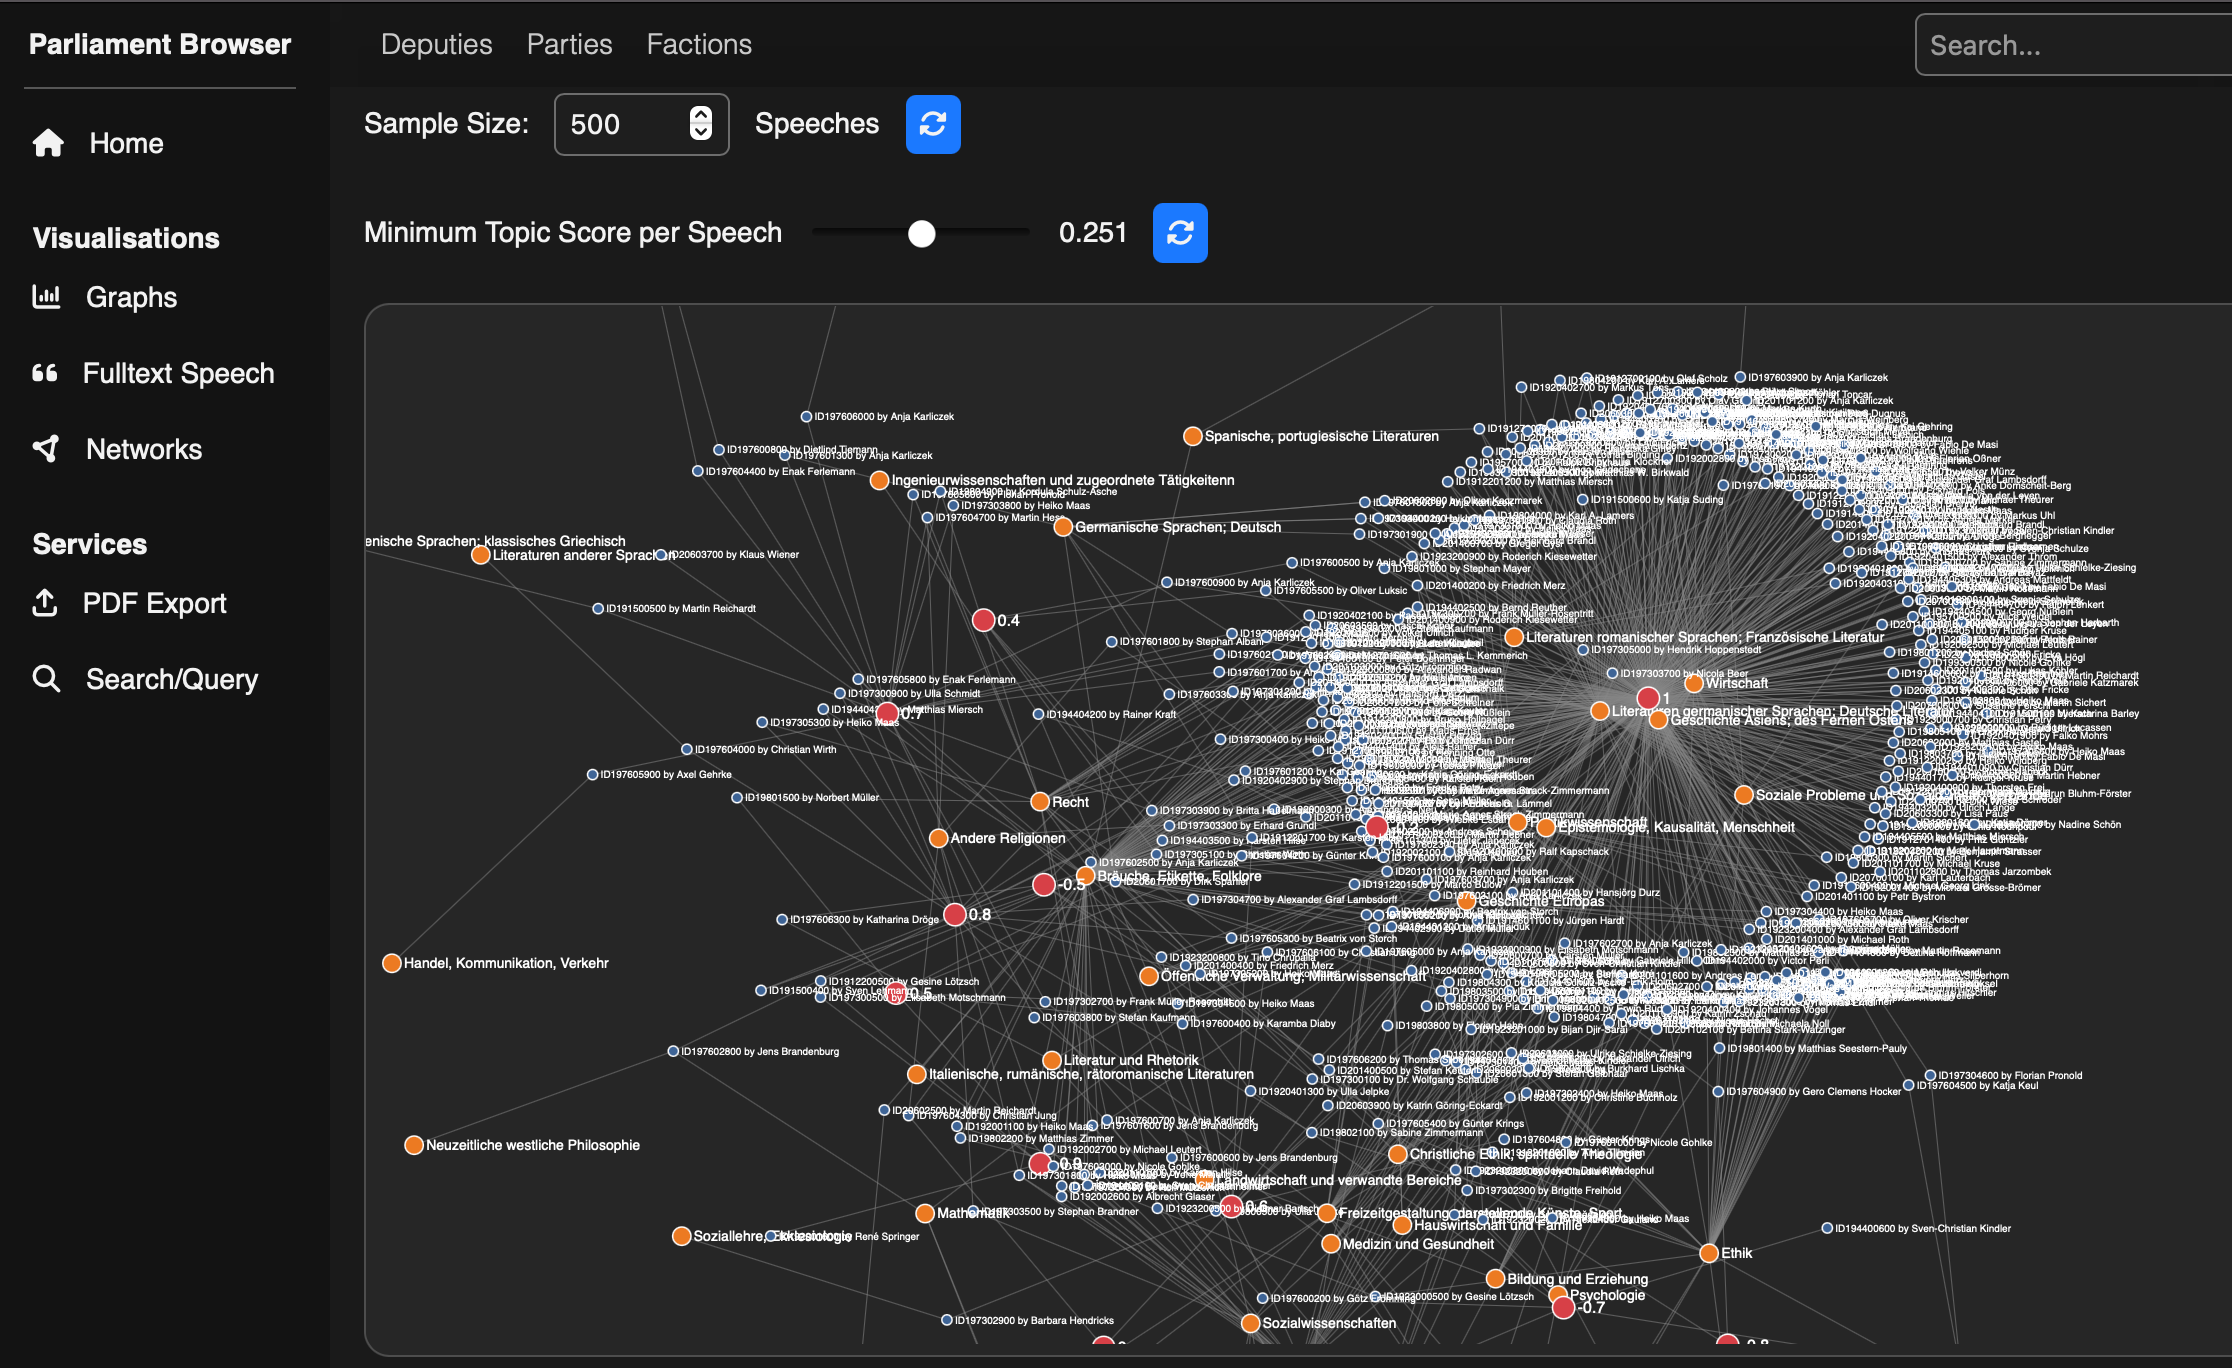
\includegraphics{speechSentimentNetwork_page1}}
  	 \end{center}
	\caption{Networks  $\quad\rightarrow\quad$  Route:  /speechSentimentNetwork}	
 \end{figure}


    
\chapter{Services}

       
\section{PDF Export  $\quad\rightarrow\quad$  Route:  /latexExport}

In diesem Menüpunkt geht es um den Export eines, intern in Latex generierten, Protokolls als PDF Dokument. Zunächst werden alle Protokolle in einer Liste am linken Bildausschnitt zur Verfügung gestellt. 
Bei Auswahl eines Protokolls kann über die Live-Preview des PDF-Dokuments im Inhaltsverzeichnis (Contents) ein Tagesordnungspunkt oder eine konkrete Rede ausgewählt und angeschaut werden. \\\\


\begin{figure}[H]
	\begin{center}		
		\scalebox{0.35}{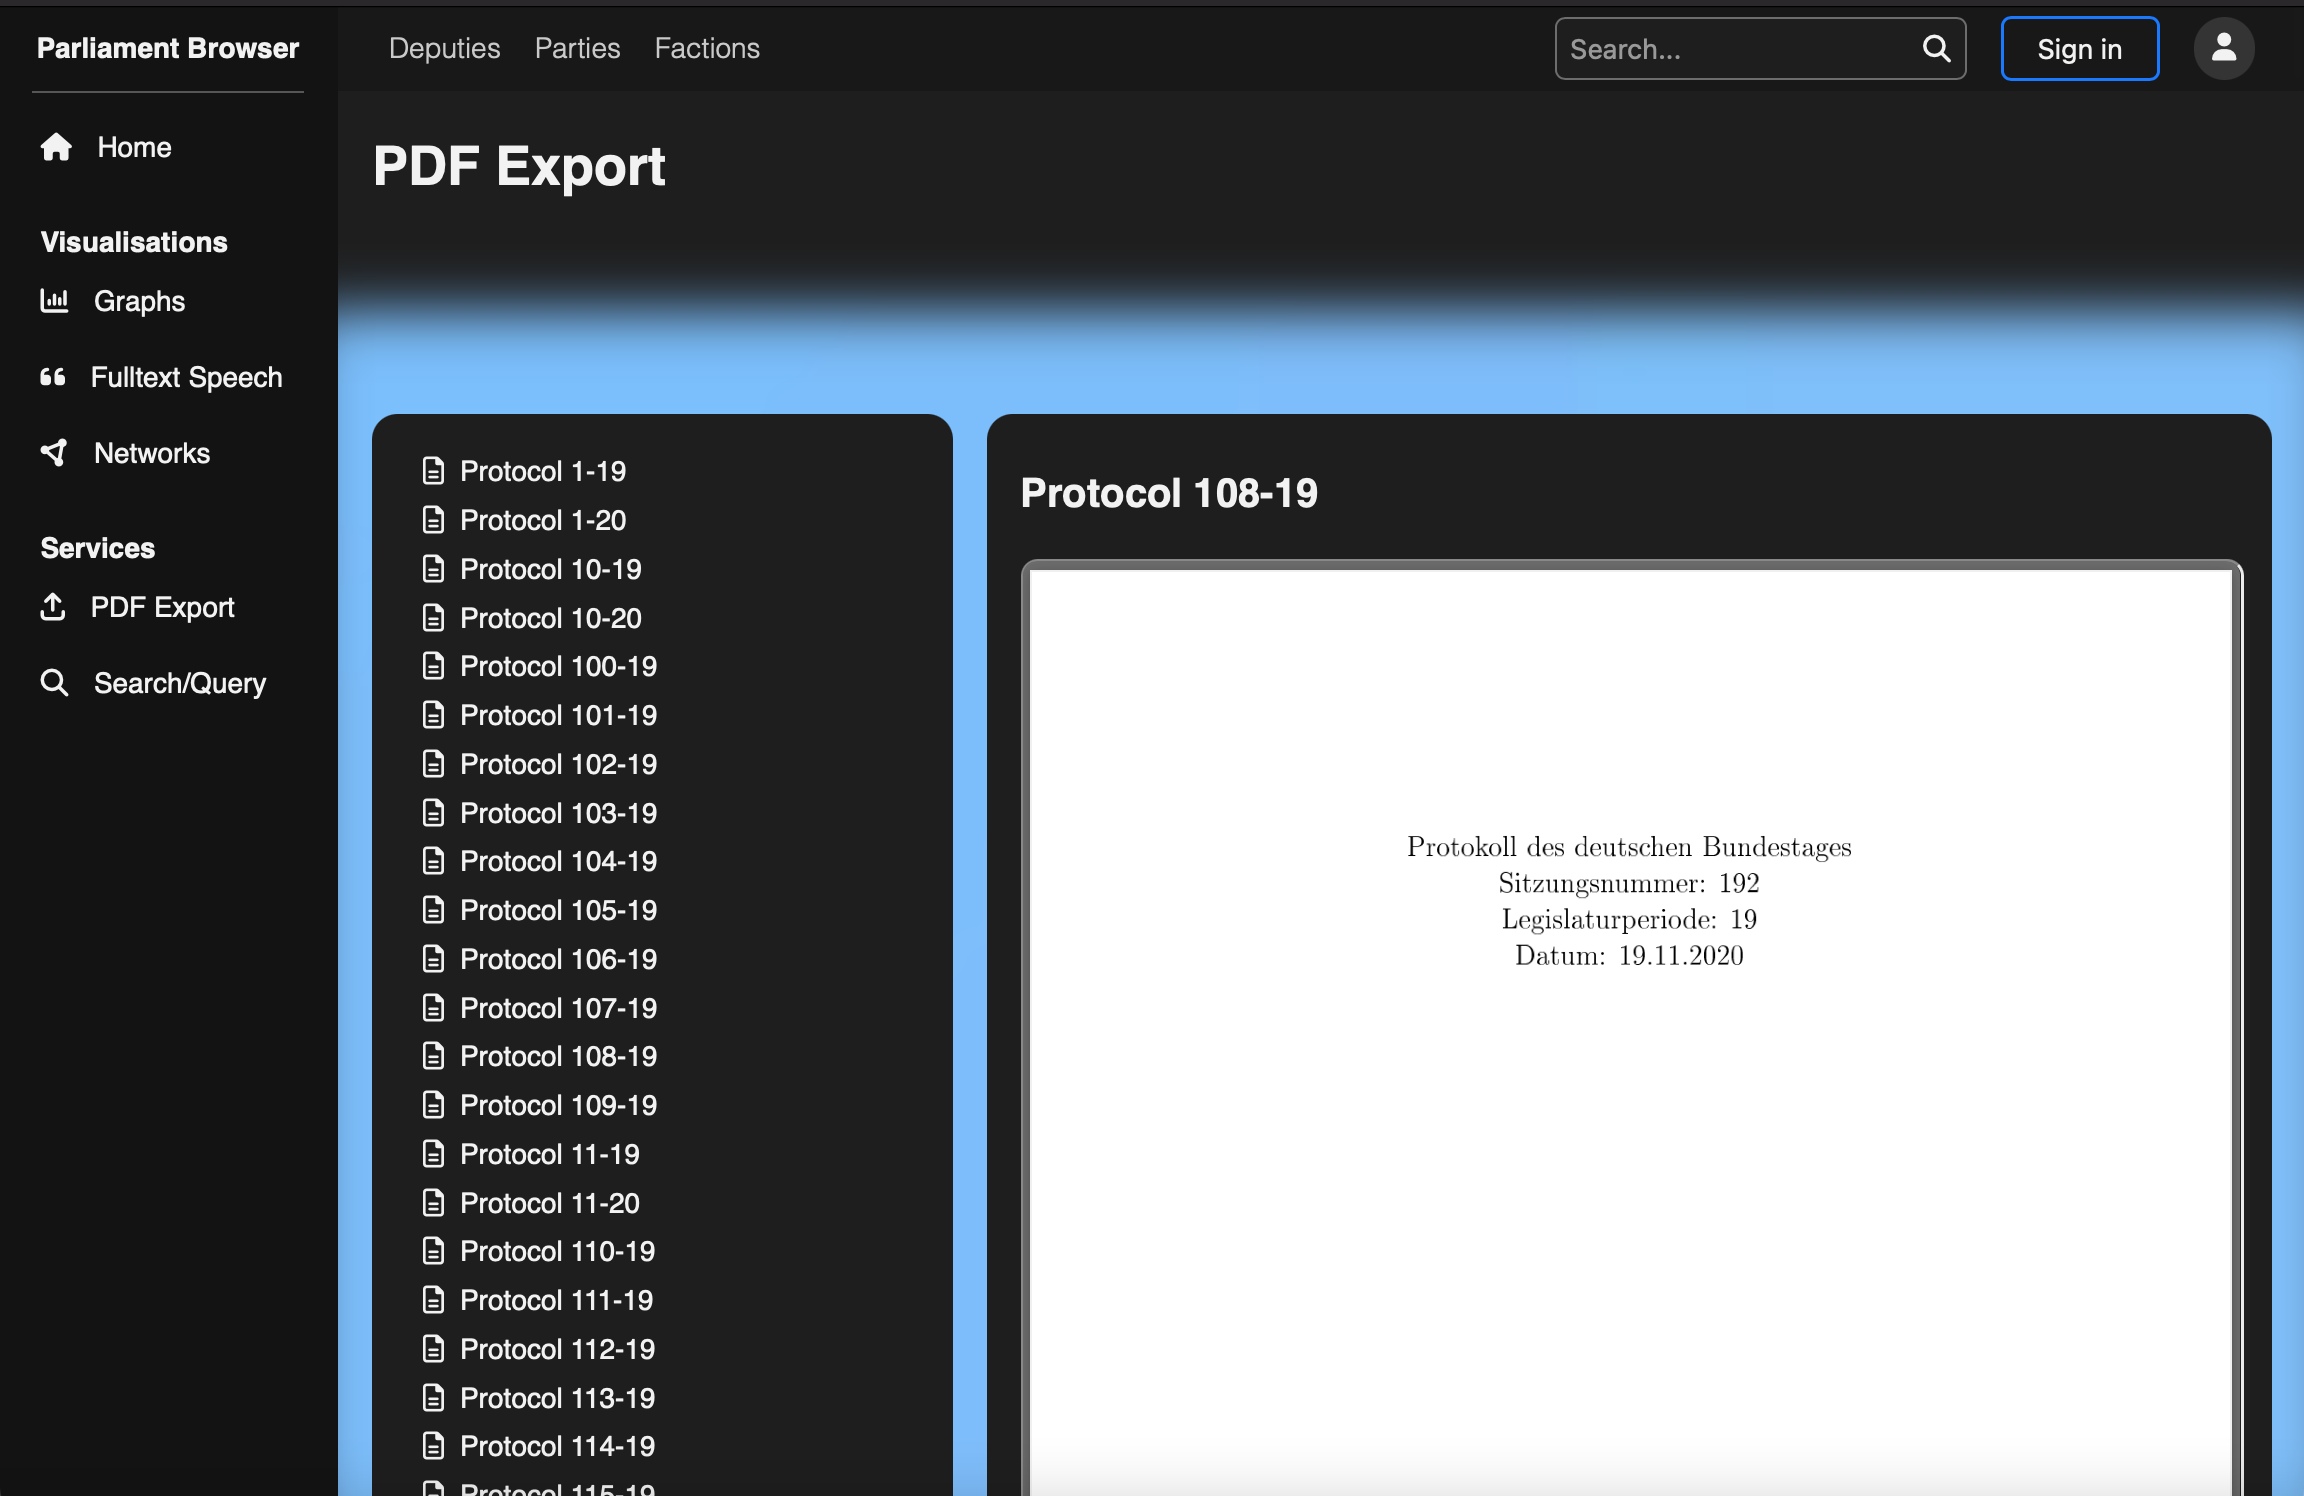
\includegraphics{latex_page1}}
  	 \end{center}
	\caption{PDF Export  $\quad\rightarrow\quad$  Route:  /latexExport}	
 \end{figure}

\noindent Zur Illustration einer Darstellung eines Tagesordnungspunktes oder einer Rede folgt ein Bild.

\begin{figure}[H]
	\begin{center}		
		\scalebox{0.35}{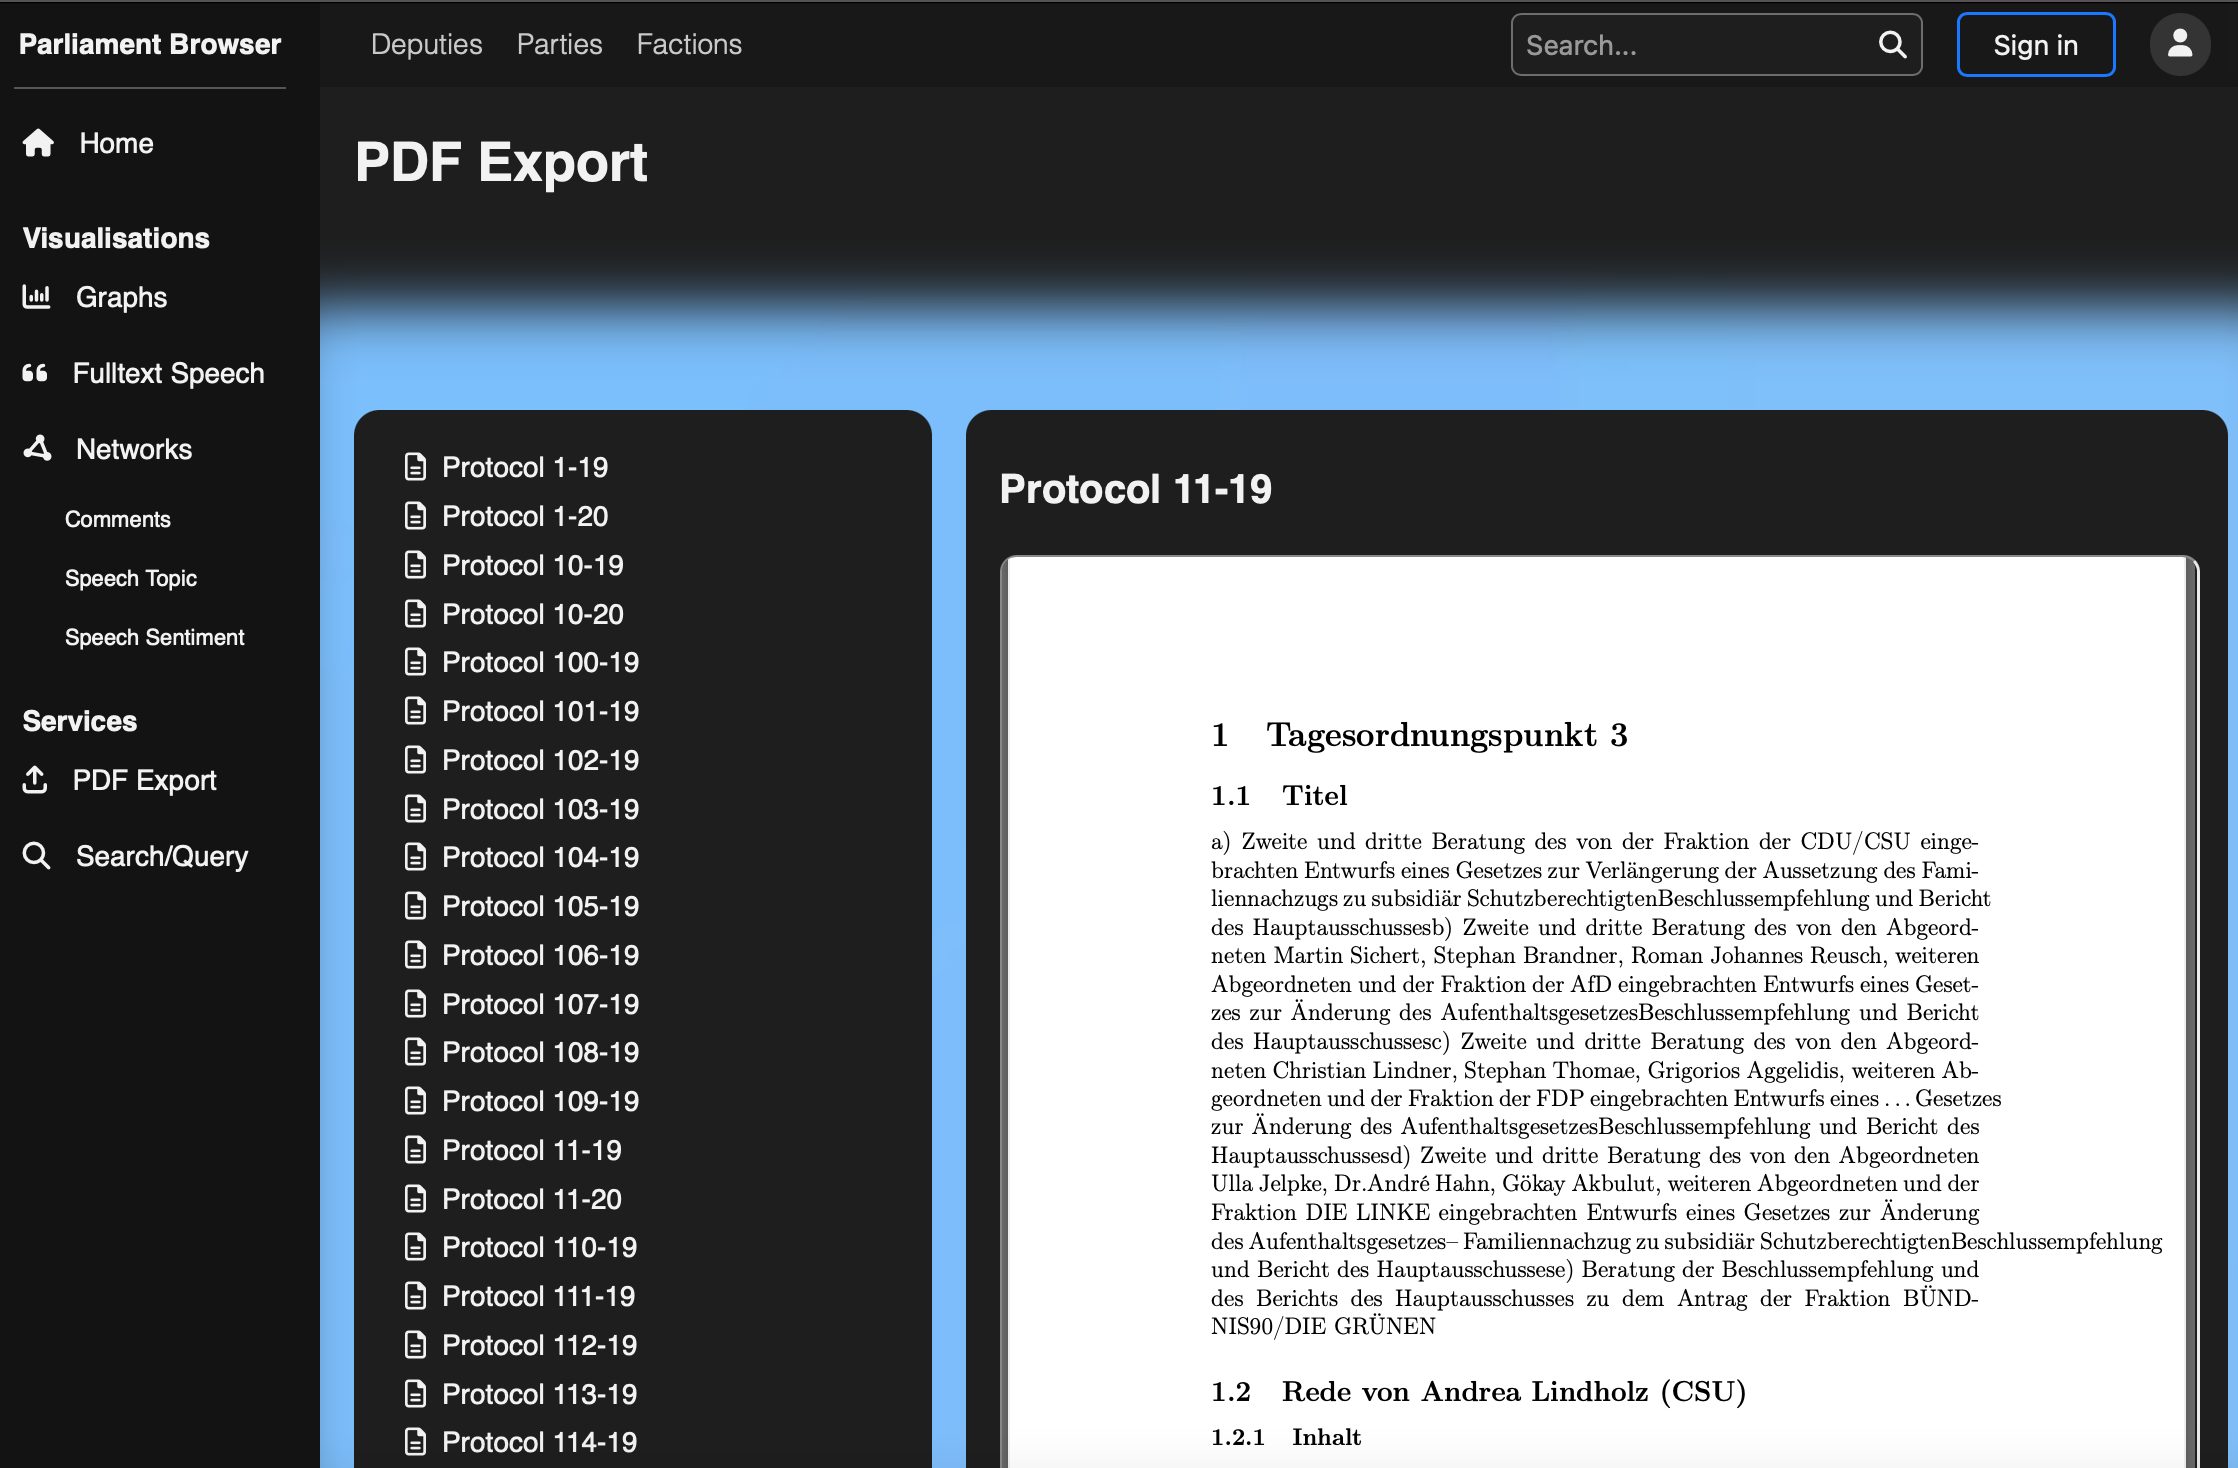
\includegraphics{latex_page2}}
  	 \end{center}
	\caption{PDF Export  $\quad\rightarrow\quad$  Route:  /latexExport}	
 \end{figure}


\section{Search/Query $\quad\rightarrow\quad$  Route:  /search}

Im Search/Query Bereich können Daten aus dem Parliament Browser angefragt werden. Die Wahlmöglichkeiten, nach denen Informationen angefragt werden können, sind vielfältig.
Alternativ zu dieser Seite kann auch die Allgemeine Suche in der oberen Navigationsleiste genutzt werden, falls nur nach einem bestimmten Begriff gesucht wird. \\
\begin{itemize}
\item Meta-Daten zu Abgeordneten lassen sich über die DeputyID, den Firstname oder den Lastname abrufen.
\item Informationen zu den Reden lassen sich über die Identifikations-Nummer, der SpeechID, zuordnen. 
Zusätzlich können Reden nach einem bestimmten Suchbegriff per Volltext-Suche gesucht werden.
Dieser ist im Feld $Term$ einzugeben.
\item Falls Interesse an Kommentaren zu Reden besteht, kann man sich diese auch anzeigen lassen. 
Dazu bitte die entsprechende Identifikations-Nummer, der CommentID, eingeben.
Aber auch hier besteht die Möglichkeit, Kommentare nach einem bestimmten Suchbegriff per Volltext-Suche zu suchen.
 \end{itemize}

  
\begin{figure}[H]
	  \begin{center}
		\scalebox{0.3}{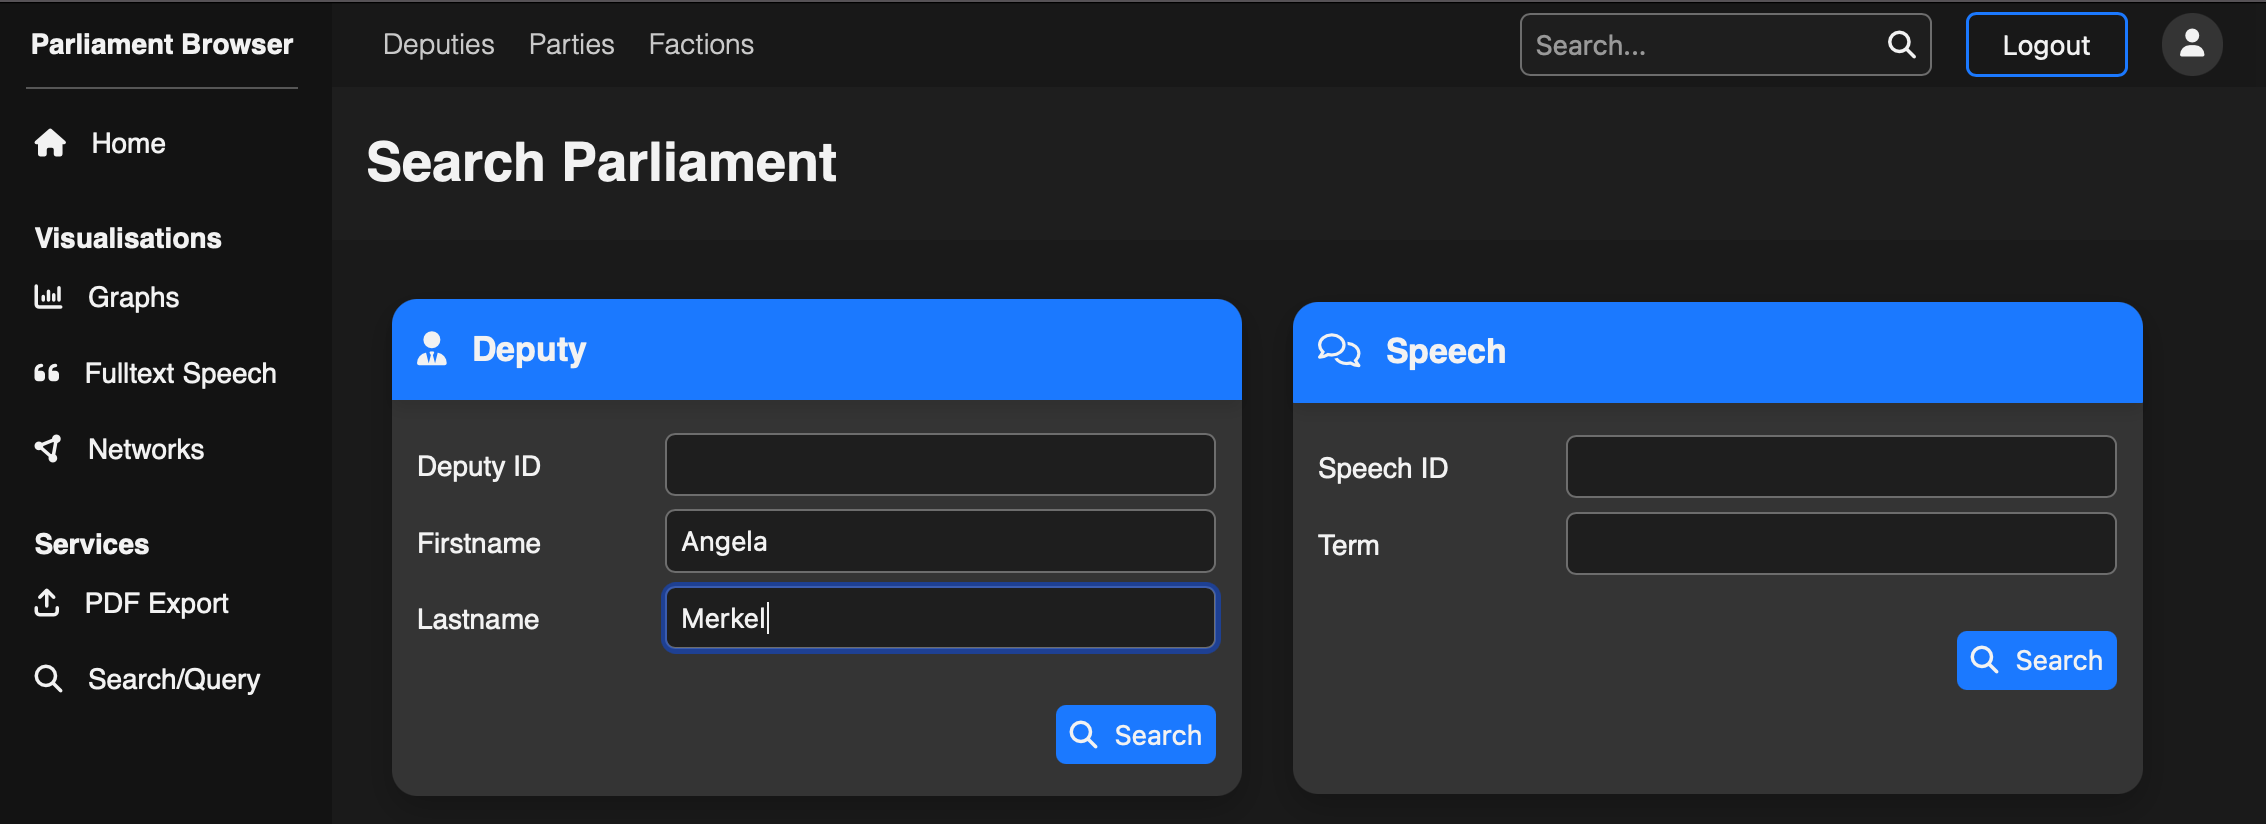
\includegraphics{search_page1}}
  	  \end{center}
	\caption{Search/Query  $\quad\rightarrow\quad$  Route:  /search} 
	\label{1}
\end{figure}
 \begin{figure}[H]
	  \begin{center}
		\scalebox{0.3}{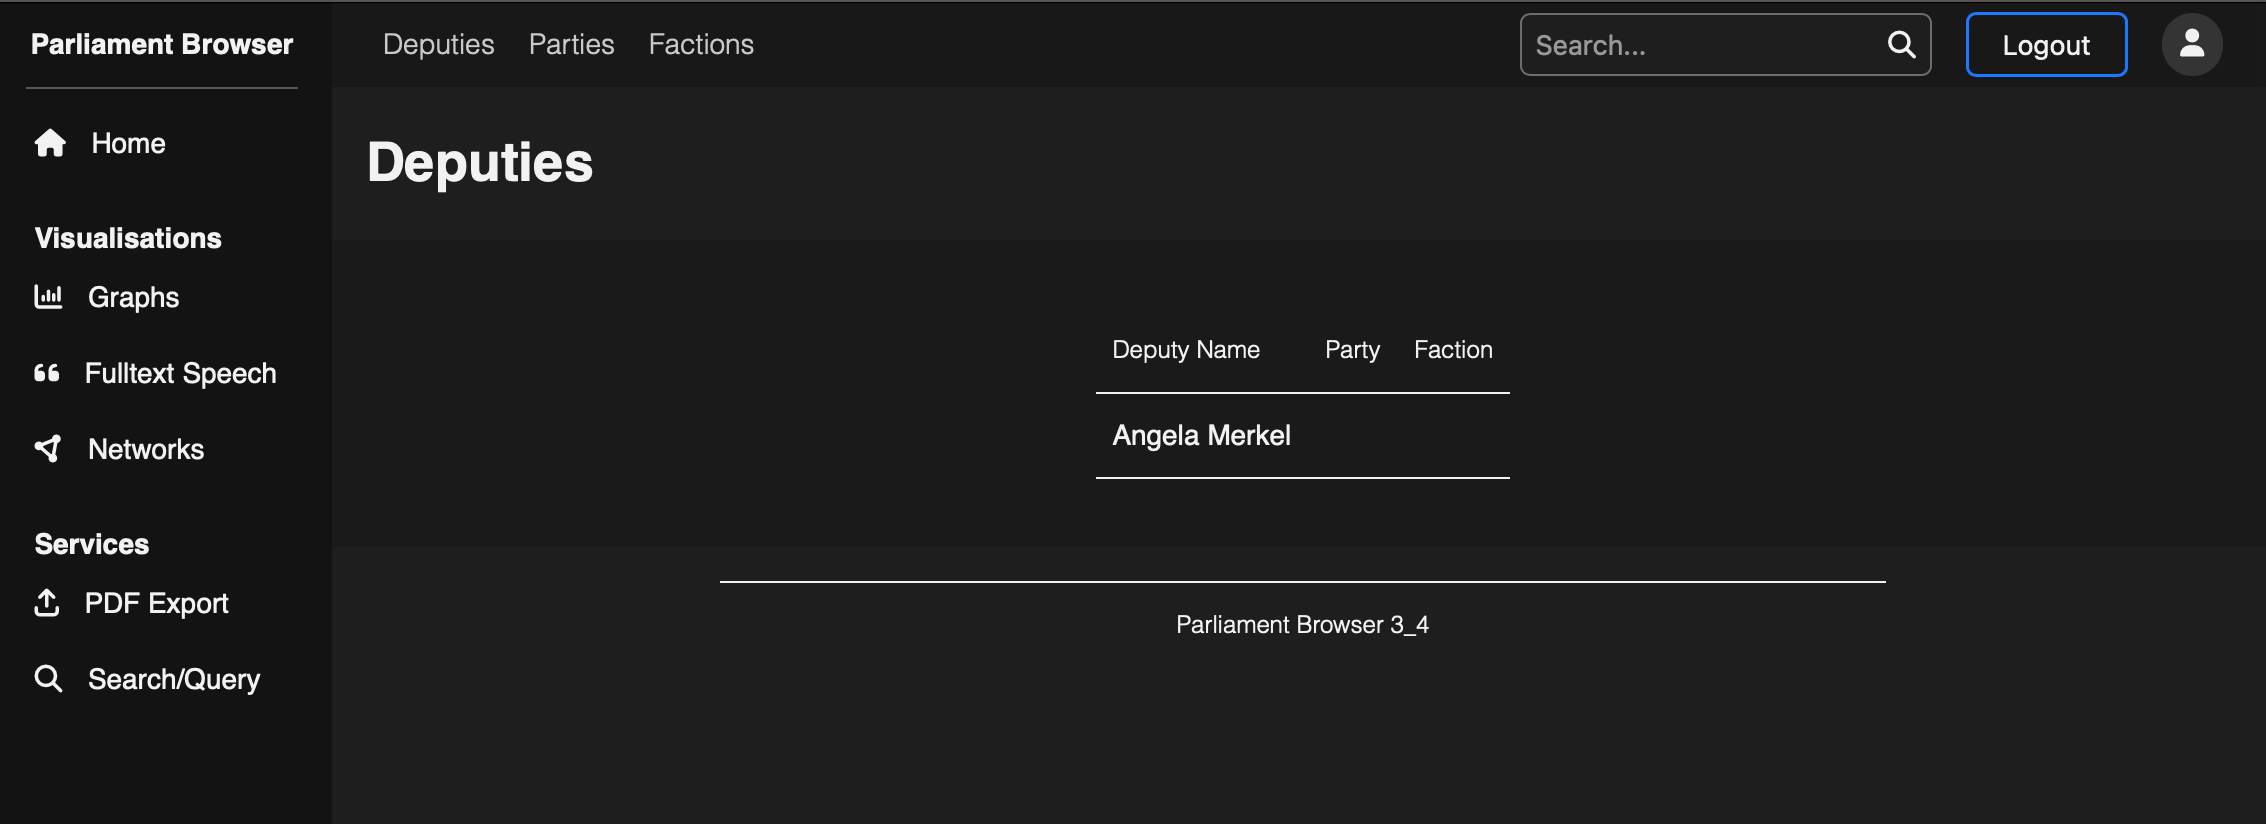
\includegraphics{search_page2}}
  	  \end{center}
	\caption{Search/Query  $\quad\rightarrow\quad$  Route:  /search}
	\label{1}
\end{figure}
\begin{figure}[H]
	  \begin{center}
		\scalebox{0.3}{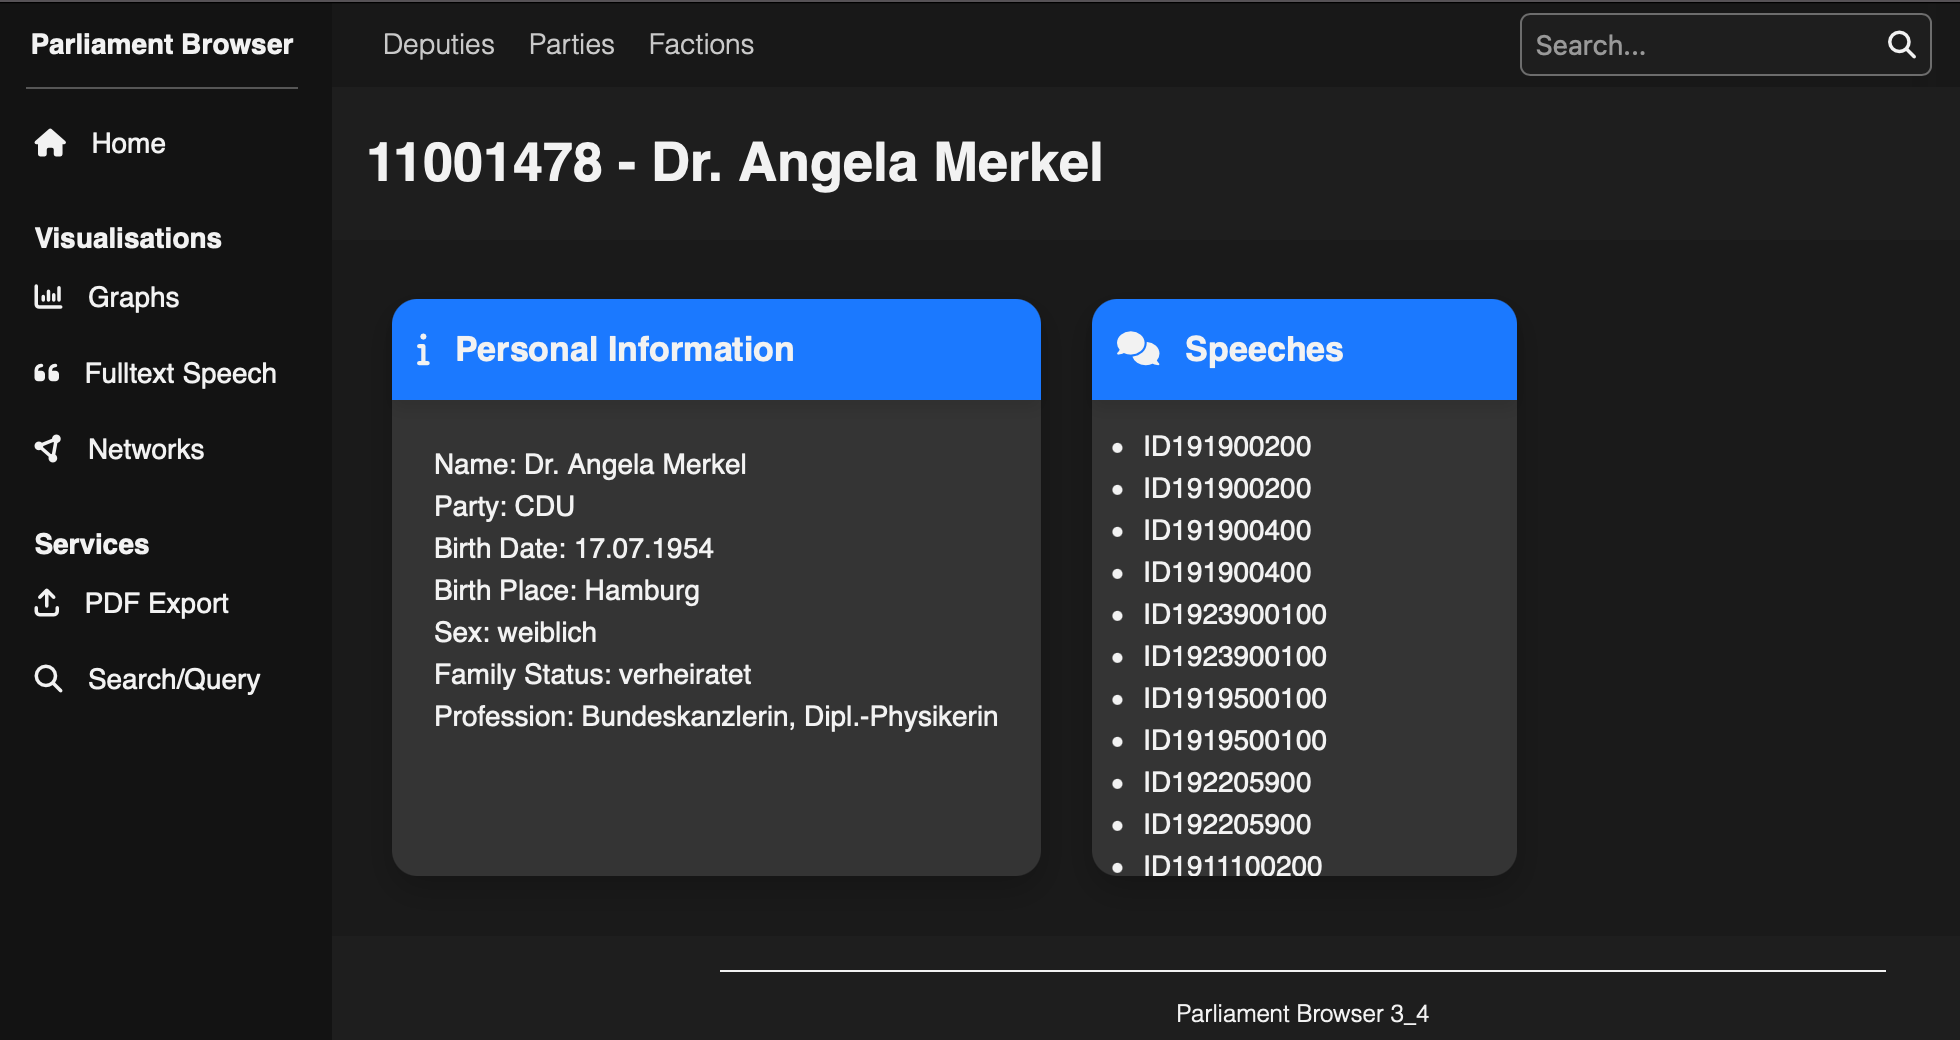
\includegraphics{search_page3}}
  	  \end{center}
	\caption{Search/Query  $\quad\rightarrow\quad$  Route:  /search}
	\label{1}
\end{figure} 
 
 
 
 
\chapter{System-Anforderungen}

\section{Java Spark Webserver}

\begin{itemize}
	\item Webserver: Java Version 1.8+
	\item Database: MongoDB Server Version 4.4.0+
	\item A Minimum of 4 GB RAM
	\item Broadband internet connection
	\item 200 MB of Free Disk Space 
\end{itemize}


\section{Browser Client}

\begin{itemize}
	\item Safari 15.4+, Chrome 98+, Edge 98+, Firefox 94+, Opera 84+
	\item Broadband internet connection
\end{itemize}


\end{document}